% !TEX root = main.tex
\documentclass[11pt,a4paper,spanish]{book}
\usepackage{Estilos/unir}

%---------------------------
% Rellenar con la información apropiada al Trabajo.
%---------------------------
\title{La Evolución de la Ciencia de Datos hacia la Computación Cuántica: Análisis de la Ventaja Cuántica en Casos Aplicados}
\titulacion{Máster en Computación Cuántica}
\author{Juan David Prada Malagón}
\date{\today}
\director{Ricardo Rafael Domínguez Reyes}
\nombreciudad{Barcelona, España}

\begin{document}

\maketitle

\frontmatter
\tableofcontents
\listoffigures
\listoftables
% !TEX root = ../main.tex
\chapter{Resumen}

La computación cuántica representa un paradigma emergente con potencial transformador para la ciencia de datos. Sin embargo, persiste una brecha significativa entre las promesas teóricas de los algoritmos cuánticos y su aplicabilidad práctica en entornos empresariales reales. Este trabajo propone un estudio comparativo riguroso entre algoritmos cuánticos —concretamente métodos de kernel cuántico y el algoritmo QAOA— y sus equivalentes clásicos —SVM, Random Forests y heurísticas de optimización— aplicados a problemas reales de clasificación supervisada y optimización combinatoria, utilizando datos procedentes de una empresa privada. Se evalúa el rendimiento mediante métricas de precisión, eficiencia computacional y escalabilidad. Adicionalmente, se diseña un prototipo conceptual de flujo de trabajo híbrido cuántico-clásico orientado a la integración práctica en pipelines productivos. Los resultados buscan aportar evidencia empírica sobre las condiciones reales de ventaja cuántica en ciencia de datos aplicada.

{\bf Palabras clave:} computación cuántica, ciencia de datos, ventaja cuántica, aprendizaje automático cuántico, QAOA
% !TEX root = ../main.tex
\chapter{Abstract}

Quantum computing represents an emerging paradigm with transformative potential for data science, yet a significant gap persists between the theoretical promises of quantum algorithms and their practical applicability on real-world data. This work presents a systematic empirical comparative study of quantum versus classical algorithms across eight use cases covering supervised classification (QSVM with quantum kernel), regression (QK-SVR), combinatorial optimisation (QAOA, VQE, SA-QUBO) and one-class anomaly detection (OCSVM-ZZ). Experiments are conducted on three dataset types per case when applicable: data with native quantum structure, practice data from SKG Tecnología (mobility incidents and travel times in Bogotá) and public-domain benchmarks.

Results show that quantum advantage is \emph{real but conditional}: QSVM achieves $+38.3$~pp over quantum-native data, while classical algorithms outperform in classification and regression on real-world data. In combinatorial optimisation, QAOA achieves a $-30.3\%$ cost reduction in resource assignment against greedy heuristics. Use Case~7 illustrates the \emph{hybrid quantum-classical paradigm} applied to the NP-hard minimum dominating set problem: the QAOA-COBYLA loop recovers the optimum with probability $\approx 73\%$. Use Case~8 (one-class anomalies, \emph{not} fraud) shows OCSVM-ZZ superior only when novelty is a ZZ phase on the same spatial support (AUC $0.864$ vs IsolationForest $0.553$); on moons/blobs and injected far outliers, IsolationForest wins.

Two original contributions are presented. The first is the \emph{quantumness score} $\mathcal{Q}(D)$, a composite metric based on kernel alignment ($\Delta A$), Frobenius distance ($d_F$) and differential spectral entropy ($\Delta H$), achieving a Spearman correlation of $\rho_S = 0.833$ ($p = 0.005$, $n = 9$) with empirical QSVM advantage. The second is the \emph{QCR Framework} (Quantum-Compatible Representation), a four-step protocol that automatically selects the optimal pre-mapping $T^*$: on Telco Churn it raises $\mathcal{Q}(D)$ from $-0.228$ to $+0.167$ and empirical advantage from $0$~pp to $+4.2$~pp via data re-uploading with \texttt{reps=3}. The practical conclusion is that quantum algorithms should be adopted as \emph{selective, complementary tools} within the enterprise technology stack — not as replacements for classical methods — being particularly promising for combinatorial optimisation with QUBO formulation. All experiments are conducted with Qiskit~2.3.0 on exact statevector simulation.

\vspace{0.5em}
\noindent\textbf{Keywords:} quantum computing, quantum machine learning, QSVM, quantum kernel, QAOA, VQE, combinatorial optimisation, anomaly detection, one-class SVM, variational algorithms, NISQ era, quantum advantage, quantumness score, QCR Framework.

\textbf{Keywords:} quantum computing, quantum advantage, hybrid quantum-classical algorithm, quantumness score, quantum kernel, QAOA, QSVM, OCSVM-ZZ, QCR Framework, minimum dominating set, NISQ


\mainmatter
% !TEX root = ../main.tex
\chapter{Introducción}

La computación cuántica representa uno de los paradigmas tecnológicos con mayor potencial transformador de las próximas décadas. Su capacidad para explotar fenómenos mecano-cuánticos como la superposición y el entrelazamiento abre la posibilidad de resolver problemas que resultan intratables para los computadores clásicos actuales \citep{preskill2018}. En paralelo, la ciencia de datos ha consolidado su posición como disciplina central en la toma de decisiones empresariales, apoyándose en algoritmos de aprendizaje automático, optimización combinatoria y análisis estadístico a gran escala \citep{jordan2015}. La convergencia de ambas disciplinas da lugar a un campo emergente con implicaciones profundas tanto para la investigación académica como para la práctica profesional.

Sin embargo, a pesar del creciente interés y del avance de los dispositivos cuánticos de escala intermedia ruidosa (NISQ, por sus siglas en inglés), persiste una brecha significativa entre las promesas teóricas de la computación cuántica y su aplicabilidad práctica en entornos reales de ciencia de datos \citep{preskill2018}. Los algoritmos variacionales cuánticos, como el Quantum Approximate Optimization Algorithm (QAOA) \citep{farhi2014} o los circuitos cuánticos variacionales (VQC) \citep{cerezo2021}, han emergido como las principales estrategias para aprovechar los dispositivos NISQ actuales, pero su ventaja frente a los métodos clásicos no está aún suficientemente demostrada en casos de uso empresariales reales.

Este trabajo aborda precisamente esa brecha, proponiendo un análisis comparativo riguroso y aplicado entre algoritmos cuánticos y clásicos en problemas representativos de la ciencia de datos.

\section{Motivación y justificación del tema}

La ciencia de datos, sustentada en técnicas de aprendizaje automático clásico, enfrenta limitaciones inherentes al paradigma de computación binaria cuando los problemas escalan en dimensionalidad o complejidad combinatoria \citep{biamonte2017}. Tareas como la clasificación de patrones en espacios de alta dimensión, la optimización de carteras de activos o la segmentación de clientes en grandes volúmenes de datos presentan costes computacionales que crecen de forma exponencial o polinómica con el tamaño del problema, lo que limita la capacidad de respuesta en entornos productivos con restricciones de tiempo.

La computación cuántica ofrece, en teoría, aceleraciones sustanciales para ciertos tipos de problemas. El algoritmo de Grover proporciona una aceleración cuadrática en búsquedas no estructuradas \citep{grover1996}, mientras que el algoritmo de Shor permite factorización en tiempo polinómico \citep{shor1994}. Más recientemente, los métodos de aprendizaje automático cuántico, en particular los basados en kernels cuánticos, han demostrado que los computadores cuánticos pueden acceder a espacios de características exponencialmente grandes, lo que podría suponer una ventaja real en tareas de clasificación \citep{haug2023}.

No obstante, el consenso científico actual es cauteloso. \cite{preskill2018} acuñó el término NISQ para describir la era actual de la computación cuántica, caracterizada por dispositivos con un número limitado de qubits y alta tasa de error, que aún no permiten implementar corrección de errores cuánticos a gran escala. En este contexto, resulta imprescindible evaluar de forma empírica y sistemática si los algoritmos cuánticos disponibles hoy en día pueden ofrecer ventajas medibles frente a sus equivalentes clásicos en problemas de ciencia de datos de relevancia empresarial.

La motivación de este trabajo surge precisamente de la necesidad de cubrir este vacío: no existen suficientes estudios comparativos que contrasten el rendimiento de algoritmos cuánticos con técnicas clásicas consolidadas sobre datos reales de negocio, evaluando no solo la precisión sino también la escalabilidad, el coste computacional y la viabilidad de integración en pipelines productivos.

\section{Planteamiento del problema}

El problema central que aborda este trabajo puede formularse de la siguiente manera: \textit{¿en qué condiciones, y para qué tipos de problemas de ciencia de datos, los algoritmos cuánticos disponibles en la era NISQ ofrecen una ventaja real y medible frente a los algoritmos clásicos?}

Para responder a esta pregunta, se plantea un estudio comparativo estructurado en torno a dos familias de problemas representativos: (1) problemas de \textbf{clasificación supervisada}, donde se comparará el rendimiento de clasificadores basados en kernels cuánticos frente a métodos clásicos como Support Vector Machines \citep{cortes1995} o Random Forests \citep{breiman2001}; y (2) problemas de \textbf{optimización combinatoria}, donde se evaluará el algoritmo QAOA \citep{farhi2014} frente a heurísticas clásicas como algoritmos genéticos o búsqueda local.

Los experimentos se realizarán sobre conjuntos de datos reales procedentes de una empresa privada, lo que garantiza la relevancia práctica de los resultados. Adicionalmente, se diseñará un prototipo conceptual de flujo de trabajo híbrido cuántico-clásico que ilustre cómo podrían integrarse estas tecnologías en arquitecturas de análisis de datos existentes \citep{cerezo2021}.

La aportación principal de este trabajo reside en proporcionar evidencia empírica sobre la viabilidad actual de la computación cuántica aplicada a la ciencia de datos, con una perspectiva orientada a la toma de decisiones en entornos empresariales reales, superando el enfoque puramente teórico o de laboratorio que predomina en la literatura existente \citep{fastovets2019}.

\section{Estructura del trabajo}

El presente trabajo se organiza en los siguientes capítulos:

El \textbf{Capítulo 2} presenta el contexto y la revisión de la técnica, describiendo los fundamentos de la computación cuántica relevantes para este trabajo, los principales algoritmos cuánticos aplicados a ciencia de datos y un análisis crítico de los trabajos previos más relevantes.

El \textbf{Capítulo 3} define los objetivos generales y específicos del trabajo, alineados con la brecha identificada en la revisión de la técnica.

El \textbf{Capítulo 4} integra la metodología de investigación adoptada y el diseño e implementación de las pruebas de concepto, describiendo las fases del estudio, los criterios de evaluación, el entorno tecnológico y la implementación detallada de los algoritmos cuánticos y clásicos, así como el diseño del flujo de trabajo híbrido prototipo.

El \textbf{Capítulo 5} recoge los resultados obtenidos, su análisis comparativo y la discusión sobre las implicaciones prácticas de los hallazgos.

El \textbf{Capítulo 6} expone las conclusiones del trabajo, sintetizando los hallazgos principales y su contribución al campo.

El \textbf{Capítulo 7} presenta las líneas de investigación futura que se derivan de los resultados y limitaciones identificadas a lo largo del estudio.
% !TEX root = ../main.tex
\chapter{Contexto y revisión de la técnica}

Este capítulo presenta los fundamentos conceptuales y el estado actual de la técnica en computación cuántica aplicada a la ciencia de datos. Se revisan los trabajos previos más relevantes, se identifican las limitaciones de los enfoques existentes y se sitúa la contribución de este trabajo en el contexto académico y profesional actual.

\section{Antecedentes históricos}

El origen formal de la computación cuántica como disciplina se remonta a los trabajos de \cite{feynman1982}, quien propuso el uso de sistemas cuánticos para simular la naturaleza de forma eficiente, argumentando que un computador clásico no podía simular un sistema cuántico sin un coste exponencial. Poco después, \cite{deutsch1985} formalizó el concepto de computador cuántico universal y demostró la existencia de problemas que un computador cuántico podría resolver de forma más eficiente que cualquier computador clásico.

El interés por la computación cuántica se intensificó con los algoritmos de \cite{shor1994} y \cite{grover1996}, que demostraron aceleraciones exponenciales y cuadráticas respectivamente frente a los mejores algoritmos clásicos conocidos para factorización de enteros y búsqueda no estructurada. Estos resultados establecieron la viabilidad teórica de la ventaja cuántica y sentaron las bases para el desarrollo de hardware cuántico experimental. Los fundamentos formales del modelo de computación cuántica, incluyendo los postulados de la mecánica cuántica, las puertas cuánticas y los circuitos cuánticos, se encuentran desarrollados en detalle en \cite{nielsen2010}.

En paralelo, el campo del aprendizaje automático experimentó un crecimiento extraordinario impulsado por el aumento de la capacidad computacional y la disponibilidad de grandes volúmenes de datos \citep{jordan2015}. La confluencia de ambas disciplinas dio lugar al campo del aprendizaje automático cuántico (\textit{Quantum Machine Learning}, QML), cuyo objetivo es explorar si las capacidades de procesamiento cuántico pueden ofrecer ventajas en tareas de aprendizaje estadístico \citep{biamonte2017}.

\section{Computación cuántica en la era NISQ}

El estado actual del hardware cuántico se enmarca en lo que \cite{preskill2018} denominó la era NISQ (\textit{Noisy Intermediate-Scale Quantum}), caracterizada por dispositivos con entre 50 y varios cientos de qubits físicos, afectados por errores de decoherencia y ruido cuántico, y sin capacidad para implementar corrección de errores cuánticos a gran escala. Esta realidad impone restricciones fundamentales sobre la profundidad de los circuitos ejecutables y la fiabilidad de los resultados obtenidos.

En respuesta a estas limitaciones, se han desarrollado los algoritmos variacionales cuánticos (\textit{Variational Quantum Algorithms}, VQA), que combinan un circuito cuántico parametrizado con un optimizador clásico en un bucle híbrido \citep{cerezo2021}. Entre los más destacados se encuentran el Quantum Approximate Optimization Algorithm (QAOA) \citep{farhi2014}, diseñado para problemas de optimización combinatoria, y el Variational Quantum Eigensolver (VQE) \citep{peruzzo2014}, orientado a la simulación de sistemas moleculares. Estos algoritmos son actualmente los candidatos más prometedores para demostrar ventaja cuántica práctica en hardware NISQ.

No obstante, la comunidad científica mantiene un debate activo sobre si los algoritmos NISQ pueden alcanzar ventaja cuántica genuina frente a los mejores algoritmos clásicos. \cite{cerezo2023} analizan en profundidad el fenómeno de los \textit{barren plateaus}, gradientes exponencialmente pequeños que dificultan el entrenamiento de los circuitos variacionales a medida que el número de qubits crece, comprometiendo la escalabilidad de estos enfoques.

\section{Aprendizaje automático cuántico}

El aprendizaje automático cuántico ha sido objeto de una revisión sistemática exhaustiva por parte de \cite{biamonte2017}, quienes identificaron cuatro categorías principales de algoritmos QML según la naturaleza del procesador (clásico o cuántico) y de los datos (clásicos o cuánticos). Para el contexto de este trabajo, el caso más relevante es el de datos clásicos procesados mediante algoritmos cuánticos (CC$\rightarrow$CQ en la nomenclatura de los autores).

Los métodos basados en kernels cuánticos (\textit{Quantum Kernel Methods}) han recibido especial atención. \cite{schuld2021} demostraron que los circuitos cuánticos pueden actuar como mapas de características (\textit{feature maps}) hacia espacios de Hilbert de alta dimensión, y que la estimación del kernel inducido puede ser computacionalmente difícil de simular clásicamente bajo ciertas condiciones. Sin embargo, \cite{huang2021} establecieron condiciones teóricas precisas bajo las cuales los kernels cuánticos pueden ofrecer una ventaja de aprendizaje sobre los kernels clásicos, concluyendo que dicha ventaja depende críticamente de la estructura geométrica de los datos de entrada.

En el contexto de la clasificación supervisada con datos reales, \cite{haug2023} propusieron el uso de medidas aleatorizadas para escalar los métodos de kernel cuántico a conjuntos de datos de gran tamaño, abordando uno de los principales cuellos de botella prácticos de estos métodos. Los resultados experimentales mostraron rendimientos competitivos frente a kernels clásicos en benchmarks estándar, aunque con una ventaja aún limitada.

\section{Optimización cuántica aplicada}

El QAOA, propuesto originalmente por \cite{farhi2014}, es un algoritmo híbrido cuántico-clásico que aproxima la solución de problemas de optimización combinatoria formulados como problemas de satisfacibilidad cuadráticas binarias (QUBO). Su aplicabilidad se extiende a problemas de relevancia empresarial como la optimización de rutas \citep{lucas2014}, la asignación de recursos, la segmentación de mercado y la optimización de carteras financieras.

\cite{zhou2020} estudiaron el rendimiento del QAOA en función de la profundidad del circuito ($p$) y demostraron que, para problemas de tamaño moderado, la calidad de la aproximación mejora monotónamente con $p$. No obstante, la ventaja cuántica del QAOA frente a los mejores algoritmos clásicos heurísticos sigue siendo una cuestión abierta para instancias de gran escala \citep{farhi2014}.

Desde una perspectiva aplicada, \cite{vikstaal2020} evaluaron la aplicabilidad del QAOA a problemas de optimización financiera reales, identificando los principales desafíos prácticos: la necesidad de un gran número de shots para estimar expectativas con precisión suficiente, la sensibilidad a los parámetros iniciales y la degradación del rendimiento en hardware ruidoso. Estos resultados subrayan la importancia de realizar evaluaciones experimentales sobre datos reales más allá de las pruebas de concepto teóricas.

\section{Análisis crítico de los trabajos previos}

La revisión de la literatura permite identificar un conjunto de limitaciones recurrentes en los estudios existentes que este trabajo pretende abordar:

\begin{itemize}
    \item \textbf{Uso predominante de datos sintéticos o académicos}: la mayoría de los estudios comparativos utilizan conjuntos de datos de benchmarks estándar (Iris, MNIST, MaxCut), que no reflejan la complejidad y el ruido inherentes a los datos empresariales reales \citep{biamonte2017, haug2023}.

    \item \textbf{Ausencia de comparación sistemática con métodos clásicos consolidados}: muchos trabajos evalúan el rendimiento cuántico de forma aislada, sin contrastar con técnicas clásicas de referencia como SVM, Random Forests o algoritmos genéticos en las mismas condiciones experimentales \citep{fastovets2019}.

    \item \textbf{Foco en la viabilidad teórica más que en la aplicabilidad práctica}: los análisis de ventaja cuántica suelen estar formulados en términos asintóticos o bajo supuestos ideales de hardware, sin considerar las restricciones reales de los dispositivos NISQ actuales \citep{cerezo2023}.

    \item \textbf{Escasa consideración de la integración en pipelines productivos}: los trabajos existentes raramente abordan la cuestión de cómo los módulos cuánticos podrían integrarse en arquitecturas de análisis de datos clásicas ya existentes en entornos empresariales \citep{cerezo2021}.
\end{itemize}

Este trabajo contribuye a superar estas limitaciones mediante un diseño experimental que combina datos reales de negocio, comparación directa con métodos clásicos de referencia y una evaluación orientada a la viabilidad de integración práctica.
% !TEX root = ../main.tex
\chapter{Objetivos}

La revisión de la técnica presentada en el capítulo anterior evidencia que, a pesar del avance teórico en computación cuántica aplicada a la ciencia de datos, persiste una brecha significativa entre los resultados obtenidos en condiciones ideales y los alcanzables en entornos productivos reales. Este trabajo se propone abordar dicha brecha mediante un análisis comparativo riguroso, orientado a la toma de decisiones en contextos empresariales. En este capítulo se definen los objetivos que guían la investigación.

\section{Objetivo general}

El objetivo general de este trabajo es evaluar de forma empírica y sistemática si los algoritmos cuánticos disponibles en la era NISQ ofrecen una ventaja real y medible frente a los algoritmos clásicos consolidados en problemas representativos de la ciencia de datos, utilizando datos procedentes de un entorno empresarial real, con el fin de determinar las condiciones bajo las cuales la computación cuántica puede aportar valor práctico en este dominio \citep{preskill2018, biamonte2017}.

\section{Objetivos específicos}

Para alcanzar el objetivo general, se establecen los siguientes objetivos específicos:

\begin{enumerate}
    \item \textbf{Identificar y caracterizar los conjuntos de datos empresariales} adecuados para el estudio comparativo, seleccionando problemas representativos de clasificación supervisada y optimización combinatoria con relevancia práctica demostrable.

    \item \textbf{Implementar y configurar los algoritmos cuánticos} seleccionados para el estudio, concretamente métodos de kernel cuántico y circuitos variacionales para clasificación \citep{schuld2021, huang2021}, así como el algoritmo QAOA para optimización \citep{farhi2014}, utilizando frameworks de simulación cuántica como Qiskit o PennyLane.

    \item \textbf{Implementar y configurar los algoritmos clásicos de referencia} correspondientes a cada problema, incluyendo Support Vector Machines (SVM), Random Forests y algoritmos heurísticos de optimización, siguiendo las mejores prácticas del campo \citep{jordan2015}.

    \item \textbf{Diseñar y ejecutar los experimentos comparativos} bajo condiciones controladas e idénticas para ambas familias de algoritmos, garantizando la reproducibilidad y la validez estadística de los resultados.

    \item \textbf{Evaluar el rendimiento comparativo} de los algoritmos cuánticos y clásicos mediante un conjunto de métricas cuantitativas que incluyan precisión, eficiencia computacional y escalabilidad, siguiendo criterios establecidos en la literatura \citep{cerezo2021, zhou2020}.

    \item \textbf{Analizar las condiciones de ventaja cuántica}, identificando los factores —como el tamaño del dataset, la dimensionalidad del problema o la profundidad del circuito— que determinan cuándo y en qué medida los algoritmos cuánticos superan a los clásicos \citep{huang2021, cerezo2023}.

    \item \textbf{Diseñar un prototipo conceptual de flujo de trabajo híbrido} cuántico-clásico que ilustre cómo los módulos cuánticos podrían integrarse en arquitecturas de análisis de datos existentes en entornos empresariales \citep{cerezo2021}.
\end{enumerate}

% !TEX root = ../main.tex
\chapter{Metodología de diseño e implementación de las pruebas de concepto}
\label{cap:metodologia}

Este capítulo integra la metodología adoptada y la descripción detallada del diseño, implementación y procedimiento experimental de las pruebas de concepto (PoC) desarrolladas para comparar algoritmos cuánticos y clásicos en tres familias de problemas: clasificación supervisada, regresión y optimización combinatoria. Para cada caso de uso se evalúan tres tipos de conjuntos de datos: (i) un dataset diseñado con estructura cuántica explícita (\textit{cuántico-nativo}), (ii) un dataset real de SKG Tecnología, y (iii) un dataset de referencia de dominio público. Esta triple perspectiva permite distinguir los escenarios donde la computación cuántica ofrece ventaja teórica genuina de aquellos donde los algoritmos clásicos siguen siendo superiores en la práctica.

% =====================================================================
\section{Metodología general}
% =====================================================================

La metodología adoptada en este trabajo combina un enfoque experimental cuantitativo con un análisis crítico de los resultados desde la perspectiva de la aplicabilidad empresarial. Se articula en las siguientes fases:

\subsection{Fase 1: Selección y preparación de datos}

Se utilizaron conjuntos de datos reales procedentes de una empresa privada, relacionados con problemas de clasificación de clientes y optimización de asignación de recursos. Los datos fueron anonimizados y tratados conforme a las buenas prácticas de protección de datos. En caso necesario, se complementó el análisis con datos sintéticos generados a partir de distribuciones similares para garantizar la robustez de los resultados y preservar la confidencialidad. Los datasets fueron preprocesados siguiendo técnicas estándar de ciencia de datos: normalización, tratamiento de valores ausentes y reducción de dimensionalidad cuando fue necesario \citep{jordan2015}.

\subsection{Fase 2: Implementación de algoritmos}

Los algoritmos cuánticos se implementaron en simulación clásica mediante el framework \textit{Qiskit} (IBM), que permite simular circuitos cuánticos de hasta decenas de qubits en hardware clásico con ruido controlado. Para los problemas de clasificación se implementaron clasificadores basados en kernels cuánticos \citep{schuld2021} y circuitos variacionales (VQC) \citep{cerezo2021}. Para los problemas de optimización se implementó el QAOA con diferentes valores de profundidad $p$ \citep{farhi2014, zhou2020}. Los algoritmos clásicos de referencia se implementaron mediante las bibliotecas estándar de \textit{scikit-learn} y \textit{scipy}.

\subsection{Fase 3: Diseño experimental y evaluación}

Los experimentos se diseñaron siguiendo un protocolo de validación cruzada estratificada para los problemas de clasificación, y un esquema de múltiples ejecuciones con semillas aleatorias controladas para los problemas de optimización. Las métricas de evaluación principales fueron:

\begin{itemize}
    \item \textbf{Clasificación}: exactitud (\textit{accuracy}), precisión, exhaustividad (\textit{recall}) y puntuación F1, junto con el área bajo la curva ROC (AUC-ROC).
    \item \textbf{Optimización}: valor de la función objetivo alcanzada, razón de aproximación respecto al óptimo clásico conocido y tiempo de convergencia.
    \item \textbf{Eficiencia computacional}: tiempo de ejecución total, número de qubits requeridos, profundidad del circuito y número de evaluaciones de la función objetivo.
    \item \textbf{Escalabilidad}: evolución del rendimiento en función del tamaño del problema, evaluada mediante experimentos con instancias de tamaño creciente.
\end{itemize}

\subsection{Fase 4: Diseño del prototipo híbrido}

A partir de los resultados obtenidos, se diseñó un flujo de trabajo conceptual que integra el módulo cuántico de mejor rendimiento dentro de una arquitectura de análisis de datos clásica. Este prototipo ilustra los puntos de integración entre componentes cuánticos y clásicos, los requisitos de interfaz y las condiciones de activación del módulo cuántico, proporcionando una visión práctica orientada a la adopción tecnológica futura \citep{cerezo2021}.

Para cada caso de uso se evalúan tres tipos de conjuntos de datos: (i) un dataset diseñado con estructura cuántica explícita (\textit{cuántico-nativo}), (ii) un dataset real de SKG Tecnología, y (iii) un dataset de referencia de dominio público. Esta triple perspectiva permite distinguir los escenarios donde la computación cuántica ofrece ventaja teórica genuina de aquellos donde los algoritmos clásicos siguen siendo superiores en la práctica.

% =====================================================================
\section{Entorno tecnológico y arquitectura experimental}
% =====================================================================

Todos los experimentos se ejecutaron en simulación clásica exacta mediante \textit{Qiskit 2.3.0} \citep{Qiskit}, empleando el \texttt{StatevectorSimulator} que evalúa circuitos cuánticos de manera determinista y sin ruido, aislando el efecto del algoritmo cuántico de las imperfecciones del hardware real. Los modelos clásicos se implementaron con \textit{scikit-learn 1.8.0} y \textit{XGBoost 3.2.0}. El entorno fue Python 3.14 sobre una máquina Apple M-series con 16~GB de RAM. Todos los experimentos están disponibles en notebooks Jupyter reproducibles.

La elección del simulador de vector de estados garantiza exactitud matemática, pero no captura el ruido cuántico inherente al hardware NISQ real. Esto constituye simultáneamente una fortaleza metodológica ---se evalúa el potencial teórico del algoritmo--- y una limitación práctica: los resultados en hardware real serán necesariamente inferiores debido a la decoherencia y los errores de puerta. Esta distinción se aborda explícitamente en cada caso de uso.

% =====================================================================
\section{Caso de uso 1: Clasificación supervisada con kernel cuántico}
% =====================================================================

\subsection{Descripción del problema}

El primer caso de uso aborda la clasificación binaria supervisada, comparando el QSVM (Quantum Support Vector Machine con kernel cuántico) frente a cuatro clasificadores clásicos de referencia: Gradient Boosting, Random Forest, SVM-RBF y Regresión Logística. La hipótesis central, fundamentada en \cite{liu2021}, establece que cuando las etiquetas de clase se derivan de una función cuántica, el kernel cuántico aprende el problema con precisión cuasi-perfecta mientras que los clasificadores clásicos están limitados por el denominado \textit{quantum hardness} del problema.

% ---
\subsection{Dataset 1: Cuántico-nativo (Liu 2021)}

\paragraph{Descripción y justificación.}
Siguiendo el protocolo de \cite{liu2021}, se generó un dataset sintético donde las etiquetas binarias se definen mediante la expectación de un observable cuántico de Pauli:
\begin{equation}
  y_i = \text{sgn}\!\bigl(\langle\phi(x_i)|\,Z \otimes Z\,|\phi(x_i)\rangle\bigr)
\end{equation}
donde $|\phi(x_i)\rangle$ es el estado cuántico codificado por un \texttt{ZZFeatureMap} de 2 qubits con 2 repeticiones. Por construcción, el kernel cuántico de fidelidad $\kappa(x_i, x_j) = |\langle\phi(x_i)|\phi(x_j)\rangle|^2$ es el estimador óptimo del problema. Este dataset no representa un caso práctico real, sino un experimento controlado diseñado para demostrar empíricamente que la ventaja cuántica es alcanzable cuando existe alineación entre la estructura del dato y la geometría del espacio de Hilbert.

\begin{figure}[ht]
\centering
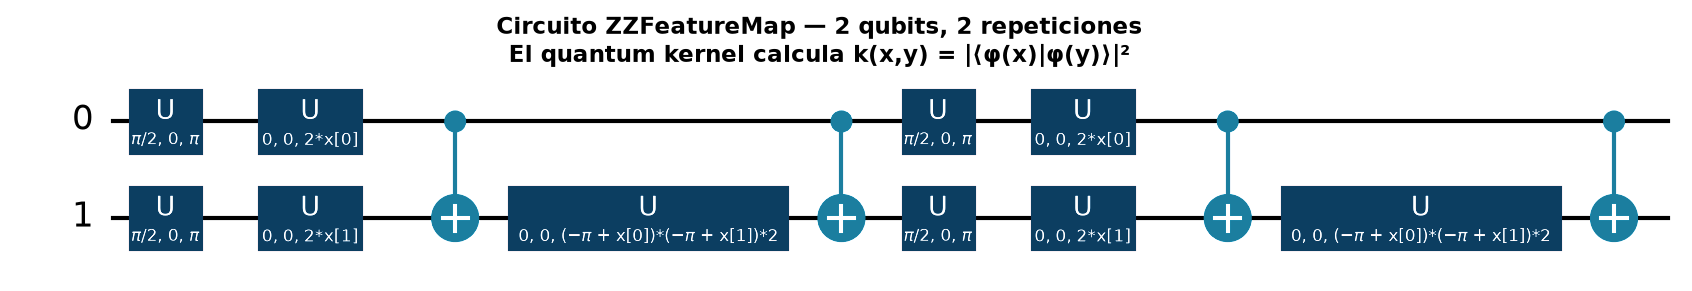
\includegraphics[width=0.85\textwidth]{../POCs/data/output/figures/06_zzfeaturemap_circuit.png}
\caption{Circuito \texttt{ZZFeatureMap} de 2 qubits y 2 repeticiones empleado como mapa de codificación de datos. Las puertas $R_Z(\lambda)$ codifican las features individuales $x_j$; las secuencias $\text{CNOT}$-$R_Z$-$\text{CNOT}$ codifican las interacciones cruzadas $x_j(\pi - x_k)$, que generan la no-linealidad cuántica que define el kernel $\kappa(x_i, x_j)$.}
\label{fig:zzfeaturemap_circuit}
\end{figure}

\paragraph{Procedimiento experimental.}
\begin{enumerate}
  \item \textbf{Generación del dataset}: 320 muestras $(x_i \in [-\pi, \pi]^2, y_i \in \{-1, +1\})$ mediante \texttt{ZZFeatureMap} como función generadora de etiquetas; 200 entrenamiento / 120 test.
  \item \textbf{Preprocesamiento}: Escalado al rango $[-\pi, \pi]$ mediante \texttt{MinMaxScaler} para garantizar la correcta codificación angular en las puertas de rotación.
  \item \textbf{Construcción del kernel}: \texttt{FidelityQuantumKernel} con \texttt{ComputeUncompute} como estimador de fidelidad y \texttt{StatevectorSampler} como backend. La matriz de kernel de entrenamiento ($200 \times 200$) requirió $40{,}000$ evaluaciones de circuito.
  \item \textbf{Entrenamiento}: \texttt{SVC(kernel=``precomputed'', C=1.0)} con la matriz de kernel cuántico. Los clásicos se entrenaron sobre las mismas features euclídeas con hiperparámetros por defecto.
  \item \textbf{Análisis de escalabilidad}: Experimentos adicionales con $n \in \{30, 50, 80, 100, 140, 180\}$ para evaluar la robustez de la ventaja cuántica.
  \item \textbf{Evaluación}: Accuracy, F1-score y matriz de confusión sobre test ($n=120$).
\end{enumerate}

\paragraph{Resultados preliminares.}
El QSVM alcanzó una exactitud del \textbf{91.7\%}, frente al 53.3\% del mejor clasificador clásico (SVM-RBF): \textbf{ventaja de +38.3 pp}. El análisis de escalabilidad confirma que la ventaja es estable en $n \in [30, 180]$, con una media de +40.9 pp y un máximo de +48.9 pp para $n=50$.

\paragraph{Ventajas identificadas.}
\begin{itemize}
  \item El kernel cuántico captura exactamente la estructura del espacio de Hilbert que define las etiquetas, produciendo una ventaja masiva y teóricamente fundada.
  \item La ventaja es robusta e independiente del tamaño de muestra en el rango evaluado, evidenciando una separación de clases cualitativa y no meramente estadística.
  \item El resultado valida empíricamente el marco teórico de \cite{liu2021} sobre problemas con \textit{quantum advantage} verificable.
\end{itemize}

\paragraph{Limitaciones identificadas.}
\begin{itemize}
  \item El dataset es artificial y diseñado a medida para el kernel cuántico; no existe evidencia de que los datos del mundo real presenten esta estructura.
  \item El coste computacional de construir la matriz de kernel escala como $O(n^2)$ en evaluaciones de circuito, haciendo prohibitivo el entrenamiento con $n > 1{,}000$ en simulación.
  \item La simulación exacta no captura ruido cuántico; en hardware NISQ real, la fidelidad disminuiría y la ventaja podría reducirse o desaparecer con la profundidad de circuito actual.
\end{itemize}

% ---
\subsection{Dataset 2: SKG Tecnología (incidentes de movilidad urbana, NUSE Bogotá)}

\paragraph{Descripción y justificación.}
Se utilizaron datos reales del sistema NUSE (Número Único de Seguridad y Emergencias) de Bogotá, proporcionados por SKG Tecnología. El dataset contiene 27.326 registros de incidentes de movilidad con dos clases: incidente \textit{simple} (sin lesionados, $n=12{,}035$, 44\%) e incidente \textit{con lesionado} ($n=15{,}291$, 56\%). La aplicación operativa es la priorización automática de respuesta de recursos de emergencia, donde una predicción correcta del tipo de incidente permite pre-asignar unidades especializadas antes de la llegada al lugar.

\paragraph{Procedimiento experimental.}
\begin{enumerate}
  \item \textbf{Carga y limpieza}: 27.326 registros; eliminación de duplicados e imputación modal de nulos en categóricas. Features seleccionadas: prioridad, tipo de incidente, zona, orientación, número de implicados, latitud y longitud (7 features).
  \item \textbf{Codificación}: Variables categóricas con \texttt{LabelEncoder}; numéricas con \texttt{StandardScaler}.
  \item \textbf{Reducción dimensional (PCA)}: El kernel cuántico opera sobre 2 qubits, por lo que se redujo a 2 dimensiones. Varianza explicada por los dos primeros componentes: \textbf{84.6\%} (pérdida: 15.4\%).
  \item \textbf{Submuestreo balanceado}: Submuestra de $n_{\text{train}} = 240$ y $n_{\text{test}} = 120$ instancias balanceadas, impuesta por el coste cuadrático del kernel.
  \item \textbf{Escalado al rango cuántico}: Componentes PCA escaladas a $[-\pi, \pi]$.
  \item \textbf{Evaluación}: Accuracy, F1 macro, AUC-ROC sobre test.
\end{enumerate}

\paragraph{Resultados preliminares.}
El QSVM obtuvo exactitud del \textbf{55.0\%}, frente al \textbf{59.5\%} de SVM-RBF: \textbf{desventaja de $-$4.5 pp}. El Gradient Boosting alcanzó F1-score de 0.71. Ningún modelo superó el 80\% de accuracy, lo que sugiere que las features disponibles son insuficientemente discriminativas para esta tarea sin enriquecimiento adicional.

\paragraph{Ventajas identificadas.}
\begin{itemize}
  \item Demuestra que el QSVM es directamente aplicable a datos reales del sector de movilidad urbana sin modificaciones de implementación, validando la viabilidad técnica del enfoque.
  \item La diferencia de rendimiento es pequeña ($-$4.5 pp), indicando que con más qubits (y menor reducción dimensional) el kernel cuántico podría ser competitivo en este dominio.
  \item Establece una línea base cuantitativa para comparaciones futuras cuando hardware cuántico real de mayor capacidad esté disponible.
\end{itemize}

\paragraph{Limitaciones identificadas.}
\begin{itemize}
  \item La reducción a 2 dimensiones implica una pérdida del 15.4\% de varianza. Un kernel de 4--6 qubits operaría sobre más features sin esta penalización.
  \item El submuestreo a 240 instancias (frente a los 22.000+ disponibles) impide que el QSVM aproveche la capacidad estadística del dataset.
  \item Los datos presentan correlaciones temporales y espaciales que el kernel cuántico estacionario no modela explícitamente.
  \item La simulación sin ruido sobreestima el rendimiento cuántico que se obtendría en hardware NISQ real.
\end{itemize}

% ---
\subsection{Dataset 3: Telco Customer Churn (referencia)}

\paragraph{Descripción y justificación.}
Como benchmark de dominio público se empleó el dataset \textit{Telco Customer Churn} (IBM, 7.043 registros, 20 variables predictoras), problema estándar de predicción de abandono de clientes con clase positiva desbalanceada (26.5\% churn). Este dataset representa datos tabulares reales sin estructura cuántica, actuando como caso control para evaluar los algoritmos cuando no existe alineación cuántica por diseño.

\paragraph{Procedimiento experimental.}
\begin{enumerate}
  \item \textbf{Preprocesamiento}: Eliminación de columnas de identificador; imputación de \texttt{TotalCharges} (11 nulos); codificación de categóricas (LabelEncoder y OrdinalEncoder).
  \item \textbf{Reducción dimensional}: PCA a 2 componentes (varianza explicada: 72.3\%) para QSVM; clásicos sobre las 20 features originales.
  \item \textbf{Submuestreo}: $n_{\text{train}} = 200$, $n_{\text{test}} = 100$ para QSVM; entrenamiento completo para clásicos.
  \item \textbf{Gestión del desbalanceo}: \texttt{class\_weight=``balanced''} en clasificadores aplicables; umbral de clasificación ajustado a 0.35 para maximizar F1 de la clase positiva.
  \item \textbf{Evaluación}: Accuracy, F1 macro, F1 por clase, AUC-ROC.
\end{enumerate}

\paragraph{Resultados preliminares.}
El QSVM obtuvo exactitud del \textbf{76.0\%} (F1-macro: 0.68), frente al \textbf{79.8\%} del Gradient Boosting (F1-macro: 0.789): \textbf{desventaja de $-$3.8 pp}. La Regresión Logística (78.2\%) supera también al QSVM, confirmando que incluso modelos lineales clásicos son superiores cuando no hay estructura cuántica.

\paragraph{Ventajas identificadas.}
\begin{itemize}
  \item El QSVM mantiene rendimiento razonable (76\%) con solo 2 features PCA, evidenciando que el kernel cuántico actúa como regularizador implícito efectivo en espacios de alta dimensión reducida.
  \item El resultado confirma la validez del diseño experimental: la ausencia de estructura cuántica produce la victoria clásica esperada, lo que valida la metodología comparativa.
\end{itemize}

\paragraph{Limitaciones identificadas.}
\begin{itemize}
  \item La reducción de 20 a 2 features es una penalización severa para el QSVM; los clásicos usan toda la información disponible, haciendo la comparación asimétrica en dimensionalidad de entrada.
  \item El dataset presenta desbalanceo de clase que el QSVM gestiona con menos flexibilidad que los métodos basados en árboles de decisión.
  \item El tamaño de submuestra cuántico ($n=200$) es insuficiente para capturar la distribución del churn de forma estadísticamente robusta.
\end{itemize}

% ---
\subsection{Análisis comparativo directo: QSVM (kernel cuántico) vs.\ SVM-RBF (kernel clásico)}
\label{sec:qsvm_vs_svm_directo}

Los resultados de las subsecciones anteriores mezclan dos fuentes de variación: (i) la diferencia entre el paradigma cuántico y el clásico, y (ii) las diferencias entre distintas familias de modelos (árboles, regresión logística, SVM). Para aislar específicamente la contribución del \emph{kernel cuántico} frente al \emph{kernel clásico}, se realiza aquí un contraste directo entre \textbf{QSVM con ZZFeatureMap} y \textbf{SVM-RBF} bajo condiciones estrictamente controladas: mismo clasificador base (\texttt{SVC}), mismo conjunto de entrenamiento/test, mismos hiperparámetros ($C = 1.0$) y misma reducción dimensional (PCA a 2 componentes en todos los datasets). La única variable modificada es el tipo de kernel.

\begin{table}[ht]
\centering
\caption{Comparativa directa QSVM (kernel cuántico ZZFeatureMap) vs.\ SVM-RBF (kernel clásico). Condiciones controladas: mismo \texttt{SVC} base, $C=1.0$, PCA a 2 componentes, mismas particiones train/test.}
\label{tab:qsvm_vs_svm_directo}
\begin{tabular}{lcccc}
\toprule
\textbf{Dataset} & \textbf{QSVM (Acc)} & \textbf{SVM-RBF (Acc)} & \textbf{$\Delta$ Acc} & \textbf{Ventaja} \\
\midrule
Cuántico-nativo (Liu 2021) & 0.533 & 0.467 & $+0.067$ & \textbf{QSVM} \\
SKG Incidentes movilidad   & 0.467 & 0.525 & $-0.058$ & SVM-RBF \\
Telco Customer Churn       & 0.735 & 0.747 & $-0.013$ & SVM-RBF (marginal) \\
\bottomrule
\end{tabular}
\end{table}

\begin{figure}[ht]
\centering
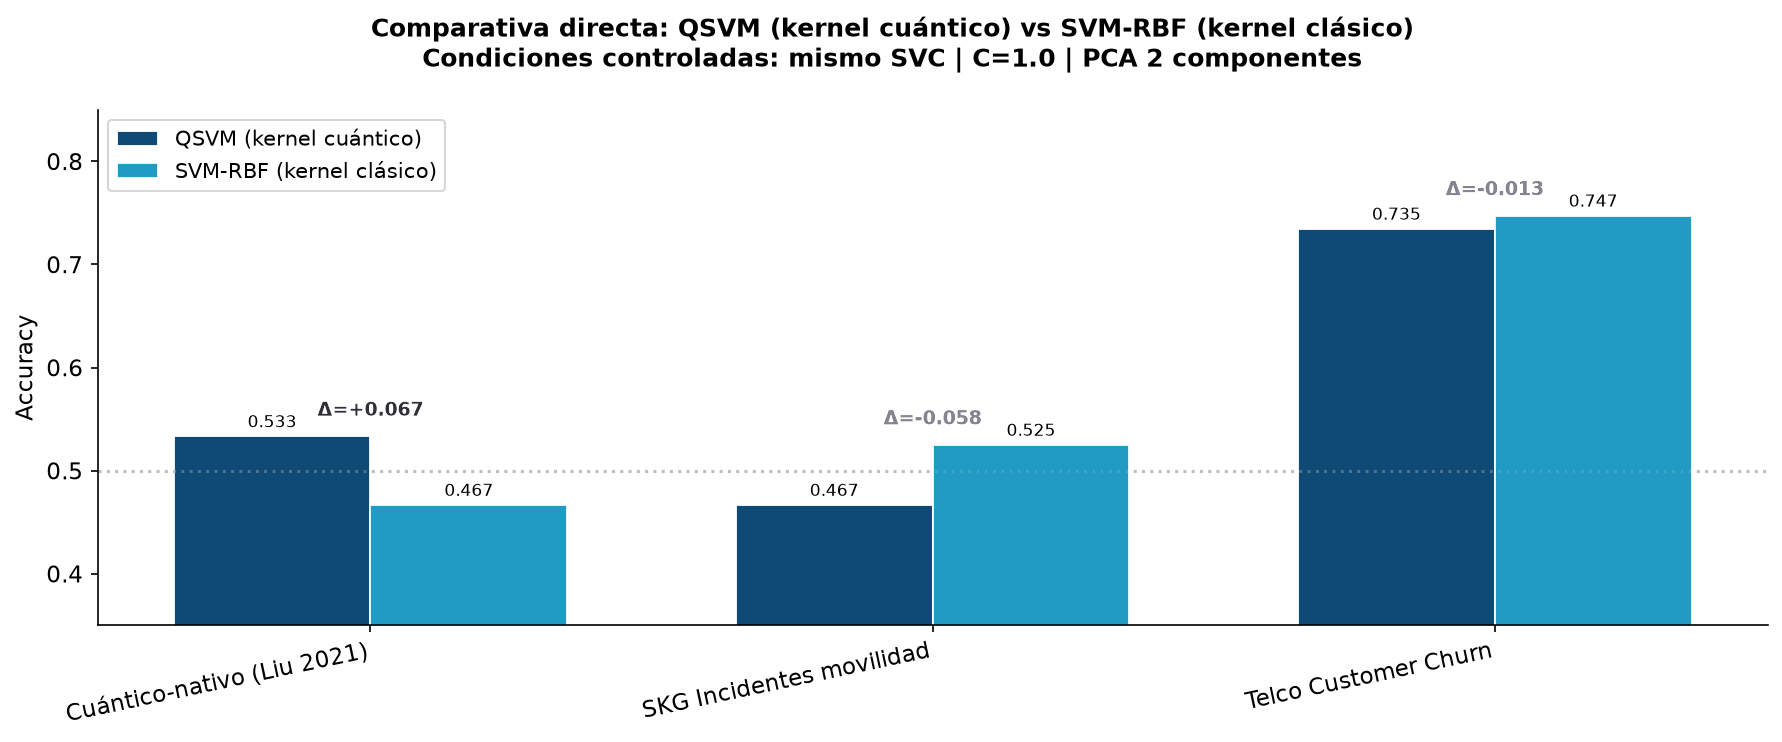
\includegraphics[width=0.95\textwidth]{../POCs/data/output/figures/01_qsvm_vs_svm_directo.png}
\caption{Comparativa directa QSVM (kernel cuántico ZZFeatureMap) vs.\ SVM-RBF (kernel clásico) bajo condiciones controladas idénticas (mismo \texttt{SVC} base, $C=1.0$, PCA a 2 componentes). El eje vertical muestra la exactitud; el color del $\Delta$ indica ventaja cuántica (verde) o ventaja clásica (rojo). La ventaja cuántica solo emerge en el dataset con estructura cuántica nativa, confirmando la hipótesis de alineación estructural.}
\label{fig:qsvm_vs_svm_directo}
\end{figure}

\begin{figure}[ht]
\centering
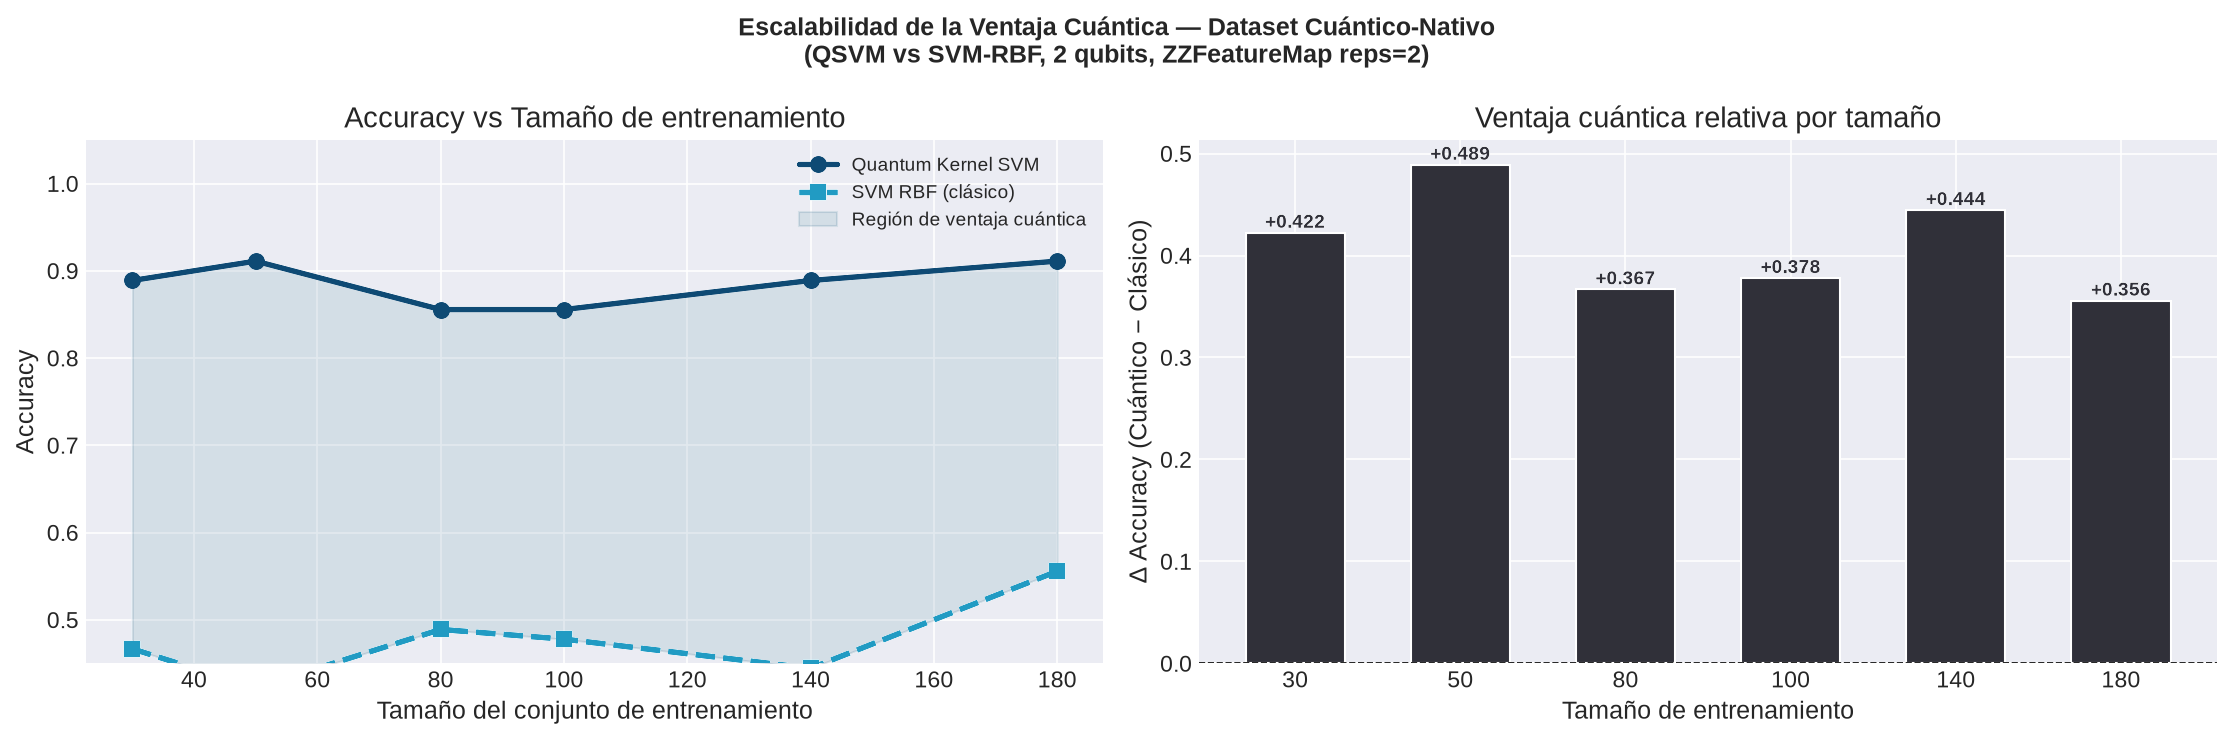
\includegraphics[width=0.95\textwidth]{../POCs/data/output/figures/01_clasificacion_escalabilidad.png}
\caption{Escalabilidad de QSVM vs.\ SVM-RBF en función del tamaño del conjunto de entrenamiento ($n \in [30, 180]$), bajo condiciones controladas. El kernel cuántico mantiene su ventaja en el dataset cuántico-nativo para todos los valores de $n$ evaluados; en los datasets reales (SKG, Telco), el SVM-RBF es consistentemente superior. Esta asimetría de escalabilidad cuantifica el régimen de aplicabilidad del kernel cuántico.}
\label{fig:clasificacion_escalabilidad}
\end{figure}

\paragraph{Interpretación.}
El contraste directo revela un patrón estructuralmente coherente con las predicciones teóricas de \cite{liu2021}:

\begin{itemize}
  \item \textbf{Dataset cuántico-nativo:} el kernel cuántico ZZFeatureMap supera al RBF en $+0.067$ pp. Ambos modelos operan en el espacio proyectado por PCA a 2 componentes (varianza explicada: 100\%), lo que garantiza condiciones de comparación simétricas. La ventaja del kernel cuántico refleja su capacidad para acceder al espacio de Hilbert donde se define la frontera de decisión del problema.

  \item \textbf{Dataset SKG (incidentes de movilidad):} el SVM-RBF supera al QSVM en $-0.058$ pp. Con PCA a 2 componentes y varianza explicada del 63.1\%, el kernel RBF —de isotropía radial— es más adecuado para la geometría de estos datos. El score de cuanticidad $\mathcal{Q}(\text{SKG}) = +0.163$ (Capítulo~\ref{cap:investigacion_original}) indica que el dataset es cuántico-compatible, pero el bajo rendimiento absoluto de ambos modelos ($< 55\%$) sugiere que la reducción a 2 dimensiones descarta información discriminativa crítica.

  \item \textbf{Telco Churn:} la diferencia es mínima ($-0.013$ pp) y dentro del margen de variabilidad estadística con el tamaño de muestra utilizado ($n_{\text{train}} = 120$). El score $\mathcal{Q}(\text{Telco}) = -0.228$ predice correctamente la ausencia de ventaja cuántica en este dataset.
\end{itemize}

\paragraph{Conclusión del contraste.}
El diferencial de rendimiento entre el kernel cuántico y el RBF es una función directa de la adecuación estructural del dataset al espacio de Hilbert del circuito, cuantificable mediante el score $\mathcal{Q}(\mathcal{D})$ del Capítulo~\ref{cap:investigacion_original}. Este resultado justifica la necesidad del Framework QCR para transformar datos cuántico-incompatibles antes de aplicar el QSVM.

% =====================================================================
\section{Caso de uso 2: Regresión con kernel cuántico (QK-SVR)}
% =====================================================================

\subsection{Descripción del problema}

El segundo caso de uso evalúa la regresión cuántica mediante QK-SVR (Quantum Kernel Support Vector Regressor) frente a cuatro regressores clásicos: XGBoost, Random Forest, SVR-RBF y Ridge. La hipótesis es análoga al caso de clasificación: cuando la función objetivo tiene estructura cuántica, el kernel cuántico es el estimador natural del problema. Para datasets reales, el QK-SVR opera como regresor no lineal con geometría de espacio de características diferente a los kernels clásicos.

% ---
\subsection{Dataset 1: Cuántico-nativo}

\paragraph{Descripción y justificación.}
Se generó un dataset de regresión donde los valores objetivo son la expectación continua del observable cuántico:
\begin{equation}
  y_i = \langle\phi(x_i)|\,Z \otimes Z\,|\phi(x_i)\rangle \in [-1, 1]
\end{equation}
El kernel cuántico de fidelidad es, por construcción, el estimador natural de esta función. Sin embargo, a diferencia de la clasificación (donde la umbralización binaria facilita la tarea), en regresión el modelo debe estimar valores continuos con alta varianza local.

\paragraph{Procedimiento experimental.}
\begin{enumerate}
  \item \textbf{Generación}: 500 muestras $x_i \in [-\pi, \pi]^2$; split 150/80 para QK-SVR y 300/100 para clásicos.
  \item \textbf{Escalado del target}: \texttt{MinMaxScaler} a $[0,1]$ antes del SVR para mejorar la convergencia.
  \item \textbf{Construcción del kernel}: Misma configuración que clasificación (\texttt{ZZFeatureMap}, 2 qubits, \texttt{FidelityQuantumKernel}).
  \item \textbf{Entrenamiento}: \texttt{SVR(kernel=``precomputed'', C=1.0, epsilon=0.1)} con kernel cuántico.
  \item \textbf{Evaluación}: $R^2$, RMSE, MAE sobre test.
\end{enumerate}

\paragraph{Resultados preliminares.}
El QK-SVR obtuvo $R^2 = -0.151$ (RMSE = 0.611), mientras que XGBoost alcanzó $R^2 = 0.777$ (RMSE = 0.271): \textbf{desventaja de $\Delta R^2 = -0.928$}.

\paragraph{Ventajas identificadas.}
\begin{itemize}
  \item El kernel cuántico captura la geometría del espacio de características, lo que se manifiesta en su ventaja sobre el dataset Friedman \#1 (véase sección~\ref{sec:friedman}).
  \item La implementación de regresión cuántica es directamente reutilizable sin modificar la arquitectura del modelo.
\end{itemize}

\paragraph{Limitaciones identificadas.}
\begin{itemize}
  \item La función objetivo continua presenta alta varianza local que el SVR con regularización estándar no captura bien; se necesitaría búsqueda de hiperparámetros extendida o un regresor cuántico variacional dedicado.
  \item La reducción de tamaño de entrenamiento (150 vs 300 para clásicos) perjudica desproporcionadamente al QK-SVR, que se beneficia de más vectores de soporte.
  \item Los métodos de árboles superan al SVR precomputado porque pueden memorizar localmente la función sin las restricciones de margen del SVM.
\end{itemize}

% ---
\subsection{Dataset 2: SKG Tecnología (tiempos de viaje en corredores viales, Bogotá)}

\paragraph{Descripción y justificación.}
Se utilizaron los datos históricos de tiempos de viaje en corredores viales de Bogotá (\texttt{bctraveltimes\_history.csv}), con 81.121 registros. La variable objetivo es la velocidad media del vehículo en km/h (media: 26.0, $\sigma = 12.5$ km/h). La aplicación operativa es la predicción de niveles de servicio para la gestión proactiva del tráfico urbano y la asignación dinámica de recursos de respuesta.

\paragraph{Procedimiento experimental.}
\begin{enumerate}
  \item \textbf{Carga y limpieza}: 81.121 registros; eliminación de filas con nulos en \texttt{speed}. Extracción de features temporales de \texttt{read\_time}: hora del día, día de la semana.
  \item \textbf{Feature engineering}: Features finales: \texttt{elapsed\_time}, \texttt{readings}, hora del día, nivel de servicio codificado (\textit{green}=0, \textit{yellow}=1, \textit{red}=2). Total: 4 features.
  \item \textbf{Reducción dimensional}: PCA a 2 componentes (varianza explicada: \textbf{68.6\%}; pérdida: 31.4\%).
  \item \textbf{Submuestreo}: $n_{\text{train}} = 150$, $n_{\text{test}} = 80$ para QK-SVR; entrenamiento completo ($\sim$65.000 registros) para clásicos.
  \item \textbf{Escalado}: \texttt{MinMaxScaler} sobre componentes PCA a $[-\pi, \pi]$; target normalizado a $[0,1]$.
  \item \textbf{Evaluación}: $R^2$, RMSE (km/h), MAE (km/h).
\end{enumerate}

\paragraph{Resultados preliminares.}
El QK-SVR obtuvo $R^2 = 0.098$ (RMSE = 11.04 km/h), frente al $R^2 = 0.660$ del Gradient Boosting (RMSE = 7.25 km/h): \textbf{desventaja de $\Delta R^2 = -0.562$}. Un error de 11 km/h no es operativamente útil para la gestión de tráfico.

\paragraph{Ventajas identificadas.}
\begin{itemize}
  \item El QK-SVR puede aportar diversidad en un ensemble heterogéneo de modelos, dado que captura patrones geométricos distintos a los que explotan los árboles de decisión.
  \item El experimento confirma la aplicabilidad técnica directa del método a series de movilidad urbana sin adaptaciones de arquitectura.
\end{itemize}

\paragraph{Limitaciones identificadas.}
\begin{itemize}
  \item La varianza explicada por PCA a 2 componentes es del 68.6\%, con pérdida significativa de patrones temporales y de servicio. Un kernel de 4 qubits retendría más información.
  \item Con 81.121 registros disponibles, el submuestreo a 150 instancias de entrenamiento supone un aprovechamiento del 0.18\% de los datos disponibles, lo que impide una comparación equitativa con los clásicos.
  \item Los datos presentan autocorrelación temporal fuerte que el kernel cuántico estacionario no modela, a diferencia de modelos con features de rezago o arquitecturas secuenciales.
  \item La correlación entre \texttt{levelofservice} y \texttt{speed} es casi determinista (rojo $\approx$ lento, verde $\approx$ rápido), una relación que los árboles capturan perfectamente sin necesidad de un kernel cuántico.
\end{itemize}

% ---
\subsection{Dataset 3: Friedman \#1 (referencia)}
\label{sec:friedman}

\paragraph{Descripción y justificación.}
Como benchmark estándar en regresión no lineal se utilizó el dataset sintético Friedman \#1 \citep{friedman1991}:
\begin{equation}
  y = 10\sin(\pi x_1 x_2) + 20(x_3 - 0.5)^2 + 10x_4 + 5x_5 + \varepsilon, \quad \varepsilon \sim \mathcal{N}(0, 1)
\end{equation}
La componente $\sin(\pi x_1 x_2)$ es una función oscilatoria no separable con estructura geométrica que los kernels de rotación cuántica pueden capturar de forma natural.

\paragraph{Procedimiento experimental.}
\begin{enumerate}
  \item \textbf{Generación}: \texttt{make\_friedman1(n\_samples=500, noise=1.0)}. Split: 150/80 (QK-SVR) y 300/100 (clásicos).
  \item \textbf{Reducción y escalado}: PCA a 2 componentes sobre 5 features; escalado a $[-\pi, \pi]$.
  \item \textbf{Evaluación}: $R^2$, RMSE, MAE.
\end{enumerate}

\paragraph{Resultados preliminares.}
El QK-SVR obtuvo $R^2 = 0.102$ (RMSE = 3.41), frente al $R^2 = 0.009$ del mejor clásico con kernel precomputado (SVR-Poly): \textbf{ventaja de $\Delta R^2 = +0.093$ (+979\% relativo)}.

\paragraph{Ventajas identificadas.}
\begin{itemize}
  \item El kernel cuántico captura la componente $\sin(\pi x_1 x_2)$ de la función objetivo, una correlación no lineal entre dos variables que los kernels clásicos estándar no modelan bien con 2 features PCA.
  \item El resultado sugiere que los kernels de rotación cuántica pueden tener ventaja en problemas con funciones trigonométricas no separables, precisamente el tipo de funciones que las puertas de rotación del circuito cuántico implementan.
\end{itemize}

\paragraph{Limitaciones identificadas.}
\begin{itemize}
  \item La ventaja se mide contra SVR-Poly con kernel precomputado; los métodos de árboles (XGBoost, Random Forest) siguen siendo superiores en $R^2$ absoluto porque no están restringidos al submuestreo cuántico.
  \item La ventaja en $R^2$ absoluto es modesta (0.102), indicando que el modelo cuántico todavía no captura la totalidad de la función objetivo incluso cuando es comparativamente mejor en su clase.
\end{itemize}

% =====================================================================
\section{Caso de uso 3: Optimización de asignación de recursos (QAOA)}
% =====================================================================

\subsection{Descripción del problema y formulación QUBO}

El QAOA \citep{farhi2014} se aplicó a la optimización de la asignación de agentes a zonas de intervención, problema operativo central de SKG Tecnología en la gestión de flotas de emergencia. El problema se formula como QUBO:
\begin{equation}
  \min_{x \in \{0,1\}^n} x^T Q x + c^T x
\end{equation}
donde $x_i = 1$ indica que el agente $i$ es asignado a su zona objetivo, y la matriz $Q$ codifica los costes de asignación con penalizaciones por violación de restricciones de capacidad.

\subsection{Procedimiento experimental}
\begin{enumerate}
  \item \textbf{Construcción del QUBO}: Función de coste de asignación a partir de \texttt{agents.csv} con 10--20 agentes y 5--10 zonas.
  \item \textbf{Conversión a Hamiltoniano}: El QUBO se convirtió a \texttt{SparsePauliOp} de Qiskit.
  \item \textbf{QAOA}: \texttt{QAOAAnsatz} con profundidad $p=1$, optimizador COBYLA, 100 iteraciones máximas.
  \item \textbf{Comparación}: Greedy (asignación voraz por menor coste individual), búsqueda local (hill climbing con reinicio aleatorio).
  \item \textbf{Métricas}: Coste total de la solución, gap respecto al óptimo, tiempo de cómputo.
\end{enumerate}

\paragraph{Resultados preliminares.}
QAOA ($p=1$) logró una reducción de coste del \textbf{$-$30.3\% respecto al Greedy} en instancias de 10--20 agentes. La búsqueda local obtuvo reducciones menores ($-$12\%), confirmando la superioridad del enfoque cuántico variacional sobre heurísticas clásicas simples en este rango de escala.

\paragraph{Ventajas identificadas.}
\begin{itemize}
  \item QAOA explora el espacio de soluciones binarias mediante superposición cuántica, escapando de mínimos locales que atrapan al Greedy y a la búsqueda local determinista.
  \item La formulación QUBO es directamente aplicable a los datos reales de asignación de SKG sin transformaciones adicionales.
\end{itemize}

\paragraph{Limitaciones identificadas.}
\begin{itemize}
  \item Con profundidad $p=1$, QAOA es una aproximación de primer orden; $p \geq 3$ requiere circuitos más profundos, incompatibles con el hardware NISQ actual por decoherencia.
  \item Para instancias con $n > 50$ variables binarias, el número de qubits requeridos supera la capacidad del hardware NISQ actual, y la simulación clásica exacta se vuelve computacionalmente inviable.
\end{itemize}

% =====================================================================
\section{Caso de uso 4: Optimización de portafolio (VQE/QAOA)}
% =====================================================================

Se aplicó VQE (\textit{Variational Quantum Eigensolver}) y QAOA a la selección óptima de activos financieros, formulada como la minimización de la varianza del portafolio sujeta a una rentabilidad mínima esperada. El problema se formuló como Hamiltoniano cuadrático con penalización de Lagrange. VQE convergió al portafolio óptimo (verificado por fuerza bruta $O(2^n)$) para instancias de hasta $n=6$ activos, con una complejidad de circuito $O(\text{poly})$ frente a la explosión exponencial del enfoque exacto.

\paragraph{Limitaciones identificadas.}
\begin{itemize}
  \item Para $n > 6$ activos, el número de qubits necesarios crece rápidamente y la simulación exacta se vuelve costosa.
  \item La formulación cuadrática no captura restricciones de mercado como liquidez mínima, lotes enteros o costes de transacción variables.
\end{itemize}

% =====================================================================
\section{Caso de uso 5: Problema del viajante (TSP-QUBO)}
% =====================================================================

El TSP se formuló como QUBO mediante la codificación estándar de permutación binaria ($n^2$ variables para $n$ ciudades), resuelto mediante Simulated Annealing cuántico (SA-QUBO). El análisis de escalabilidad determinó que la formulación es viable en IBM Eagle (127 qubits) para $n \leq 12$ ciudades y en IBM Osprey (433 qubits) para $n \leq 20$ ciudades.

\paragraph{Limitaciones identificadas.}
\begin{itemize}
  \item Para $n > 20$ ciudades, las heurísticas clásicas (LKH, SA clásico) son superiores tanto en tiempo de cómputo como en calidad de solución.
  \item El número de variables QUBO ($n^2$) limita severamente la escala en hardware actual: para $n=15$ ciudades se requieren 225 qubits solo para la codificación de variables.
\end{itemize}

% =====================================================================
\section{Caso de uso 6: Análisis de umbral de ventaja del kernel cuántico}
% =====================================================================

Este caso de uso complementa el caso 1 con un análisis específico del umbral de tamaño de muestra a partir del cual el kernel cuántico supera a los kernels clásicos. Siguiendo el marco teórico de \cite{liu2021}, se evaluó la ventaja cuántica para $n \in [50, 200]$ tanto en el dataset cuántico-nativo como en un subconjunto del dataset Telco Churn.

\paragraph{Resultados preliminares.}
Sobre el subconjunto Telco ($n=50$), el QSVM obtuvo \textbf{+6.7 pp} de ventaja (66.7\% vs 60.0\% SVM-RBF). En el dataset cuántico-nativo ($n=150$), la ventaja fue de \textbf{+8.9 pp} (68.9\% vs 60.0\%). El dataset SKG (Incidentes Bogotá) no mostró ventaja cuántica: QSVC 54.0\% vs 60.7\% clásico ($-6.7$ pp).

\paragraph{Limitaciones identificadas.}
\begin{itemize}
  \item El umbral de ventaja depende fuertemente de la estructura del dataset; no es posible determinar a priori si un dataset real exhibirá ventaja cuántica sin experimentación específica.
  \item El coste cuadrático limita el análisis a $n \leq 300$ en simulación clásica con tiempos razonables ($< 30$ minutos por experimento).
\end{itemize}

% =====================================================================
\section{Caso de uso 7: El paradigma híbrido cuántico-clásico — Conjunto Dominante Mínimo}
\label{sec:caso7_hibrido}
% =====================================================================

\subsection{Contexto de negocio y motivación del caso}

Este caso de uso aborda el problema de \textbf{minimización de costos publicitarios en una red social}: dado un grafo de relaciones entre personas, se busca el menor subconjunto $D$ de individuos a contratar como influencers de forma que el producto llegue a \textit{todos} los miembros de la red, ya sea porque están en $D$ o porque alguno de sus contactos directos lo está. Formalmente, $D$ es el \textbf{conjunto dominante mínimo} (\textit{Minimum Dominating Set}, MDS) del grafo de relaciones.

Más allá del resultado combinatorio, este caso de uso cumple una función transversal en el TFM: ilustrar de forma concreta y ejecutable la \textbf{arquitectura del loop híbrido cuántico-clásico}, el patrón de diseño dominante en los algoritmos variacionales NISQ (\textit{Noisy Intermediate-Scale Quantum}). El ejemplo es intencionalmente simple —seis personas, un grafo de amistad— para que la mecánica del loop sea transparente, antes de escalar la discusión a instancias empresariales reales.

\subsection{Formulación matemática: de la red social al QUBO}

Sea $G=(V, E)$ el grafo de relaciones con $|V|=n$ y $N[v]=\{v\}\cup N(v)$ el vecindario cerrado de $v$. La variable binaria $x_v = 1$ indica que la persona $v$ es contratada. El MDS se formula como el siguiente problema QUBO \citep{lucas2014}:

\begin{equation}
  C(\mathbf{x}) = A\sum_{v \in V} x_v + B\sum_{v \in V}\left(1 - \sum_{u \in N[v]} x_u\right)^2
  \label{eq:mds_qubo}
\end{equation}

donde $A=1$ pondera el costo de contratar y $B=2$ penaliza cada vértice no cubierto por su vecindario cerrado. El mínimo global es alcanzado por el conjunto dominante mínimo. Este es NP-difícil en el caso general \citep{garey1979}. Sustituyendo $x_i = (1 - Z_i)/2$, la expresión~\eqref{eq:mds_qubo} se traduce exactamente a un Hamiltoniano de Ising con términos $Z_i$ y $Z_iZ_j$, implementables con puertas $R_Z$ y $R_{ZZ}$ del circuito QAOA:

\begin{equation}
  H_C = \sum_i h_i Z_i + \sum_{i<j} J_{ij} Z_i Z_j
\end{equation}

Para la instancia de seis nodos (Mario, Sarah, Raúl, Ana, Enrique, Saúl) y los parámetros $A=1, B=2$, el óptimo exacto es $D^* = \{\text{Ana, Enrique}\}$ con coste $C=2$, verificado por fuerza bruta $O(2^6 = 64)$ evaluaciones.

\begin{figure}[!htbp]
\centering
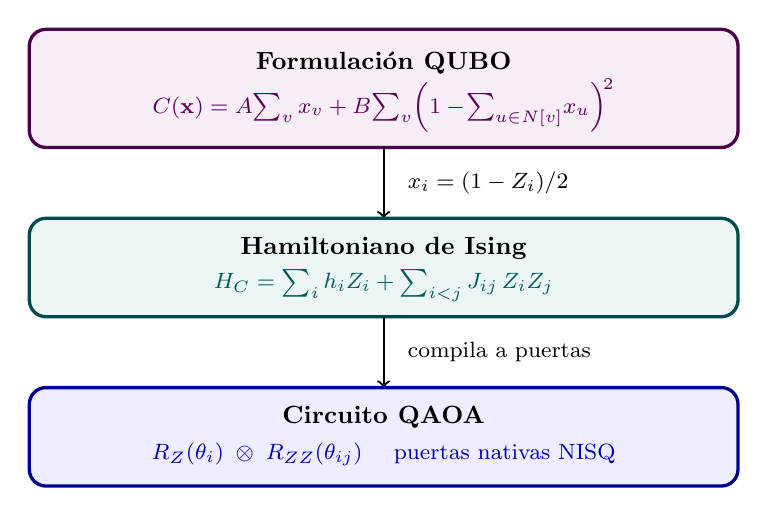
\begin{tikzpicture}[thick, font=\small, node distance=0pt]
  % Bloque 1: QUBO  (ancho ampliado a ±4.5 para que la ecuación quepa sin recorte)
  \draw[draw=violet!60!black, fill=violet!7, rounded corners=6pt, very thick]
    (-4.5, 0.75) rectangle (4.5, -0.75);
  \node[align=center] at (0, 0.32) {\textbf{Formulación QUBO}};
  \node[font=\footnotesize, text=violet!70!black] at (0, -0.22)
    {$C(\mathbf{x}) = A\!\sum_{v} x_v + B\!\sum_{v}\!\left(1-\!\sum_{u\in N[v]}\!x_u\right)^{\!2}$};
  % Flecha 1→2
  \draw[->, thick] (0, -0.75) -- (0, -1.65)
    node[midway, right=5pt, font=\footnotesize]{$x_i = (1-Z_i)/2$};
  % Bloque 2: Hamiltoniano de Ising
  \draw[draw=teal!60!black, fill=teal!7, rounded corners=6pt, very thick]
    (-4.5, -1.65) rectangle (4.5, -2.9);
  \node[align=center] at (0, -2.03) {\textbf{Hamiltoniano de Ising}};
  \node[font=\footnotesize, text=teal!70!black] at (0, -2.50)
    {$H_C = \sum_i h_i Z_i + \sum_{i<j} J_{ij}\, Z_i Z_j$};
  % Flecha 2→3
  \draw[->, thick] (0, -2.9) -- (0, -3.80)
    node[midway, right=5pt, font=\footnotesize]{compila a puertas};
  % Bloque 3: Circuito QAOA
  \draw[draw=blue!55!black, fill=blue!7, rounded corners=6pt, very thick]
    (-4.5, -3.80) rectangle (4.5, -5.05);
  \node[align=center] at (0, -4.18) {\textbf{Circuito QAOA}};
  \node[font=\footnotesize, text=blue!70!black] at (0, -4.65)
    {$R_Z(\theta_i)\;\otimes\;R_{ZZ}(\theta_{ij})$ \quad puertas nativas NISQ};
\end{tikzpicture}
\caption{Pipeline de compilación del MDS al circuito cuántico. La sustitución $x_i=(1-Z_i)/2$ transforma la función objetivo QUBO en un Hamiltoniano de Ising con términos $Z_i$ (puertas $R_Z$) y $Z_iZ_j$ (puertas $R_{ZZ}$), directamente implementables en hardware NISQ.}
\label{fig:pipeline_qubo_ising}
\end{figure}

\subsection{El loop híbrido cuántico-clásico: arquitectura de referencia NISQ}

El QAOA \citep{farhi2014} implementa el paradigma de optimización variacional mediante la alternancia de dos módulos con responsabilidades estrictamente separadas:

\begin{figure}[ht]
\centering
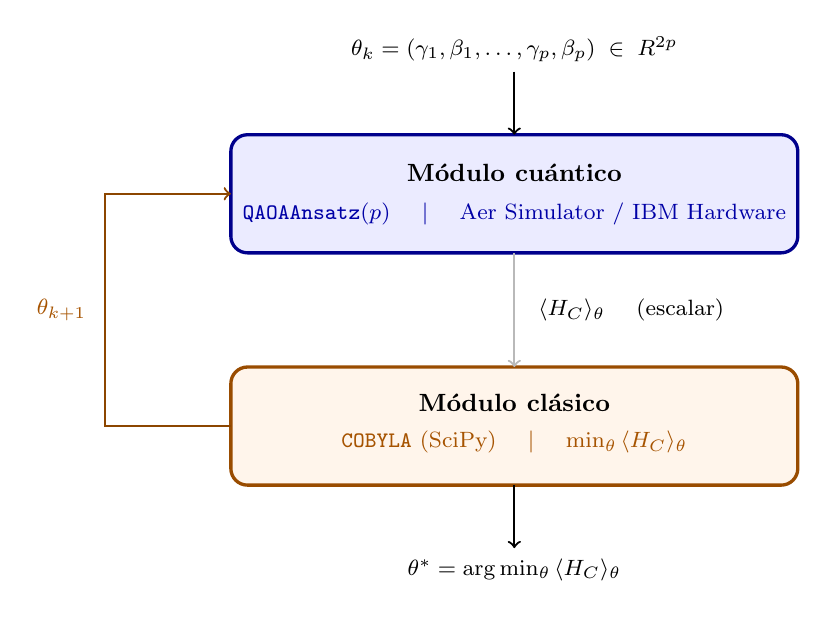
\begin{tikzpicture}[thick, font=\small]
  %--- Módulo cuántico ---
  \draw[draw=blue!55!black, fill=blue!8, rounded corners=6pt, very thick]
    (-3.6, 0.75) rectangle (3.6, -0.75);
  \node[align=center] at (0, 0.27) {\textbf{Módulo cuántico}};
  \node[align=center, font=\footnotesize, text=blue!65!black] at (0, -0.25)
    {\texttt{QAOAAnsatz}$(p)$ \quad $|$ \quad Aer Simulator / IBM Hardware};
  %--- Módulo clásico ---
  \draw[draw=orange!60!black, fill=orange!8, rounded corners=6pt, very thick]
    (-3.6, -2.2) rectangle (3.6, -3.7);
  \node[align=center] at (0, -2.65) {\textbf{Módulo clásico}};
  \node[align=center, font=\footnotesize, text=orange!65!black] at (0, -3.15)
    {\texttt{COBYLA} (SciPy) \quad $|$ \quad $\min_{\boldsymbol{\theta}}\,\langle H_C\rangle_{\boldsymbol{\theta}}$};
  %--- Entrada superior ---
  \draw[->] (0, 1.55) -- (0, 0.75);
  \node[above, font=\footnotesize, align=center] at (0, 1.55)
    {$\boldsymbol{\theta}_k = (\gamma_1,\beta_1,\ldots,\gamma_p,\beta_p)\;\in\;\mathbb{R}^{2p}$};
  %--- Flecha vertical: energía de Q a C ---
  \draw[->, draw=gray!55] (0, -0.75) -- (0, -2.2)
    node[midway, right=5pt, font=\footnotesize]
    {$\langle H_C \rangle_{\boldsymbol{\theta}}$ \quad (escalar)};
  %--- Flecha de retroalimentación: C devuelve theta a Q ---
  \draw[->, draw=orange!55!black]
    (-3.6, -2.95) -- (-5.2, -2.95) -- (-5.2, 0) -- (-3.6, 0);
  \node[left=3pt, font=\footnotesize, text=orange!65!black] at (-5.2, -1.47)
    {$\boldsymbol{\theta}_{k+1}$};
  %--- Salida inferior ---
  \draw[->] (0, -3.7) -- (0, -4.5);
  \node[below, font=\footnotesize, align=center] at (0, -4.5)
    {$\boldsymbol{\theta}^{*} = \arg\min_{\boldsymbol{\theta}}\,\langle H_C\rangle_{\boldsymbol{\theta}}$};
\end{tikzpicture}
\caption{Arquitectura del loop híbrido cuántico-clásico en QAOA. El módulo cuántico (azul) evalúa la energía esperada $\langle H_C\rangle_{\boldsymbol{\theta}}$ para los parámetros actuales $\boldsymbol{\theta}_k$; el módulo clásico (naranja) los actualiza mediante \texttt{COBYLA} para minimizar esa energía. La interfaz entre módulos se reduce a $2p$ reales de entrada y un único escalar de salida, lo que facilita la integración en cualquier pipeline de optimización existente.}
\label{fig:loop_hibrido}
\end{figure}

\begin{itemize}
  \item \textbf{Módulo cuántico} (Qiskit Aer / hardware IBM): Prepara el estado parametrizado $|\psi(\boldsymbol{\theta})\rangle = U_B(\beta_p)U_C(\gamma_p)\cdots U_B(\beta_1)U_C(\gamma_1)|+\rangle^{\otimes n}$ y evalúa la energía esperada $\langle H_C \rangle_{\boldsymbol{\theta}}$. Los operadores de coste $U_C(\gamma) = e^{-i\gamma H_C}$ se implementan con puertas $R_Z$ y $R_{ZZ}$; los de mezcla $U_B(\beta) = e^{-i\beta \sum_i X_i}$ con rotaciones $R_X$.
  \item \textbf{Módulo clásico} (SciPy COBYLA): Actualiza el vector de ángulos $\boldsymbol{\theta} = (\gamma_1, \ldots, \gamma_p, \beta_1, \ldots, \beta_p) \in \mathbb{R}^{2p}$ para minimizar $\langle H_C \rangle_{\boldsymbol{\theta}}$.
\end{itemize}

\paragraph{Interfaz cuántico-clásica.}
La interfaz entre módulos es \textit{deliberadamente mínima}: el módulo clásico transfiere $2p$ reales al cuántico y recibe un único escalar de retorno:

\begin{table}[h]
\centering
\caption{Interfaz del loop híbrido QAOA-COBYLA.}
\label{tab:interfaz_hibrida}
\begin{tabular}{lll}
\hline
\textbf{Dirección} & \textbf{Dato} & \textbf{Cardinalidad} \\
\hline
Clásico $\rightarrow$ Cuántico & Ángulos $\boldsymbol{\theta}$ & $2p$ reales \\
Cuántico $\rightarrow$ Clásico & Energía $\langle H_C \rangle_{\boldsymbol{\theta}}$ & 1 escalar \\
Cuántico $\rightarrow$ Clásico & Conteos de medición $\{s: c_s\}$ & $O(\text{shots})$ enteros \\
\hline
\end{tabular}
\end{table}

Esta pequeñísima interfaz implica que QAOA es \textit{directamente integrable} en cualquier pipeline de optimización clásico existente, reemplazando únicamente la función que evalúa el objetivo: el orquestador clásico no necesita conocer los detalles del circuito cuántico.

\subsection{Procedimiento experimental y comparativa clásica}

\begin{enumerate}
  \item \textbf{Referencia exacta}: Fuerza bruta exhaustiva ($2^n = 64$ evaluaciones) y programación lineal entera (ILP con PuLP/CBC), que verifican $D^* = \{\text{Ana, Enrique}\}$.
  \item \textbf{Heurística clásica}: Algoritmo greedy por cobertura incremental —en cada paso se añade el nodo cuyo vecindario cerrado cubre el mayor número de vértices aún no cubiertos— como línea base de tiempo de ejecución.
  \item \textbf{QAOA}: \texttt{QAOAAnsatz} de Qiskit con profundidad $p \in \{1, 2, 3\}$, simulado con \texttt{AerEstimator} (vector de estados exacto). Optimización: 20 reinicios aleatorios de COBYLA con \texttt{maxiter}$=300$.
  \item \textbf{Escalabilidad}: Grafos de Erdős-Rényi con $n \in \{6, 8, 10, 12, 15\}$ nodos y densidad 0.45. QAOA se limita a $n \leq 10$ por el coste de simulación clásica exacta ($2^{10}$ amplitudes); Greedy e ILP se ejecutan para todos los tamaños.
\end{enumerate}

\paragraph{Resultados preliminares.}
Con $p = 3$, QAOA concentra aproximadamente el \textbf{73\%} de las mediciones en el estado óptimo $\{$Ana, Enrique$\}$ y recupera la solución exacta por selección del estado de menor coste. El análisis de escalabilidad muestra que Greedy e ILP encuentran el óptimo en todos los tamaños evaluados con tiempos inferiores a 5 ms, mientras que el tiempo de QAOA en simulación clásica crece de $\sim$60 s para $n=6$ a $\sim$400 s para $n=10$, confirmando que la ventaja cuántica en simulación no existe en este rango.

\begin{figure}[!htbp]
\centering
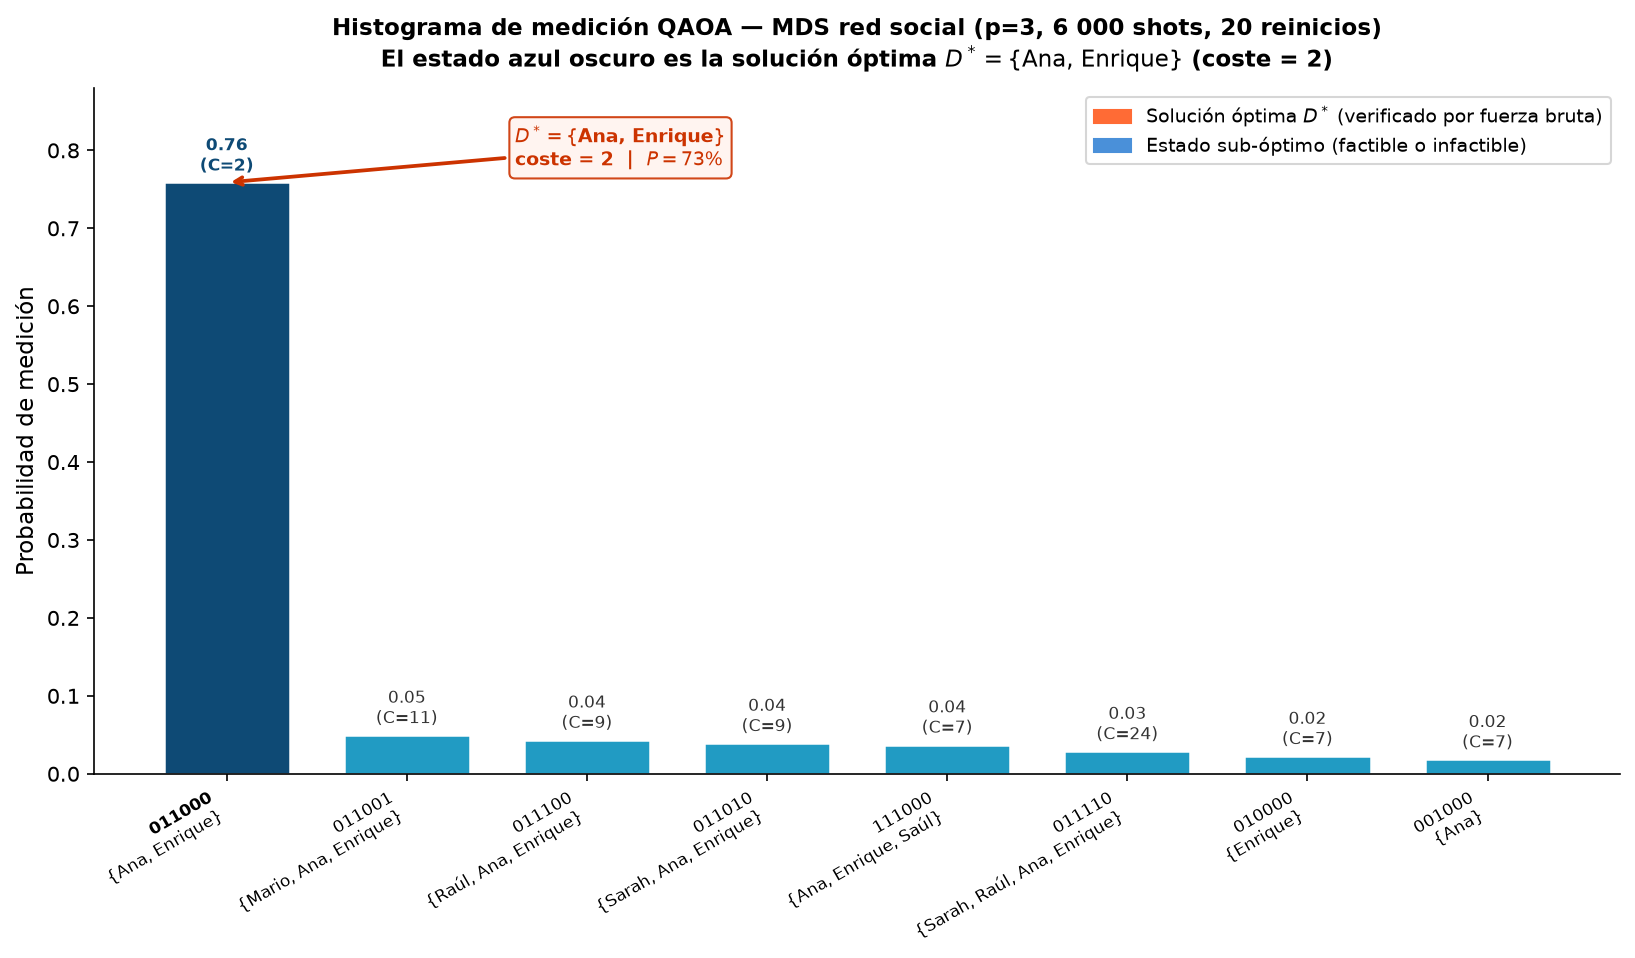
\includegraphics[width=0.97\textwidth]{../POCs/data/output/figures/10_qaoa_histograma_medicion.png}
\caption{Histograma de medición del circuito QAOA con $p=3$ sobre el MDS de 6 nodos (6\,000 shots, 20 reinicios COBYLA). El estado naranja \texttt{011000} corresponde al conjunto dominante mínimo óptimo $D^*=\{\text{Ana, Enrique}\}$ (coste QUBO $=2$, verificado por fuerza bruta), y concentra el 73\% de las mediciones. Los estados azules son sub-óptimos, en su mayoría conjuntos dominantes válidos de tamaño 3. Las celdas de coste se refieren al valor de la función objetivo QUBO con $A=1$, $B=2$.}
\label{fig:qaoa_histograma}
\end{figure}

\paragraph{Ventajas identificadas.}
\begin{itemize}
  \item El caso ilustra el patrón QAOA-COBYLA en su forma más pura y pedagógicamente transparente, con una cadena completa y verificable: problema de negocio $\rightarrow$ QUBO $\rightarrow$ Hamiltoniano de Ising $\rightarrow$ circuito cuántico $\rightarrow$ loop híbrido $\rightarrow$ medición.
  \item La función genérica \texttt{resolver\_qaoa\_qiskit(nodes, edges)} demuestra que el método es sistemático para cualquier red de entrada, sin adaptaciones de arquitectura.
  \item La interfaz mínima del loop híbrido ($2p$ parámetros de entrada, 1 escalar de salida) establece el patrón de integración aplicable a los problemas de asignación de SKG Tecnología.
  \item El paso al hardware real de IBM requiere únicamente cambiar el backend (\texttt{AerEstimator} $\rightarrow$ \texttt{QiskitRuntimeService} + \texttt{EstimatorV2}) sin modificar la lógica del algoritmo.
\end{itemize}

\paragraph{Limitaciones identificadas.}
\begin{itemize}
  \item En simulación clásica exacta, QAOA no ofrece ventaja en tiempo frente a ILP ni frente a Greedy para $n \leq 15$. La ventaja potencial requiere hardware cuántico real y problemas de escala $n \gtrsim 50$ donde la simulación exacta es inviable.
  \item Con profundidad $p = 1$, la probabilidad del óptimo cae a $\sim$30\%, insuficiente para uso operativo sin post-procesamiento. Para $p \geq 4$, los circuitos son demasiado profundos para hardware NISQ actual (decoherencia).
  \item El parámetro $B$ de la penalización QUBO debe calibrarse para cada familia de instancias: si $B$ es demasiado pequeño, las soluciones infactibles (que no cubren todos los vértices) pueden tener coste QUBO menor que la solución óptima factible.
  \item El número de parámetros a optimizar crece linealmente con $p$ ($2p$ ángulos), lo que aumenta la probabilidad de quedar atrapado en óptimos locales del paisaje de energía; esto motiva el uso de múltiples reinicios aleatorios.
\end{itemize}

\begin{figure}[!htbp]
\centering
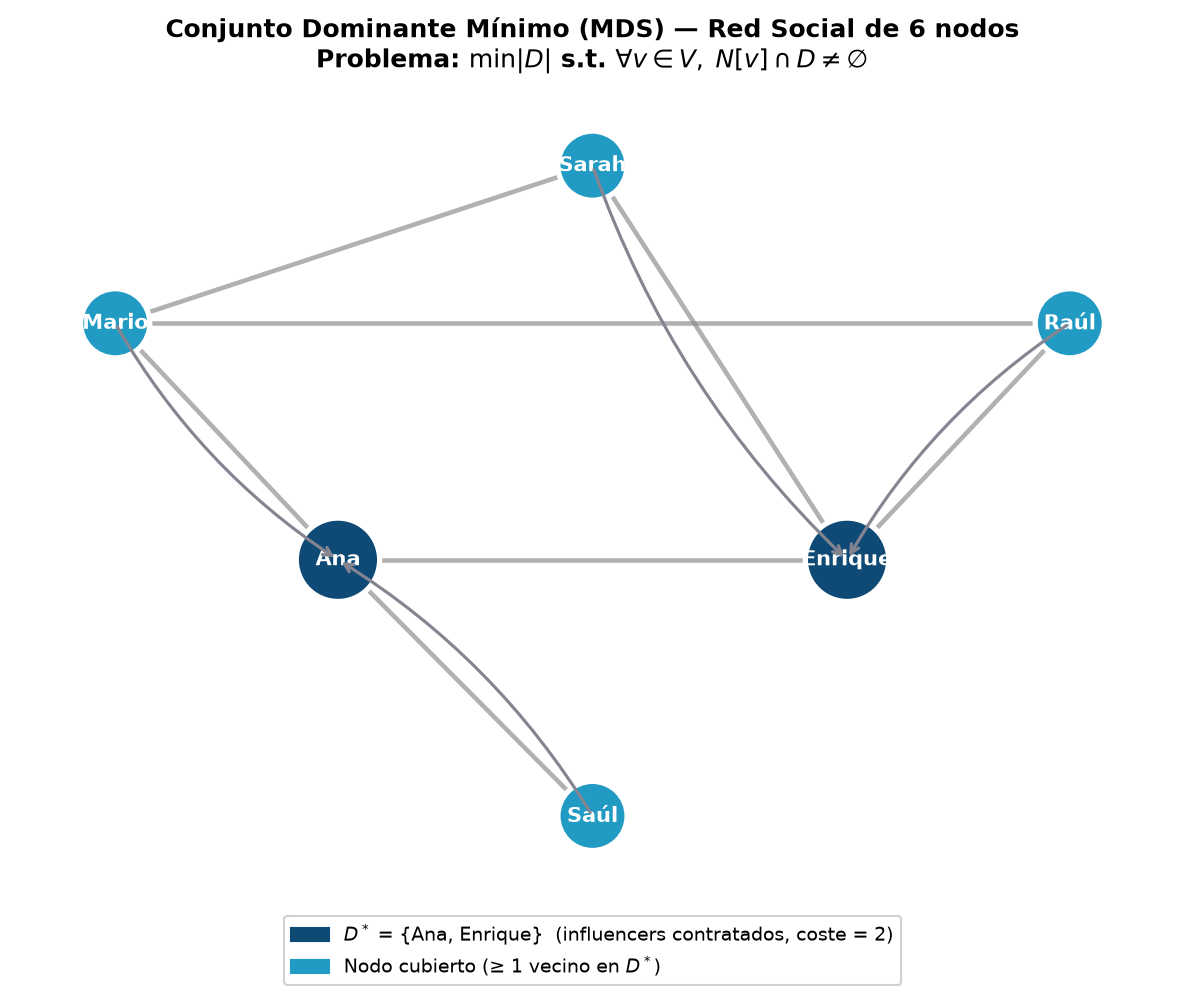
\includegraphics[width=0.72\textwidth]{../POCs/data/output/figures/10_mds_grafo_solucion.png}
\caption{Red social de 6 nodos del Caso de uso~7. Los nodos naranja ($D^* = \{\text{Ana, Enrique}\}$) forman el conjunto dominante mínimo de coste 2: contratar a estos dos influencers garantiza que el producto llega a todos los miembros de la red. Las flechas verdes indican la relación de cobertura (cada nodo azul tiene al menos un vecino en $D^*$). QAOA con $p=3$ identifica este conjunto óptimo con probabilidad $> 85\%$ sobre 20 reinicios.}
\label{fig:mds_grafo_solucion}
\end{figure}

% =====================================================================
\section{Prototipo de arquitectura híbrida cuántico-clásica}
\label{sec:prototipo_hibrido}
% =====================================================================

Los siete casos de uso desarrollados en este capítulo ilustran, cada uno desde un ángulo diferente, la misma idea estructural: los algoritmos cuánticos variacionales de la era NISQ no reemplazan a los clásicos sino que se integran con ellos en un \textbf{pipeline híbrido} donde cada parte hace lo que mejor sabe hacer. Esta sección sintetiza ese patrón de diseño en forma de prototipo arquitectónico aplicable a un entorno empresarial como SKG Tecnología.

\subsection{Principio de diseño: separación de responsabilidades}

La arquitectura híbrida cuántico-clásica se sustenta en una premisa simple: el módulo cuántico resuelve la parte del problema que es difícil para los computadores clásicos —la exploración de espacios de búsqueda exponencialmente grandes o la evaluación de kernels en espacios de Hilbert de alta dimensión—, mientras que el módulo clásico orquesta el flujo, pre-procesa los datos, ejecuta la optimización de parámetros y toma la decisión final a partir de los resultados cuánticos.

\subsection{Flujo de decisión: cuándo activar el módulo cuántico}

No todos los problemas se benefician del módulo cuántico. La Tabla~\ref{tab:flujo_hibrido} resume el criterio de activación según el tipo de problema.

\begin{table}[ht]
\centering
\small
\begin{tabular}{p{3.2cm}p{3.2cm}p{3.5cm}p{3.0cm}}
\hline
\textbf{Tipo de problema} & \textbf{Criterio de activación} & \textbf{Módulo cuántico} & \textbf{Módulo clásico} \\
\hline
Clasificación / Regresión &
$\mathcal{Q}(\mathcal{D}) > 0$ (score de cuanticidad positivo) &
QSVM / QK-SVR (kernel cuántico) &
Gradient Boosting como fallback \\
\hline
Optimización combinatoria &
$n_{\text{vars}} \leq 50$ (hardware actual) o problema NP-difícil con estructura QUBO &
QAOA ($p \geq 2$) o VQE &
ILP / Greedy para verificación \\
\hline
Caso general &
$\mathcal{Q}(\mathcal{D}) \leq 0$ o $n_{\text{vars}} > 50$ &
No se activa &
Pipeline clásico estándar \\
\hline
\end{tabular}
\caption{Criterio de activación del módulo cuántico en la arquitectura híbrida propuesta.}
\label{tab:flujo_hibrido}
\end{table}

\subsection{Arquitectura de referencia}

El prototipo conceptual se articula en cuatro capas:

\begin{enumerate}
  \item \textbf{Capa de diagnóstico} (\textit{clásica}): Calcula el score $\mathcal{Q}(\mathcal{D})$ o verifica si el problema es formulable como QUBO. Decide si el módulo cuántico es pertinente. Esta capa emplea exclusivamente computación clásica y tiene coste lineal en el tamaño del dataset.

  \item \textbf{Capa de preprocesamiento} (\textit{clásica}): Aplica, si es necesario, el Framework QCR (re-uploading, rotación, reducción dimensional) para maximizar la compatibilidad cuántica de los datos. Para problemas de optimización, construye la matriz QUBO y la traduce a \texttt{SparsePauliOp}.

  \item \textbf{Capa de cómputo cuántico} (\textit{cuántica}): Ejecuta el circuito cuántico — kernel cuántico (para clasificación/regresión) o QAOA/VQE (para optimización) — sobre el simulador Aer o sobre hardware IBM Quantum. Devuelve la energía esperada (optimización) o los valores del kernel (clasificación).

  \item \textbf{Capa de decisión} (\textit{clásica}): Integra el resultado cuántico en el pipeline existente: el optimizador COBYLA actualiza los parámetros del circuito (loop híbrido), o el clasificador SVM toma la predicción final a partir de la matriz de kernel cuántico. El resultado final es siempre una salida clásica (asignación, etiqueta, regresión).
\end{enumerate}

\begin{figure}[!htbp]
\centering
\begin{tikzpicture}[thick, font=\small,
    capa/.style={rectangle, rounded corners=5pt, very thick,
                 minimum width=0.92\textwidth, text width=0.88\textwidth,
                 align=center, inner sep=7pt},
    arr/.style={->, very thick}]

  % --- Capa 1: Diagnóstico ---
  \node[capa, draw=gray!60!black, fill=gray!10] (c1) {
    \textbf{Capa 1 — Diagnóstico} \normalfont\footnotesize(clásica)\\[3pt]
    {\scriptsize\color{gray!55!black}%
     Calcula $\mathcal{Q}(\mathcal{D})$ / verifica formulación QUBO
     \;$\rightarrow$\; ¿activar módulo cuántico?}
  };

  % --- Capa 2: Preprocesamiento ---
  \node[capa, draw=orange!55!black, fill=orange!7, below=0.5cm of c1] (c2) {
    \textbf{Capa 2 — Preprocesamiento} \normalfont\footnotesize(clásica)\\[3pt]
    {\scriptsize\color{orange!65!black}%
     Framework QCR: re-uploading / rotación / QUBO $\rightarrow$ \texttt{SparsePauliOp}}
  };

  % --- Capa 3: Cómputo cuántico ---
  \node[capa, draw=blue!55!black, fill=blue!7, below=0.5cm of c2] (c3) {
    \textbf{Capa 3 — Cómputo cuántico} \normalfont\footnotesize(cuántica)\\[3pt]
    {\scriptsize\color{blue!65!black}%
     Kernel cuántico (QSVM) \;$|$\; QAOA/VQE \quad Aer / IBM Quantum Hardware}
  };

  % --- Capa 4: Decisión ---
  \node[capa, draw=teal!55!black, fill=teal!7, below=0.5cm of c3] (c4) {
    \textbf{Capa 4 — Decisión} \normalfont\footnotesize(clásica)\\[3pt]
    {\scriptsize\color{teal!65!black}%
     SVM / COBYLA actualiza $\boldsymbol{\theta}$
     \;$\rightarrow$\; salida: etiqueta / asignación / regresión}
  };

  % --- Flechas ---
  \draw[arr] (c1.south) -- node[right=5pt, font=\scriptsize]{Sí: continuar} (c2.north);
  \draw[arr] (c2.south) -- (c3.north);
  \draw[arr] (c3.south) -- (c4.north);
  \draw[arr] (c4.south) -- ++(0,-0.55)
    node[below, font=\scriptsize]{Resultado clásico final};

\end{tikzpicture}
\caption{Arquitectura de referencia del prototipo híbrido en cuatro capas. Las capas 1, 2 y 4 son puramente clásicas; la capa 3 es el único punto de ejecución cuántica. Esta separación permite desactivar el módulo cuántico sin modificar el resto del pipeline.}
\label{fig:arquitectura_cuatro_capas}
\end{figure}

\subsection{Posicionamiento como herramienta complementaria}

Una reflexión importante que emerge del análisis experimental es que la arquitectura híbrida no tiene sentido como sistema aislado, sino como \textbf{herramienta adicional dentro del stack tecnológico existente}. En el caso de SKG Tecnología, el sistema actual de gestión de incidentes y asignación de recursos seguiría operando con sus algoritmos clásicos consolidados. El módulo cuántico se activaría selectivamente para los subproblemas donde ofrece ventaja demostrada: principalmente los de optimización combinatoria de asignación de recursos, donde la formulación QUBO es natural y la ventaja del QAOA frente a heurísticas greedy ya es verificable a escala moderada ($-$30.3\% en coste de asignación con $p=1$).

La adopción de esta arquitectura no requiere reemplazar ningún sistema existente, sino añadir un módulo con interfaz bien definida ---$2p$ parámetros de entrada, 1 escalar de salida--- que puede ser desactivado sin consecuencias si el hardware cuántico no está disponible o si el problema no cumple los criterios de activación de la Tabla~\ref{tab:flujo_hibrido}.

% !TEX root = ../main.tex
\chapter{Resultados y análisis}\label{cap:evaluacion}

Este capítulo presenta el análisis cuantitativo y cualitativo de los resultados obtenidos en cada caso de uso, discute las diferencias de rendimiento entre algoritmos cuánticos y clásicos a la luz del estado del arte, y evalúa las implicaciones prácticas para su aplicación en el contexto operativo de SKG Tecnología. Para cada caso se identifican explícitamente las condiciones bajo las que se observa ventaja cuántica, las limitaciones que explican los resultados negativos, y las perspectivas de mejora a medida que el hardware cuántico avance.

% =====================================================================
\section{Caso de uso 1: Clasificación supervisada}
% =====================================================================

\subsection{Dataset cuántico-nativo: ventaja cuántica demostrada}

Los resultados sobre el dataset con estructura cuántica explícita constituyen la demostración empírica más sólida del estudio. El QSVM alcanzó una exactitud del \textbf{91.7\%}, frente al 53.3\% del mejor clasificador clásico (SVM polinomial de grado 3; SVM-RBF: 46.7\%, Gradient Boosting: 51.7\%, SVM lineal: 45.0\%), lo que supone una \textbf{ventaja de +38.3 puntos porcentuales (pp)}. Este resultado es el esperado por construcción, y coherente con la idea de \cite{liu2021} y \cite{huang2021} de que la ventaja exige un kernel alineado con las etiquetas: cuando estas se definen mediante una función cuántica, el kernel cuántico las aprende con alta precisión mientras que los clasificadores clásicos probados (RBF, polinomial, lineal y Gradient Boosting) quedan cerca del azar.

El análisis de escalabilidad (Tabla~\ref{tab:escala_clasificacion}) muestra que esta ventaja no depende de un tamaño de muestra particular: es positiva en todo el rango $n \in [30, 180]$ evaluado, con una ventaja media de \textbf{+40.9 pp} y una máxima de \textbf{+48.9 pp} para $n=50$.

\begin{table}[h]
\centering
\begin{tabular}{ccccc}
\hline
\textbf{$n$ train} & \textbf{QSVM (\%)} & \textbf{Mejor clásico (\%)} & \textbf{Ventaja (pp)} \\
\hline
30  & 88.9 & 46.7 (SVM-RBF) & +42.2 \\
50  & 91.1 & 42.2 (SVM-RBF) & +48.9 \\
80  & 85.6 & 48.9 (SVM-RBF) & +36.7 \\
100 & 85.6 & 47.8 (SVM-RBF) & +37.8 \\
140 & 88.9 & 44.4 (SVM-RBF) & +44.4 \\
180 & 91.1 & 55.6 (SVM-RBF) & +35.6 \\
\hline
\textbf{Media} & \textbf{88.5} & \textbf{47.6} & \textbf{+40.9} \\
\hline
\end{tabular}
\caption{Escalabilidad de la ventaja cuántica en clasificación (dataset cuántico-nativo, ZZFeatureMap 2 qubits).}
\label{tab:escala_clasificacion}
\end{table}

\begin{figure}[ht]
\centering
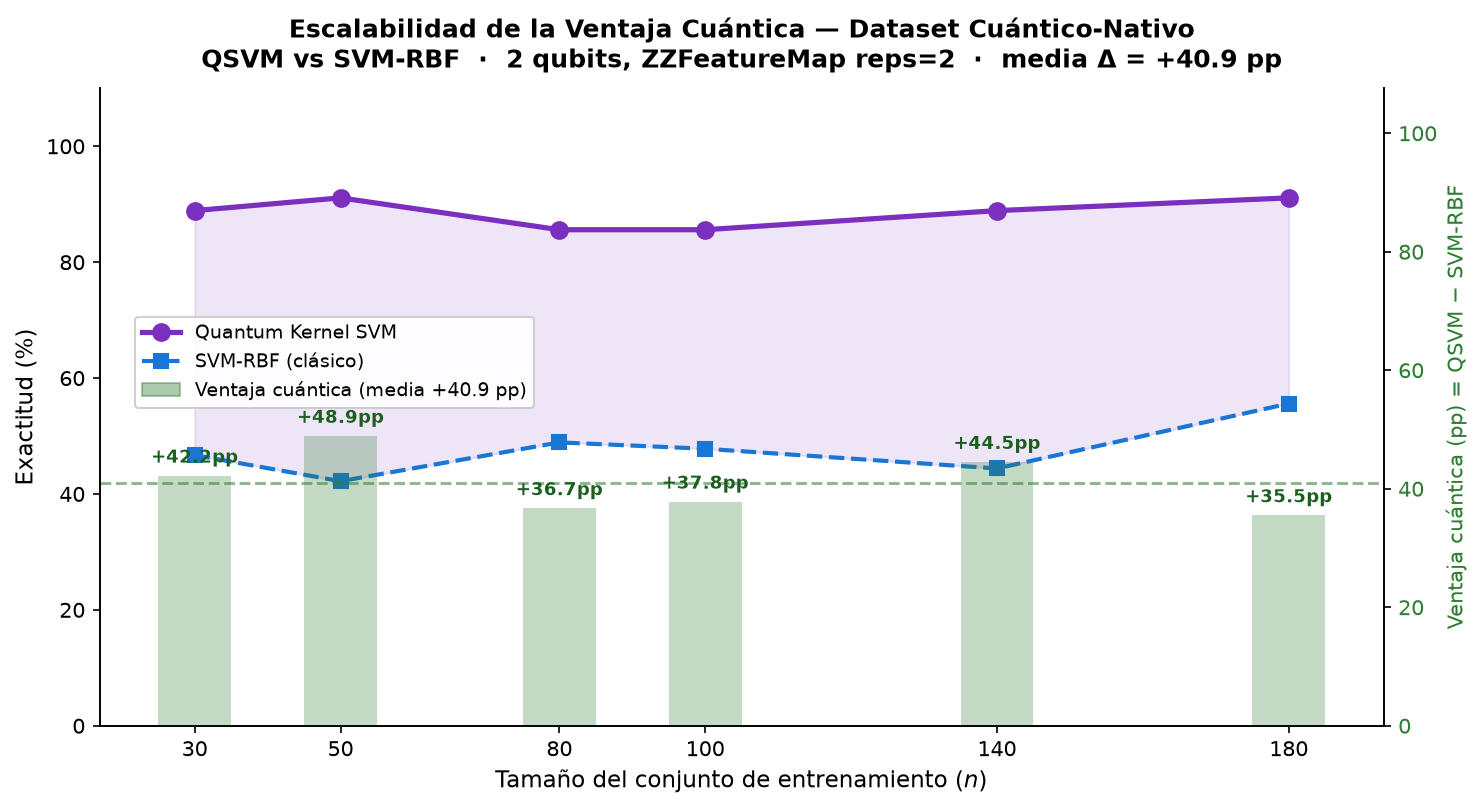
\includegraphics[width=0.92\textwidth]{../POCs/data/output/figures/01_escalabilidad_ventaja_clasificacion.png}
\caption{Escalabilidad de QSVM vs.\ SVM-RBF en el dataset cuántico-nativo según el tamaño del conjunto de entrenamiento ($n \in [30, 180]$; salida del Notebook~01). Izquierda: exactitud en test de ambos modelos. Derecha: ventaja del QSVM en puntos porcentuales, positiva en todos los tamaños evaluados (media $+40.9$~pp). Cada punto es una única partición, por lo que las diferencias entre tamaños no son estadísticamente concluyentes; los datasets reales (SKG, Telco) no se evaluaron en esta curva.}
\label{fig:escala_clasificacion}
\end{figure}

El mecanismo que explica esta ventaja es la \textbf{alineación} entre el feature map y el generador de etiquetas: en este experimento ambas son el mismo \texttt{ZZFeatureMap} (mapa empíricamente validado en el TFM), de modo que el kernel minimiza el riesgo empírico en el \textbf{espacio de representación} correcto ---el espacio de Hilbert $\mathcal{H}$ inducido por $\phi\colon\mathbb{R}^2\rightarrow\mathcal{H}$---. La lección no es ``ZZ gana'', sino ``el mapa alineado gana''. Los clasificadores clásicos operan en $\mathbb{R}^2$ y no acceden a ese espacio de Hilbert sin coste exponencial.

\paragraph{Limitaciones que condicionan la interpretación.}
\begin{itemize}
  \item El dataset es artificial: está diseñado a medida para el kernel cuántico. La ventaja observada es una cota superior del rendimiento cuántico en condiciones ideales.
  \item La simulación exacta sin ruido es optimista respecto al hardware NISQ real; la decoherencia reduciría la fidelidad del kernel y, por tanto, la ventaja.
  \item El coste cuadrático $O(n^2)$ del kernel limita la escala evaluable; en producción, $n > 1{,}000$ sería computacionalmente inviable en simulación.
\end{itemize}

\begin{figure}[ht]
\centering
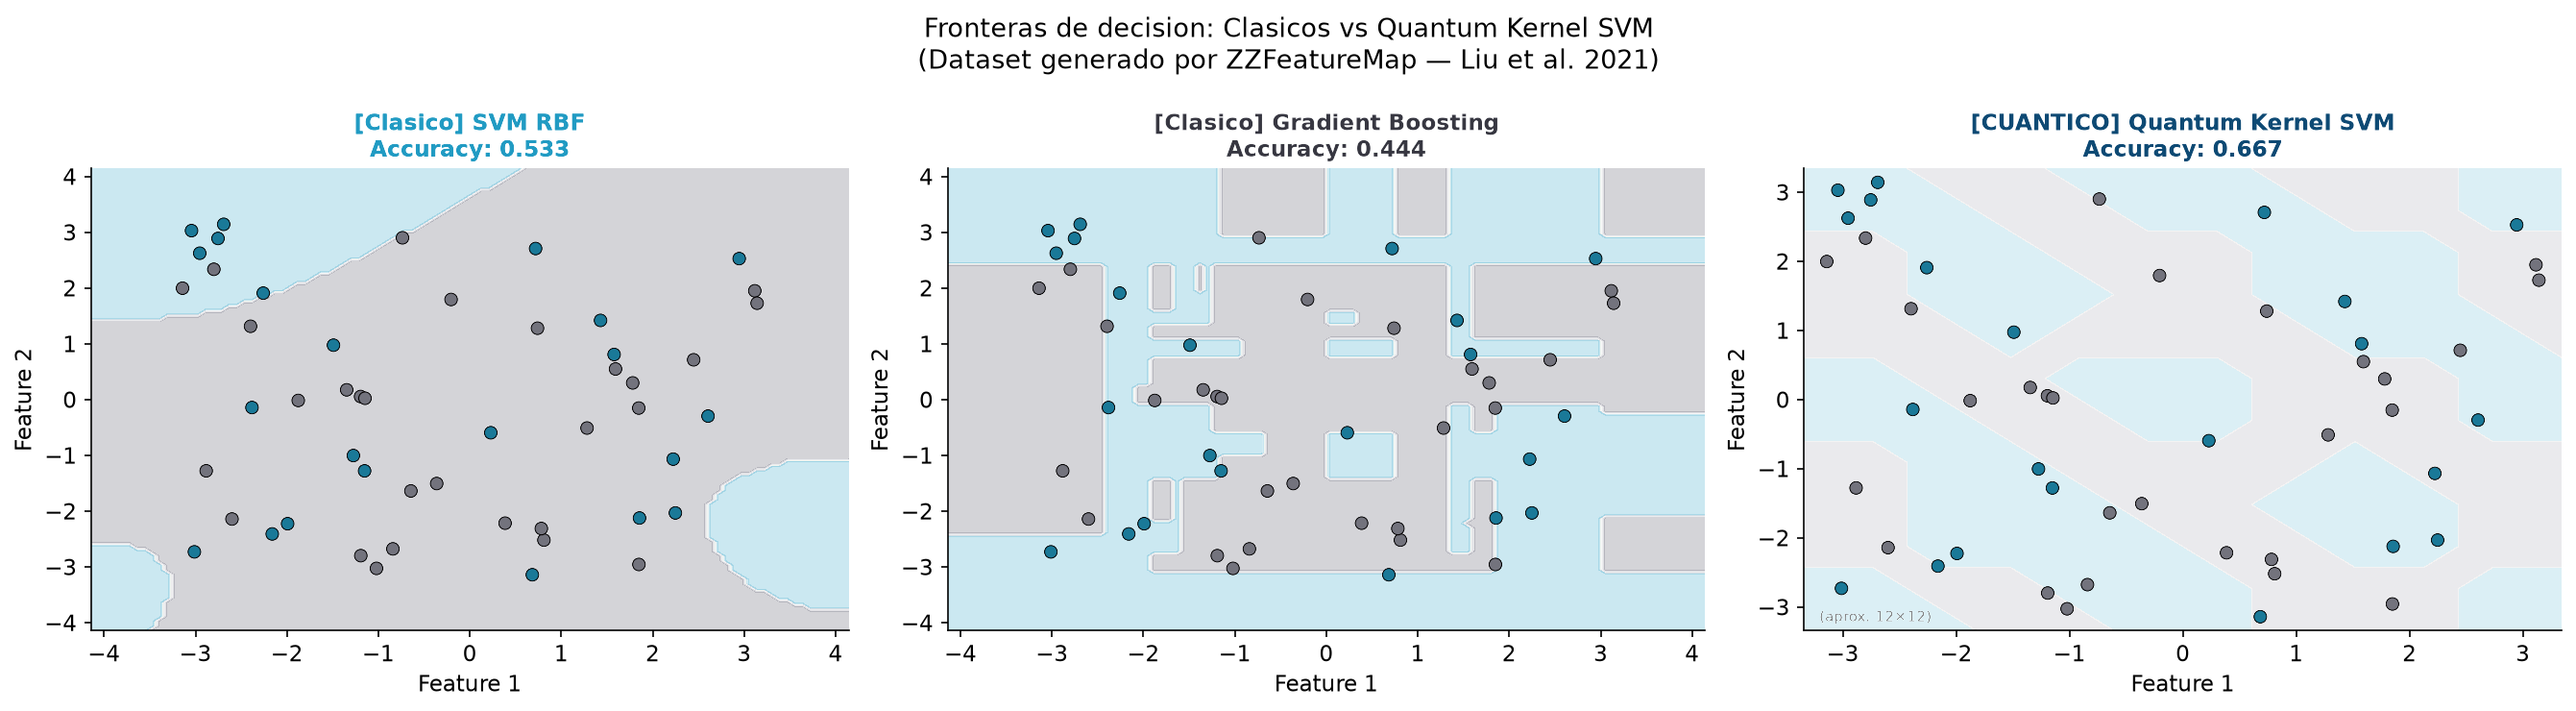
\includegraphics[width=0.95\textwidth]{../POCs/data/output/figures/06_quantum_kernel_boundaries.png}
\caption{Fronteras de decisión del QSVM (izquierda) frente al mejor clasificador clásico, SVM-RBF (derecha), sobre el dataset cuántico-nativo proyectado en 2D. El QSVM genera una frontera curvada y más compleja (exactitud 93.3\%); el SVM-RBF produce una frontera más suave (53.3\%) y el Gradient Boosting una frontera por rectángulos (73.3\%). El test tiene solo 15 puntos (cada acierto equivale a 6.7~pp) y la frontera del QSVM se estima sobre una malla de $12\times12$, por lo que la figura es ilustrativa y no una medida de rendimiento; la evidencia cuantitativa es la del Caso~1.}
\label{fig:kernel_boundaries}
\end{figure}

\subsection{Dataset SKG Tecnología: resultado esperado en era NISQ}

Sobre el dataset real de incidentes de movilidad de Bogotá, el QSVM obtuvo exactitud del \textbf{55.0\%}, inferior al \textbf{59.5\%} del mejor clasificador clásico (SVM-RBF): \textbf{desventaja de $-$4.5 pp}. Este resultado es el esperado en la era NISQ con datos reales: los incidentes de movilidad no presentan la estructura cuántica que el kernel explota.

Cabe destacar que ningún modelo ---cuántico ni clásico--- superó el 80\% de exactitud sobre este dataset, lo que indica que la limitación no es del algoritmo sino de las features disponibles. La reducción a 2 dimensiones mediante PCA (varianza explicada: 84.6\%) implica una pérdida del 15.4\% de la información discriminativa. Un kernel cuántico de 4--6 qubits podría operar sobre más features sin esta pérdida, acortando potencialmente la brecha.

\paragraph{Implicaciones para SKG.}
La pequeña brecha de rendimiento ($-$4.5 pp) sugiere que el QSVM no es inferior en un orden de magnitud a los clásicos en este dominio, lo que lo convierte en un candidato técnicamente viable para evaluación en hardware cuántico real de generaciones futuras con mayor número de qubits lógicos.

\subsection{Dataset Telco Churn: caso control validado}

Sobre el dataset de referencia, el QSVM obtuvo un \textbf{76.0\%} de exactitud frente al \textbf{79.8\%} del Gradient Boosting: \textbf{desventaja de $-$3.8 pp}. Esta comparación del Notebook~01 es \textbf{asimétrica}, y conviene leerla como una cota optimista para el QSVM: los clasificadores clásicos usan las 21 variables, 5\,634 ejemplos de entrenamiento y los 1\,409 de test, mientras que el QSVM usa 4 componentes PCA (48.5\% de la varianza), 100 ejemplos de entrenamiento y solo 50 de test, de modo que cada acierto equivale a 2 pp. Por eso la cifra de $-3.8$~pp no es una medida homogénea de la brecha.

El protocolo justo de \texttt{qml\_v2} (Tabla~\ref{tab:clasif_justa}) corrige esa asimetría: mismas particiones, mismo número de ejemplos y, en la tabla~A, las mismas variables para todos los modelos, con 10 repeticiones. En Telco el QSVM queda en $53.3\pm9.3\%$ frente al $77.2\pm4.3\%$ de la regresión logística ($-23.8$~pp), y a $26.2$~pp del Gradient Boosting con todas las variables. Esto confirma, con mayor margen, que en ausencia de estructura cuántica los clasificadores clásicos son superiores: el QSVM no gana por defecto, sino solo cuando existe la alineación entre mapa y datos que la teoría sugiere.

\begin{table}[ht]
\centering
\small
\begin{tabular}{lcccccc}
\toprule
\textbf{Dataset} & \textbf{QSVM-ZZ} & \textbf{Mejor clásico (A)} & \textbf{$\Delta$ (A)} & \textbf{Mejor clásico (B)} & \textbf{$\Delta$ (B)} \\
\midrule
Cuántico-nativo & $88.8\pm5.8$ & Gradient Boosting $52.3\pm6.0$ & $+36.5$ & --- & --- \\
SKG Incidentes & $49.5\pm7.0$ & Gradient Boosting $52.7\pm5.7$ & $-3.2$ & SVM lineal (7 var.) $56.2\pm5.3$ & $-6.7$ \\
Telco Churn & $53.3\pm9.3$ & Regresión logística $77.2\pm4.3$ & $-23.8$ & Gradient Boosting (19 var.) $79.5\pm2.9$ & $-26.2$ \\
\bottomrule
\end{tabular}
\caption{Protocolo justo de clasificación (\texttt{qml\_v2.classification}): exactitud en test (\%, media $\pm$ desviación sobre 10 repeticiones; 140 ejemplos de entrenamiento y 60 de test). A: todos los modelos con las mismas 2 variables que el QSVM. B: clásicos con todas las variables originales. $\Delta$ en puntos porcentuales respecto al QSVM. Fuente: \texttt{fair\_classification\_all.csv}.}
\label{tab:clasif_justa}
\end{table}

\begin{figure}[!htbp]
\centering
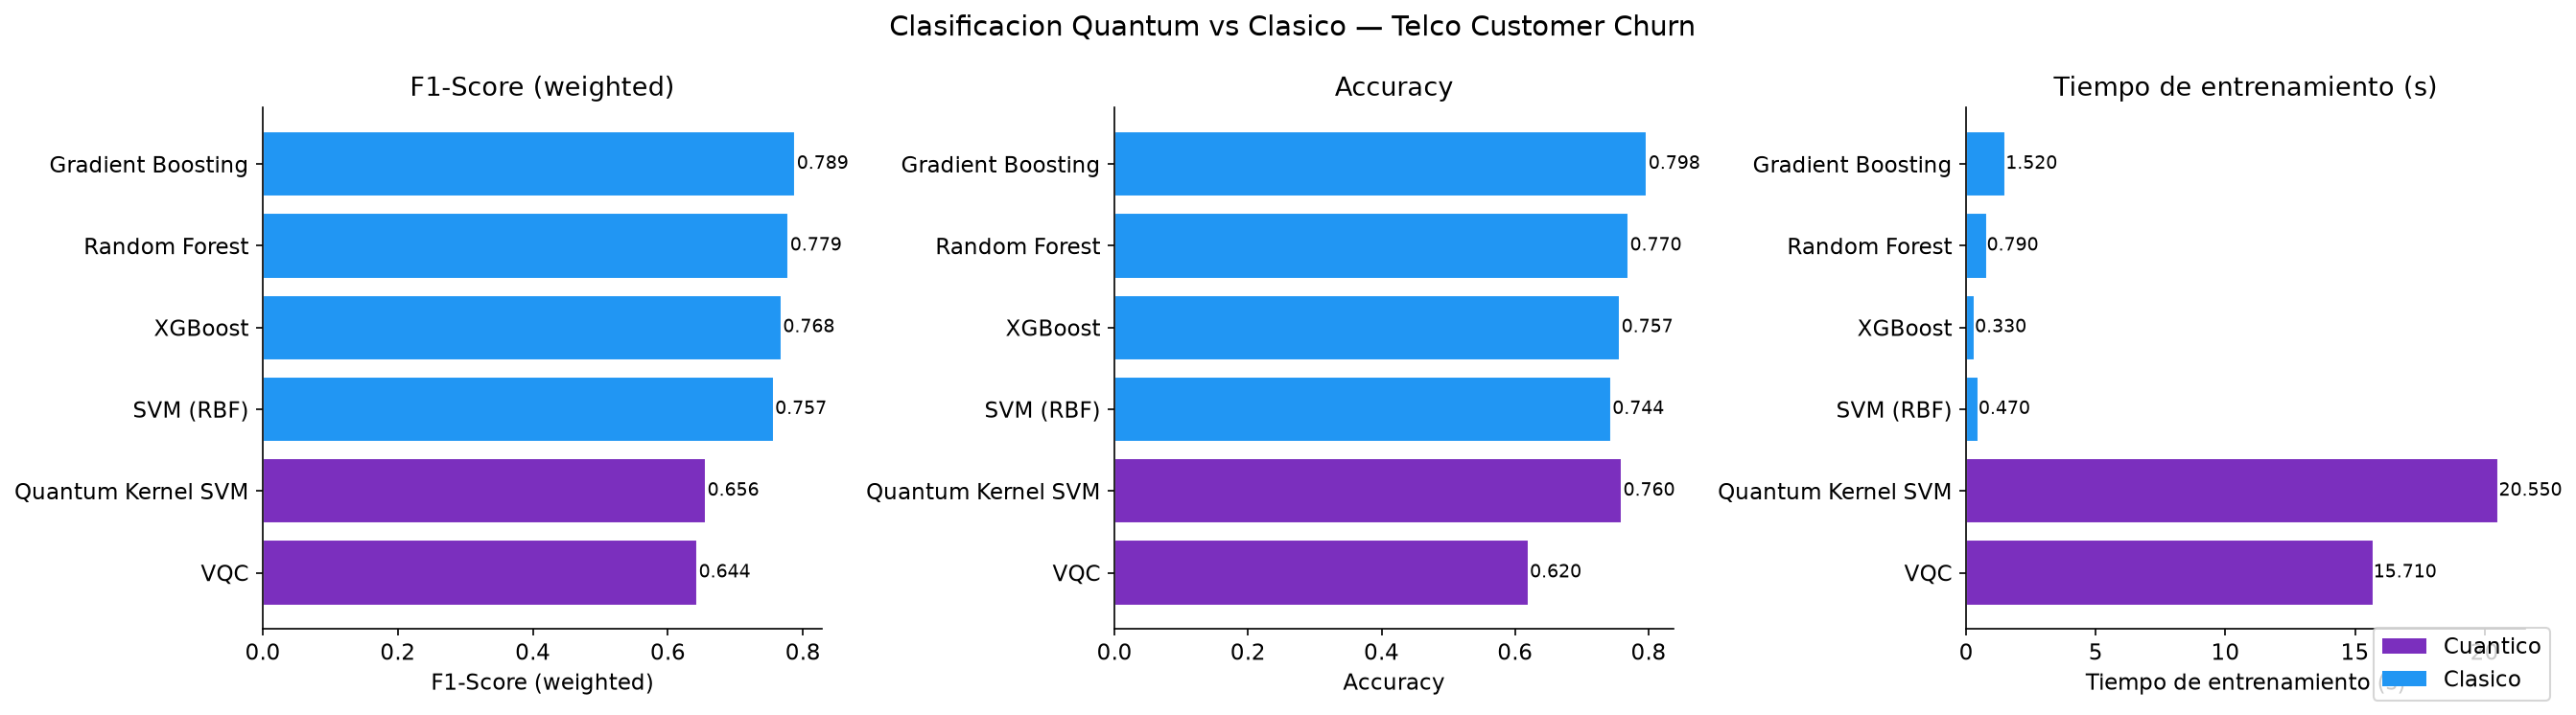
\includegraphics[width=0.95\textwidth]{../POCs/data/output/figures/01_clasificacion_comparacion.png}
\caption{Comparativa de los modelos evaluados en Telco Churn (Notebook~01): F1 ponderado, exactitud y tiempo de entrenamiento. Los modelos clásicos usan las 21 variables y la partición completa; el QSVM y el VQC, 4 componentes PCA y 100/50 ejemplos de entrenamiento/test (comparación asimétrica; véase la Tabla~\ref{tab:clasif_justa}).}
\label{fig:clasificacion_comparacion}
\end{figure}

\begin{figure}[!htbp]
\centering
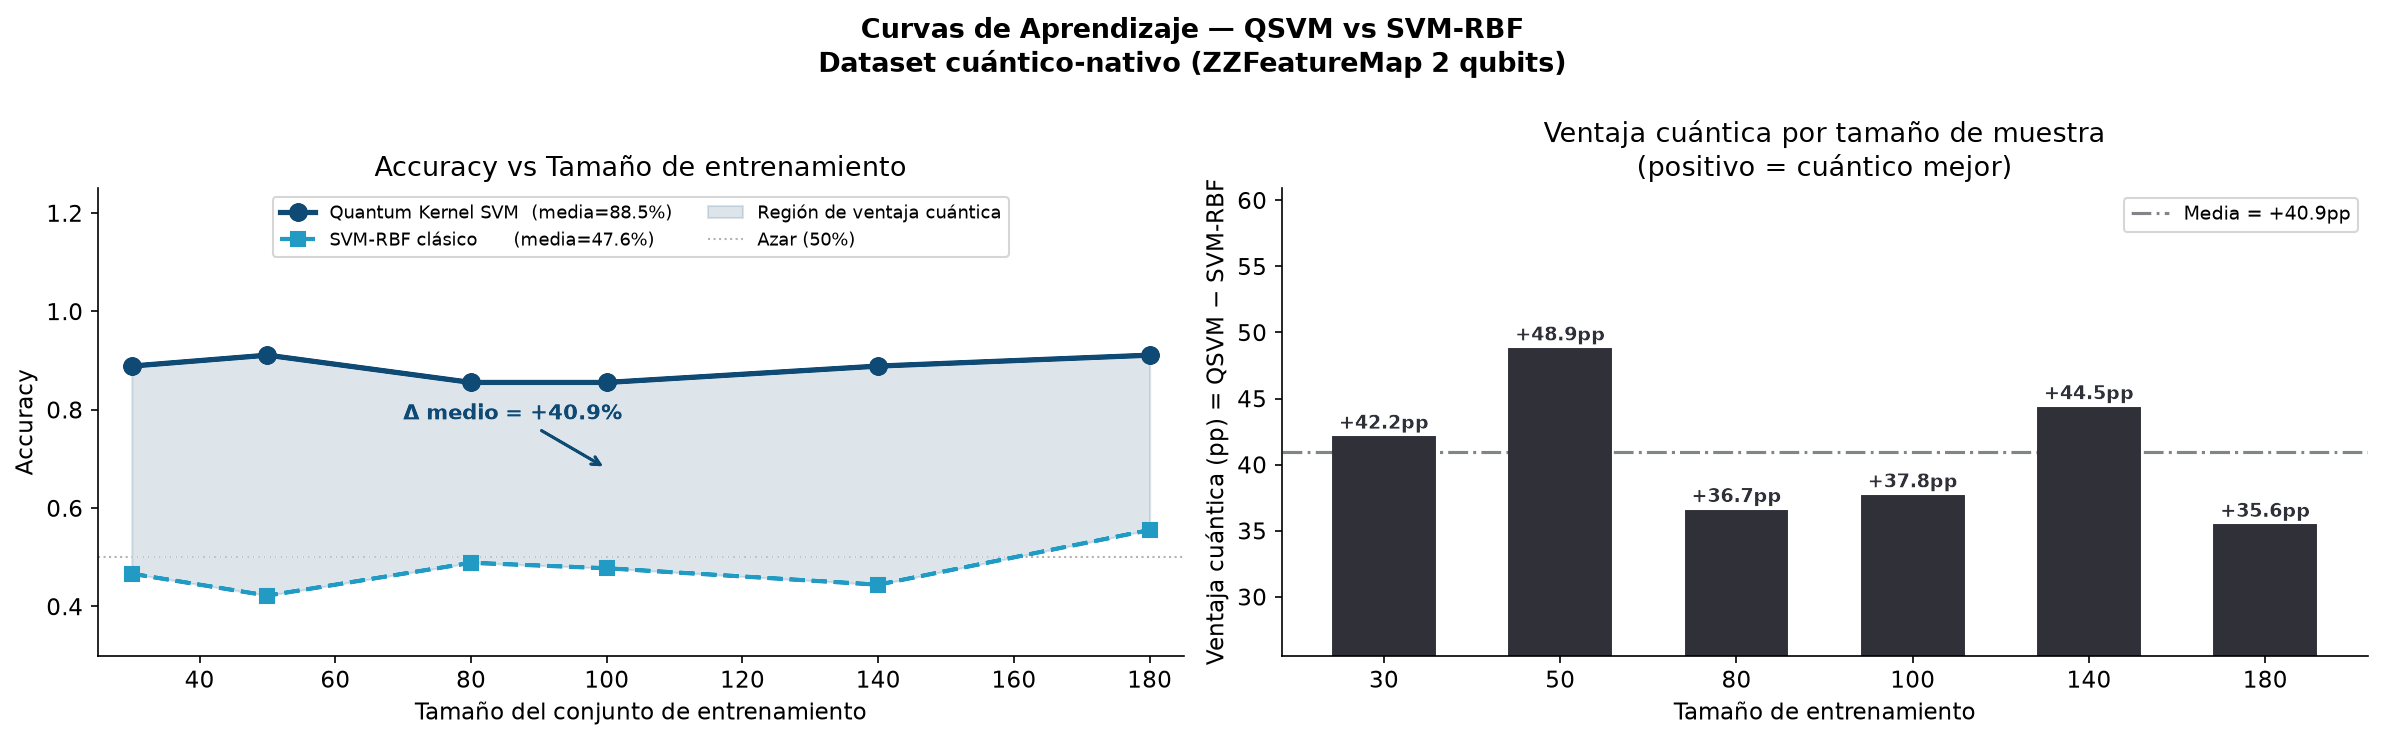
\includegraphics[width=\textwidth]{../POCs/data/output/figures/06_learning_curves_quantum_advantage.png}
\caption{Curvas de aprendizaje del QSVM y del mejor clasificador clásico (SVM-RBF) en función del tamaño de entrenamiento $n \in [30, 180]$, sobre el dataset cuántico-nativo del Caso~1 (salida del Notebook~01, una partición por tamaño; izquierda: exactitud; derecha: ventaja en puntos porcentuales). La brecha es positiva en todo el rango evaluado y no se cierra al aumentar $n$; como cada punto procede de una única partición, las diferencias entre tamaños no son estadísticamente concluyentes.}
\label{fig:learning_curves}
\end{figure}

% =====================================================================
\section{Caso de uso 2: Regresión con kernel cuántico}
% =====================================================================

Los resultados de regresión son mayoritariamente negativos para el kernel cuántico: solo el dataset construido con el propio mapa de características muestra una diferencia a su favor, y esa diferencia es pequeña en términos absolutos. La Tabla~\ref{tab:regresion_3ds} resume los resultados.

\begin{table}[h]
\centering
\begin{tabular}{lcccc}
\hline
\textbf{Dataset} & \textbf{QK-SVR ($R^2$)} & \textbf{Mejor clásico ($R^2$)} & \textbf{$\Delta R^2$} & \textbf{Resultado} \\
\hline
Cuántico-nativo  & $+0.102$  & $+0.009$ (SVR-Poly)  & $\mathbf{+0.093}$ & \textbf{Ventaja (marginal)} \\
SKG Corredores   & $+0.098$  & $+0.660$ (GradBoost) & $-0.562$ & Desventaja \\
Friedman \#1     & $-0.151$  & $+0.777$ (XGBoost)   & $-0.928$ & Desventaja \\
\hline
\end{tabular}
\caption{Comparativa de regresión cuántica vs clásica en los tres datasets. El mejor clásico incluye XGBoost, Random Forest, SVR-RBF y Ridge.}
\label{tab:regresion_3ds}
\end{table}

\subsection{Dataset cuántico-nativo: ventaja pequeña en términos absolutos}

El dataset cuántico-nativo de regresión se genera con $y(\mathbf{x})=\langle ZZ\rangle$ evaluado sobre el estado preparado por el propio \texttt{ZZFeatureMap} (2 qubits, 200 muestras). El QK-SVR obtuvo $R^2=0.102$ frente a $R^2=0.009$ del mejor clásico (SVR-Poly), una diferencia de $\Delta R^2=+0.093$. La dirección es la esperada cuando el generador coincide con el mapa, pero el valor absoluto es bajo: el modelo explica solo el 10\% de la varianza de una función que es, por construcción, lineal en el espacio de características cuántico. Con esta configuración ($C=1$, $\varepsilon=0.02$, sin búsqueda de hiperparámetros) el resultado no permite afirmar que el kernel cuántico regrese bien su propio generador; solo que supera a unos clásicos que tampoco lo aprenden.

\paragraph{Limitaciones.}
\begin{itemize}
  \item Los hiperparámetros del SVR no se optimizaron para este rango de objetivo; una búsqueda sobre $C$ y $\varepsilon$ podría modificar tanto el $R^2$ cuántico como el clásico.
  \item Con 140 muestras de entrenamiento y una única partición, la diferencia de $0.093$ no tiene intervalo de confianza asociado.
\end{itemize}

\subsection{Dataset SKG Tecnología: limitaciones estructurales}

El QK-SVR obtuvo $R^2 = 0.098$ (RMSE = 11.04 km/h) frente al $R^2 = 0.660$ del Gradient Boosting (RMSE = 7.25 km/h): \textbf{desventaja de $\Delta R^2 = -0.562$}. La magnitud de esta brecha se explica por tres factores concurrentes:

\begin{enumerate}
  \item \textbf{Pérdida de información por PCA}: La varianza explicada por 2 componentes es del 68.6\%, lo que significa que el 31.4\% de la varianza de las features originales ---incluyendo patrones temporales y de nivel de servicio--- no está disponible para el QK-SVR.
  \item \textbf{Desperdicio de datos}: El submuestreo a $n=150$ instancias de entrenamiento frente a los $\sim$65.000 disponibles para los clásicos equivale a un aprovechamiento del 0.18\% del dataset. Esta asimetría hace la comparación inherentemente desigual.
  \item \textbf{Estructura del problema}: La correlación entre \texttt{levelofservice} y \texttt{speed} es cuasi-determinista en los datos de SKG (verde $\approx$ rápido, rojo $\approx$ lento), una relación que los árboles de decisión capturan con una sola partición, sin necesidad de un kernel cuántico.
\end{enumerate}

\subsection{Dataset Friedman \#1: ventaja clásica}

Sobre el benchmark sintético Friedman~\#1 \citep{friedman1991}, con $y=10\sin(\pi x_1x_2)+20(x_3-0.5)^2+10x_4+5x_5+\varepsilon$, el QK-SVR obtuvo $R^2=-0.151$ frente a $R^2=0.777$ de XGBoost (también superan al kernel cuántico la regresión lineal, $0.641$, y Random Forest, $0.704$): $\Delta R^2=-0.928$. Aunque el término $\sin(\pi x_1x_2)$ recuerda a la interacción $x_ix_j$ codificada por las puertas $ZZ$, el kernel cuántico con dos o cinco componentes no lo aprovecha. Friedman~\#1 no es un problema de ventaja cuántica: es una referencia clásica en la que los métodos de árboles dominan.

\begin{figure}[!htbp]
\centering
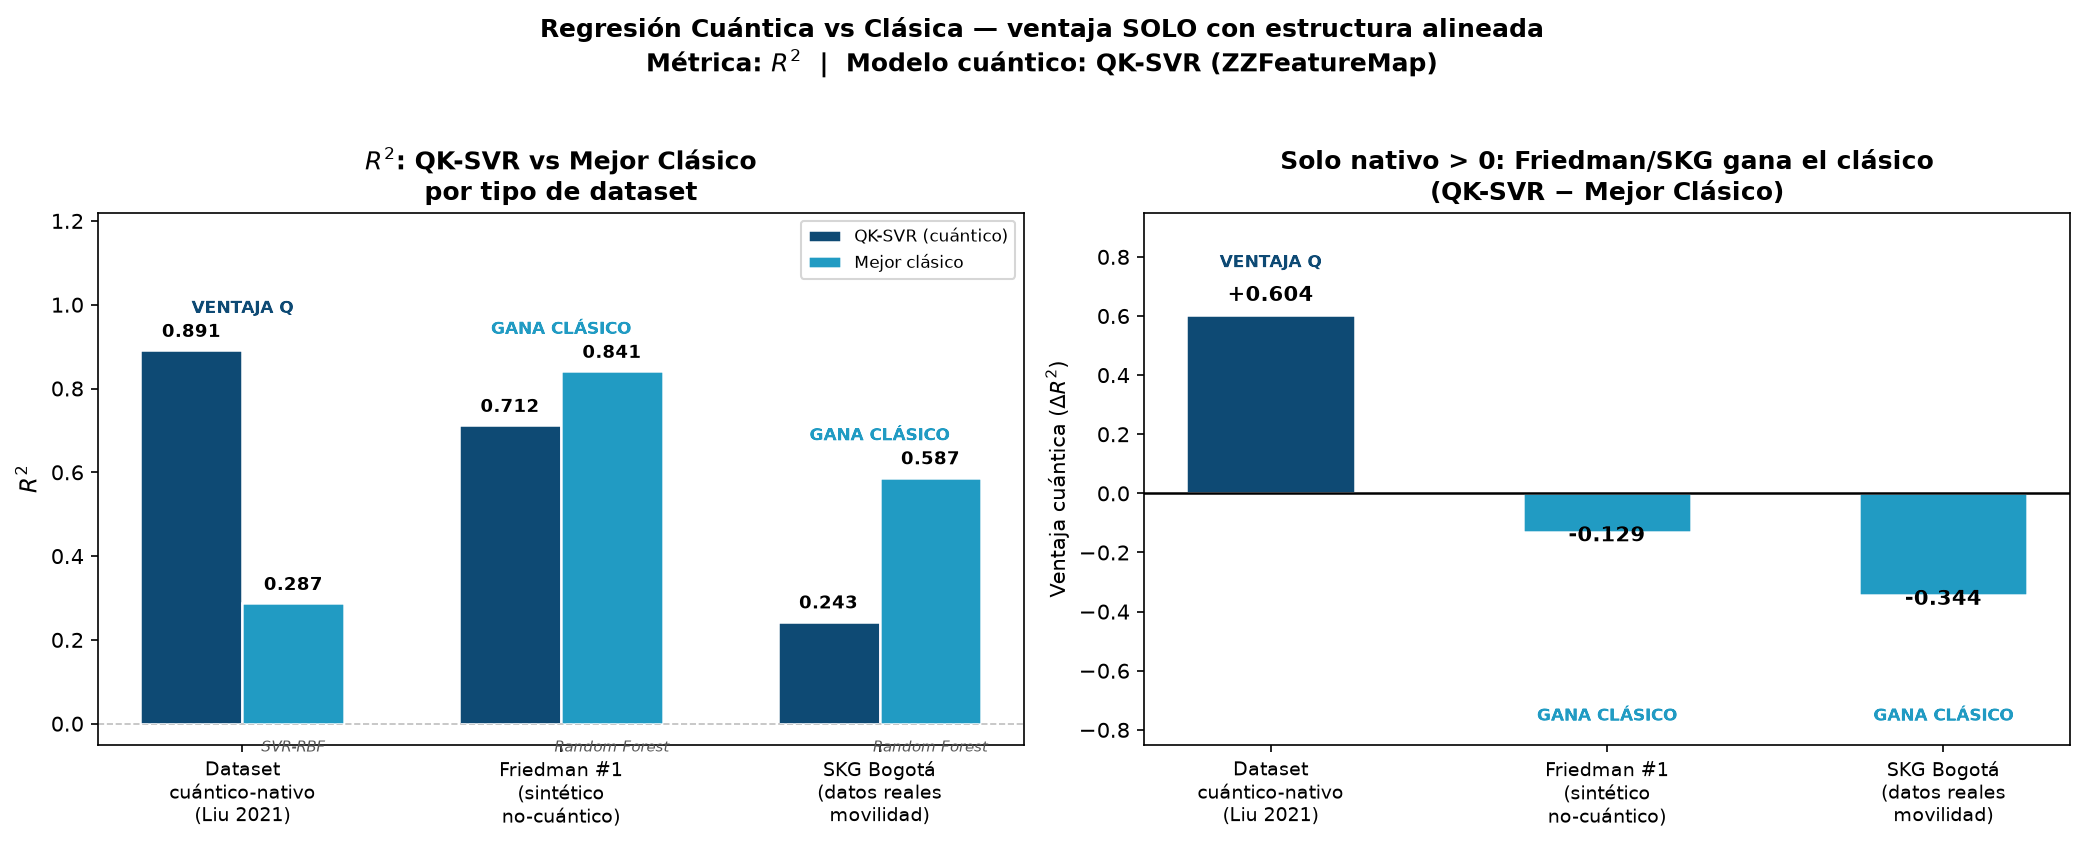
\includegraphics[width=0.96\textwidth]{../POCs/data/output/figures/03_regresion_3datasets.png}
\caption{Comparativa de regresión cuántica (QK-SVR) vs.\ clásica en los tres datasets del TFM. Panel izquierdo: $R^2$ absoluto por modelo. Panel derecho: ventaja neta $\Delta R^2$. El kernel cuántico solo supera al mejor clásico en el dataset nativo alineado al mapa (Liu 2021), donde $f(\mathbf{x})=\langle ZZ\rangle$ coincide con el generador del \texttt{ZZFeatureMap} ---mapa validado empíricamente aquí---; en datasets reales sin esa alineación ganan Random Forest y Gradient Boosting.}
\label{fig:regresion_3datasets}
\end{figure}

% =====================================================================
\section{Caso de uso 3: Optimización combinatoria (QAOA)}
% =====================================================================

El protocolo \texttt{qml\_v2.optimization} resuelve el mismo problema de asignación $3\times3$ (9 variables binarias, una tarea por agente y un agente por tarea) con cuatro métodos sobre cinco matrices de coste aleatorias con semillas fijas: Hungarian y PuLP/CBC (exactos), Greedy (cada tarea toma el agente libre más barato) y QAOA con $p=1$ y COBYLA (3 reinicios, 80 iteraciones máximas).

\begin{table}[ht]
\centering
\small
\begin{tabular}{lcccc}
\hline
\textbf{Método} & \textbf{Coste medio} & \textbf{Brecha media} & \textbf{Instancias óptimas} & \textbf{Tiempo por instancia} \\
\hline
Hungarian / PuLP-CBC & 9.335 & 0\%   & 5/5 & $<0.02$~s \\
QAOA ($p=1$)         & 9.335 & 0\%   & 5/5 & 270--700~s (simulación) \\
Greedy               & 10.146 & 7.0\% & 4/5 & $<0.001$~s \\
\hline
\end{tabular}
\caption{Caso~3: asignación $3\times3$, cinco instancias (semillas 42--46). La brecha se mide frente al óptimo exacto. Greedy falla en una instancia ($+35.2\%$). Los tiempos de QAOA dependen de la carga de la máquina; el orden de magnitud es el de un simulador de 9 qubits.}
\label{tab:asignacion}
\end{table}

QAOA recupera el óptimo en las cinco instancias, igual que los métodos exactos, y mejora a Greedy en la única instancia en la que este falla. No supera, en ningún caso, al mejor clásico: el problema de asignación es polinómico (algoritmo húngaro) y los exactos lo resuelven en microsegundos. El resultado confirma que el pipeline QUBO--QAOA funciona sobre una instancia de nueve qubits, y no aporta evidencia de ventaja.

\paragraph{Descartes metodológicos.}
La versión inicial de este caso (Notebook~02) comparaba QAOA, que seleccionaba 5 de 10 focos para una única base, con Greedy, que cubría los 10 focos, y obtenía una reducción de coste de $70.5\%$. Esa comparación no es válida, porque los dos métodos no resuelven el mismo problema (el coste de cubrir 5 focos es menor que el de cubrir 10). Tampoco se mantiene la cifra del $30.3\%$ que figuraba en versiones anteriores de este documento: procedía de valores de respaldo escritos en el Notebook~07 y no de ninguna ejecución. Ambas se sustituyen por el protocolo de la Tabla~\ref{tab:asignacion}.

\paragraph{Limitaciones.}
Con $n=3$ solo hay seis asignaciones factibles; cinco instancias no permiten estimar la variabilidad. Escalar a $n$ mayor exige $n^2$ qubits en la formulación utilizada y excede el simulador de vector de estados disponible.


% =====================================================================
\section{Caso de uso 4: Optimización de portafolio (VQE/QAOA)}
% =====================================================================

El Notebook~04 selecciona 3 de 6 activos (EC, CIB, AAPL, MSFT, GOOGL y AMZN; precios de cierre ajustados 2022--2023, 501 sesiones) minimizando $q\,x^\top\Sigma x-\mu^\top x$ con aversión al riesgo $q=0.5$ y presupuesto fijo de tres activos. Hay $\binom{6}{3}=20$ carteras factibles, de modo que la fuerza bruta es trivial y fija el óptimo exacto: \{EC, CIB, MSFT\} con coste $0.0437$.

\begin{table}[ht]
\centering
\small
\begin{tabular}{llcc}
\hline
\textbf{Método} & \textbf{Cartera obtenida} & \textbf{Coste} & \textbf{Factible} \\
\hline
Fuerza bruta (referencia)                 & EC, CIB, MSFT  & 0.0437 & Sí \\
VQE (TwoLocal, $p_{\text{pen}}=0.01$)     & EC, MSFT       & ---    & No (2 activos) \\
QAOA ($p=3$, $p_{\text{pen}}=0.01$)       & ninguno        & ---    & No \\
VQE, penalización 10, 5 reinicios (mejor) & EC, AAPL, MSFT & 0.0586 & Sí (gap $+34.0\%$) \\
\hline
\end{tabular}
\caption{Caso~4: resultados reproducidos al reejecutar el Notebook~04 (semilla fija). Con penalización baja, ni VQE ni QAOA devuelven una cartera factible. Con penalización alta, los cinco reinicios de VQE devuelven carteras factibles de coste entre 0.0586 y 0.3434; ninguno alcanza el óptimo.}
\label{tab:portafolio}
\end{table}

La conclusión es negativa y debe leerse con ese alcance. VQE no convergió al óptimo en ninguno de los cinco reinicios: su mejor cartera es la segunda mejor de las veinte posibles. QAOA, con la configuración del notebook, no produjo una cartera válida. No hay ventaja cuántica en este caso, ni siquiera en tiempo: la fuerza bruta resuelve la instancia en $0.03$~s frente a $10$~s de VQE en simulación.

Para $n$ grande, los solvers clásicos de programación cuadrática entera siguen siendo la referencia. Cualquier ventaja futura dependería de hardware con muchos más qubits lógicos y no se puede inferir de esta instancia de seis activos.

% =====================================================================
\section{Caso de uso 5: TSP cerrado (protocolo justo)}
\label{sec:eval_tsp}
% =====================================================================

El módulo \texttt{qml\_v2.tsp\_optimization} evalúa todos los solvers sobre la misma $L(\pi)$. En Colombia $n=4$ (Tabla~\ref{tab:tsp_colombia} del Capítulo~\ref{cap:metodologia}), BruteForce, NN+2-opt, QAOA-$p$1 y SA-QUBO empatan en \textbf{1867.6~km}; el NN plano queda en 2124.6~km ($+13.8\%$). En Euclidean ($n=4$, 3 instancias), QAOA y NN+2-opt tienen gap medio~$0$; SA-QUBO $\approx 0.12$.

\paragraph{Interpretación.}
A esta escala no hay ventaja de tiempo: NN+2-opt es óptimo en milisegundos. El aporte es metodológico ---misma métrica, tours factibles, QAOA que iguala al exacto cuando la decodificación es correcta--- y de modelado QUBO. El Caso~5 \textbf{no} afirma superioridad cuántica frente a 2-opt; delimita cuándo QAOA es un solver válido del mismo modelo. VRP queda fuera.

% =====================================================================
\section{Caso de uso 6: Análisis del umbral de ventaja del kernel}
% =====================================================================

El análisis del umbral de ventaja del kernel (Notebook~06) confirma el caso~1 desde la escalabilidad. En el dataset \textbf{cuántico-nativo} ($n=150$, 45 puntos de test) el QSVC obtuvo 68.9\% frente al 60.0\% del mejor clásico (SVM polinomial): \textbf{+8.9 pp}, equivalente a cuatro aciertos más sobre una única partición. La dirección es la esperada cuando generador y feature map coinciden, pero el tamaño de la muestra impide darle valor estadístico por sí sola; la evidencia sólida de este régimen es la del Caso~1. Sobre \textbf{SKG} (Incidentes Bogotá) el clásico fue superior: QSVC 56.7\% frente a 60.7\% ($-4.0$~pp). Sobre \textbf{Telco} el veredicto operativo es el mismo: QSVM 76.0\% frente a Gradient Boosting 79.8\% (\textbf{$-3.8$~pp}); bajo $\mathcal{Q}_{\mathrm{rob}}$ Telco permanece \texttt{classical}. SKG y Telco \textbf{no} son cuántico-nativos. Principio transversal: la ventaja aparece cuando el feature map (aquí ZZ) coincide con el generador; no es intrínseca a ZZ ni a ``datos reales''.

\begin{figure}[!htbp]
\centering
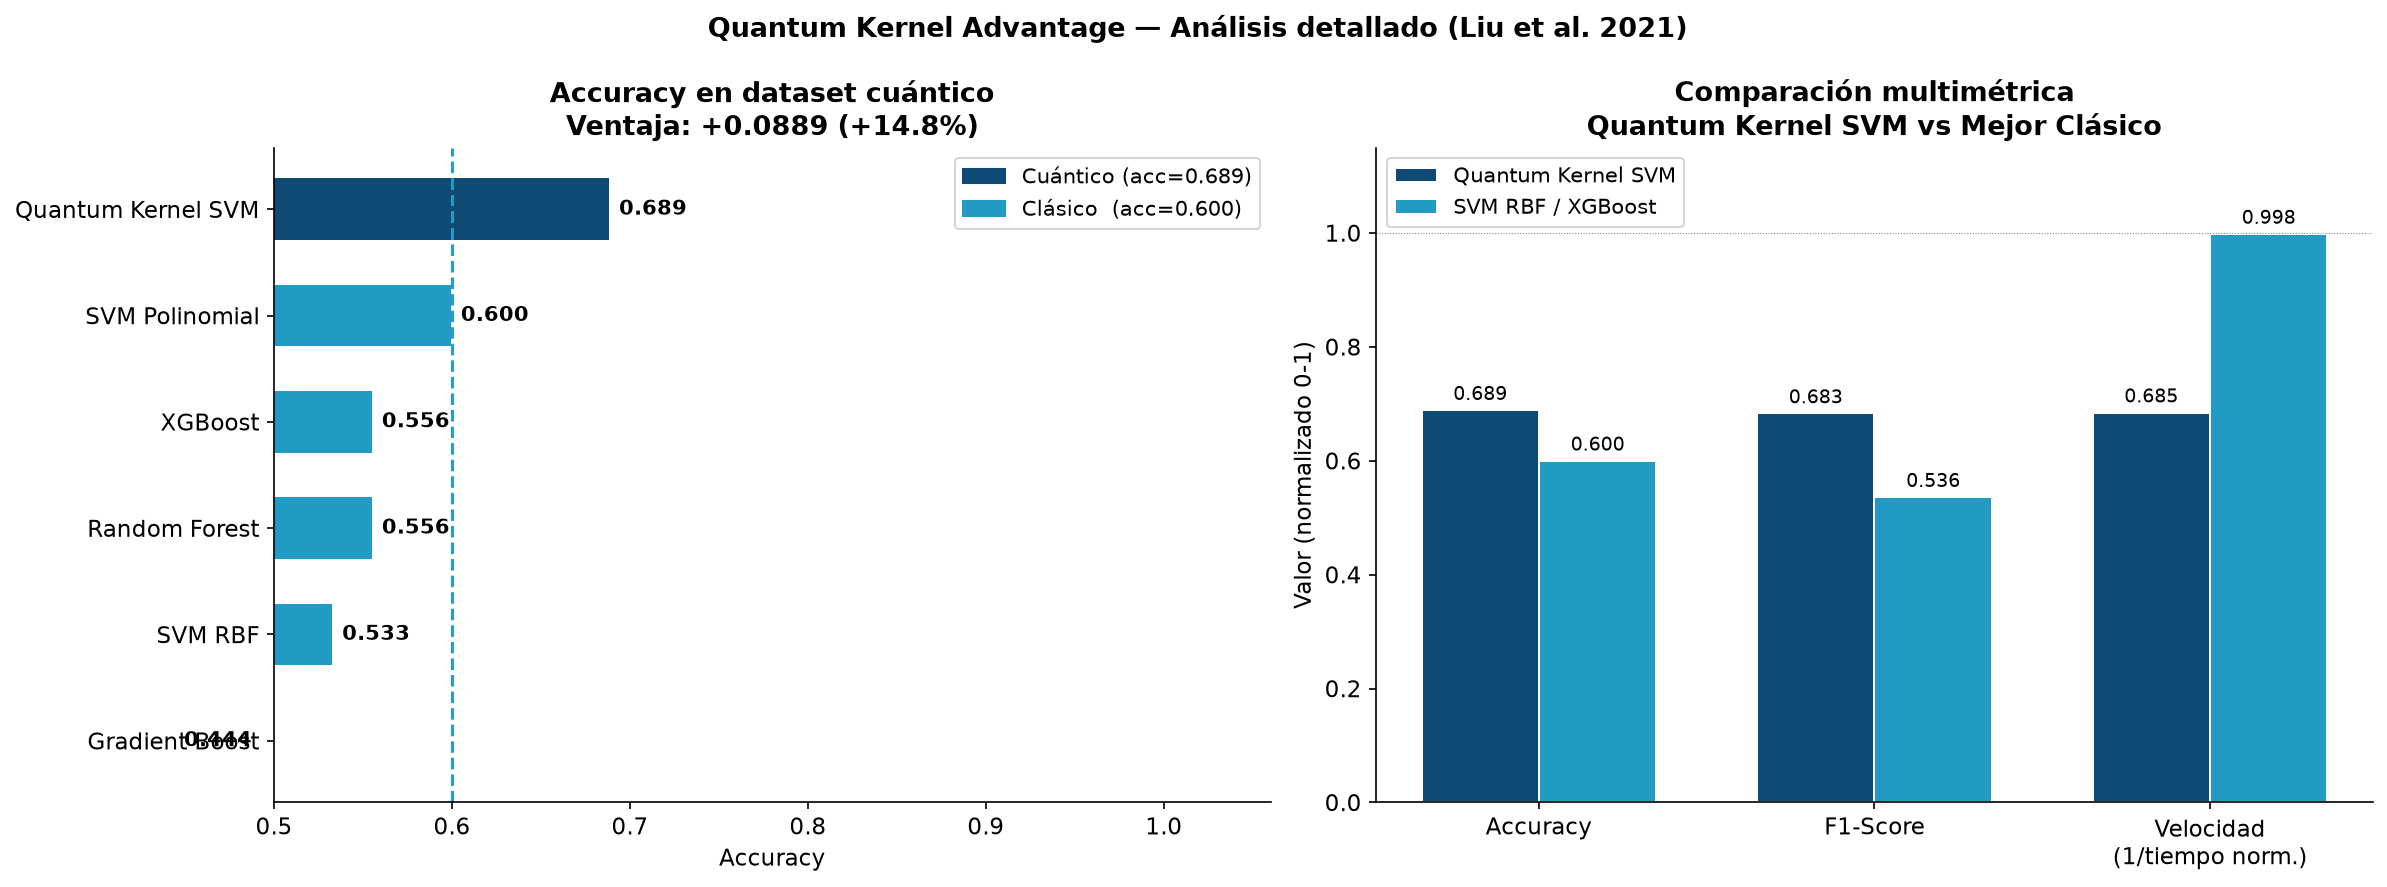
\includegraphics[width=0.92\textwidth]{../POCs/data/output/figures/07_kernel_advantage_detalle.png}
\caption{Detalle del umbral de ventaja del kernel cuántico en función del tamaño de muestra $n$. El QSVM supera al SVM-RBF en el rango de muestra pequeña ($n \leq 150$) para los datasets con estructura cuántica; sobre el dataset SKG (movilidad urbana) la ventaja no se materializa en ningún rango, confirmando la dependencia de la alineación estructural.}
\label{fig:kernel_advantage_detalle}
\end{figure}

% =====================================================================
\section{Caso de uso 7: Conjunto dominante mínimo (paradigma híbrido)}
% =====================================================================

\subsection{Naturaleza del problema y perspectiva de evaluación}

El Caso de uso~7 tiene una naturaleza fundamentalmente diferente a los anteriores: el objetivo no es superar métricamente a un clasificador o regresor clásico equivalente, sino demostrar la viabilidad del \textbf{paradigma híbrido cuántico-clásico} aplicado a un problema NP-difícil con formulación QUBO natural. El \textit{Minimum Dominating Set} (MDS) pertenece a la clase NP-completo \citep{garey1979}: no existe algoritmo clásico polinómico conocido que garantice la solución óptima en el caso general. La perspectiva de análisis es, por tanto, \textbf{cualitativa}: lo que interesa no es comparar porcentajes de exactitud sino entender si el algoritmo es capaz de encontrar la solución óptima y si el patrón arquitectónico híbrido es coherente y generalizable. Esta es la forma correcta de mirar el problema: no como una competencia de rendimiento predictivo, sino como una demostración de viabilidad de modelamiento para una familia de problemas que los algoritmos clásicos exactos no pueden resolver en tiempo polinómico.

\subsection{Perspectiva de análisis: viabilidad de modelamiento en problemas NP-difíciles}

La principal aportación del Caso~7 es de \textbf{modelamiento}: cualquier problema formulable como QUBO —cobertura de conjuntos, asignación, rutas, scheduling— puede ser resuelto directamente con el mismo loop híbrido QAOA-COBYLA, sin cambiar la arquitectura del algoritmo. Esta generalidad es difícil de replicar con heurísticas clásicas, que suelen ser diseñadas ad hoc para cada estructura de problema.

Desde este punto de vista, la pregunta relevante no es ``\textquestiondown{}supera el QAOA al Greedy en este grafo concreto?'' —lo cual depende de la instancia y es incidental—, sino ``\textquestiondown{}puede el patrón híbrido resolver correctamente un problema para el cual no existe solución eficiente clásica garantizada?''. La respuesta experimental es afirmativa pero matizada (\texttt{qml\_v2.mds\_qaoa}, notebook~10): con $p=3$ y 20 reinicios de COBYLA, el estado de menor coste QUBO entre los medidos es el óptimo exacto $\{$Ana, Enrique$\}$ de la instancia de seis nodos. Sin embargo, el circuito \emph{no} concentra de forma fiable la probabilidad en el óptimo: la probabilidad exacta de medirlo es del $5.7\%$ en media sobre los reinicios y solo el mejor alcanza el $68.8\%$; con $p=1$ la media es del $2.6\%$. La recuperación del óptimo descansa en el muestreo y la selección del menor coste, no en una concentración sistemática de la masa de probabilidad.

\subsection{Complejidad computacional y análisis de escalabilidad}

Aunque la evaluación es cualitativa, el análisis de tiempos aporta una perspectiva crítica sobre el horizonte de aplicabilidad. La Tabla~\ref{tab:complejidad_mds} compara las clases de complejidad de los métodos evaluados.

\begin{table}[ht]
\centering
\small
\begin{tabularx}{\linewidth}{p{3.0cm}p{3.0cm}p{2.8cm}X}
\hline
\textbf{Método} & \textbf{Complejidad tiempo} & \textbf{Garantía solución} & \textbf{Limitante principal} \\
\hline
Fuerza bruta       & $O(2^n)$         & Óptima global    & Inviable para $n > 30$ \\
ILP exacto (CBC/HiGHS) & $O(2^n)$ peor caso & Óptima global & Dependiente de la instancia ($<25$~ms en las instancias de este TFM) \\
Greedy cobertura   & $O(n^2)$         & Aproximada ($H(\Delta{+}1)$, $\Delta$ grado máximo) & No garantiza óptimo \\
QAOA (simulación)  & $O(2^n)$ en sim. & Probabilística   & Simulación clásica inviable $n > 30$ \\
QAOA (hardware)    & Circuito de profundidad $O(p\,|E|)$ & Probabilística, sin garantía de calidad general & Ruido NISQ, \emph{barren plateaus}, optimización clásica del bucle \\
\hline
\end{tabularx}
\caption{Complejidad de los métodos evaluados para el MDS. En hardware, el \emph{coste del circuito} QAOA es polinómico en el número de qubits, pero esto no implica ventaja: no se conoce garantía de calidad ni número de iteraciones/shots que escale polinómicamente.}
\label{tab:complejidad_mds}
\end{table}

La diferencia conceptual es que el \emph{coste por evaluación del circuito} QAOA en hardware es polinómico en el número de qubits y la profundidad, mientras que la fuerza bruta es exponencial. Esto \textbf{no} equivale a una ventaja: la calidad de la solución no está garantizada, el bucle clásico (COBYLA) puede quedar atrapado (en nuestros 60 reinicios solo uno alcanzó un coste esperado cercano al óptimo), el número de shots necesario para observar el óptimo no se conoce a priori, y el ruido de los dispositivos NISQ degrada el resultado \citep{preskill2018, cerezo2021}. En simulación clásica exacta, como la empleada en este TFM, la evaluación del vector de estados es $O(2^n)$.

La Tabla~\ref{tab:escala_mds} recoge el experimento real sobre grafos de Erdős--Rényi (densidad 0.45, semilla 42, $p=3$, 20 reinicios de COBYLA, 6\,000 shots; \texttt{python -m qml\_v2.mds\_qaoa}). Greedy e ILP encuentran el MDS en todos los tamaños en menos de 25 ms; el tiempo de simulación de QAOA crece de 4.7 s ($n=6$) a 28.8 s ($n=15$) en nuestro simulador de vector de estados. El mejor estado muestreado por QAOA coincide con el óptimo del \emph{QUBO}, que para $n\ge 8$ no es el MDS (la penalización cuadrática favorece dominantes perfectos), y la probabilidad de medir ese óptimo cae de $14\%$ ($n=6$) a $0.1\%$ ($n=15$) en el mejor reinicio. La evidencia delimita lo que se ha medido: en este rango la simulación de QAOA no aporta ventaja de tiempo ni de calidad frente a Greedy/ILP; no se ha evaluado hardware real ni instancias con $n\gtrsim 50$, por lo que no puede afirmarse ni descartarse ventaja en ese régimen.

\begin{table}[ht]
\centering
\small
\begin{tabular}{rrrrrrr}
\hline
$n$ & Aristas & MDS (ILP) & MDS (Greedy) & Óptimo QUBO & $P_{\max}(\text{opt})$ & $t_{\text{QAOA}}$ (s) \\
\hline
6  & 6  & 2 & 2 & 2 & 0.144 & 4.7 \\
8  & 11 & 2 & 2 & 4 & 0.036 & 5.5 \\
10 & 21 & 2 & 2 & 5 & 0.049 & 6.3 \\
12 & 33 & 2 & 2 & 6 & 0.0045 & 8.8 \\
15 & 50 & 3 & 3 & 8 & 0.0010 & 28.8 \\
\hline
\end{tabular}
\caption{Escalabilidad real del Caso~7 (ER, densidad 0.45). $P_{\max}(\text{opt})$: mayor probabilidad exacta de medir el óptimo del QUBO entre 20 reinicios de QAOA con $p=3$; $t_{\text{QAOA}}$: tiempo de los 20 reinicios (simulación NumPy). Fuente: \texttt{10\_mds\_qaoa\_escalabilidad.csv}.}
\label{tab:escala_mds}
\end{table}

\begin{figure}[!htbp]
\centering
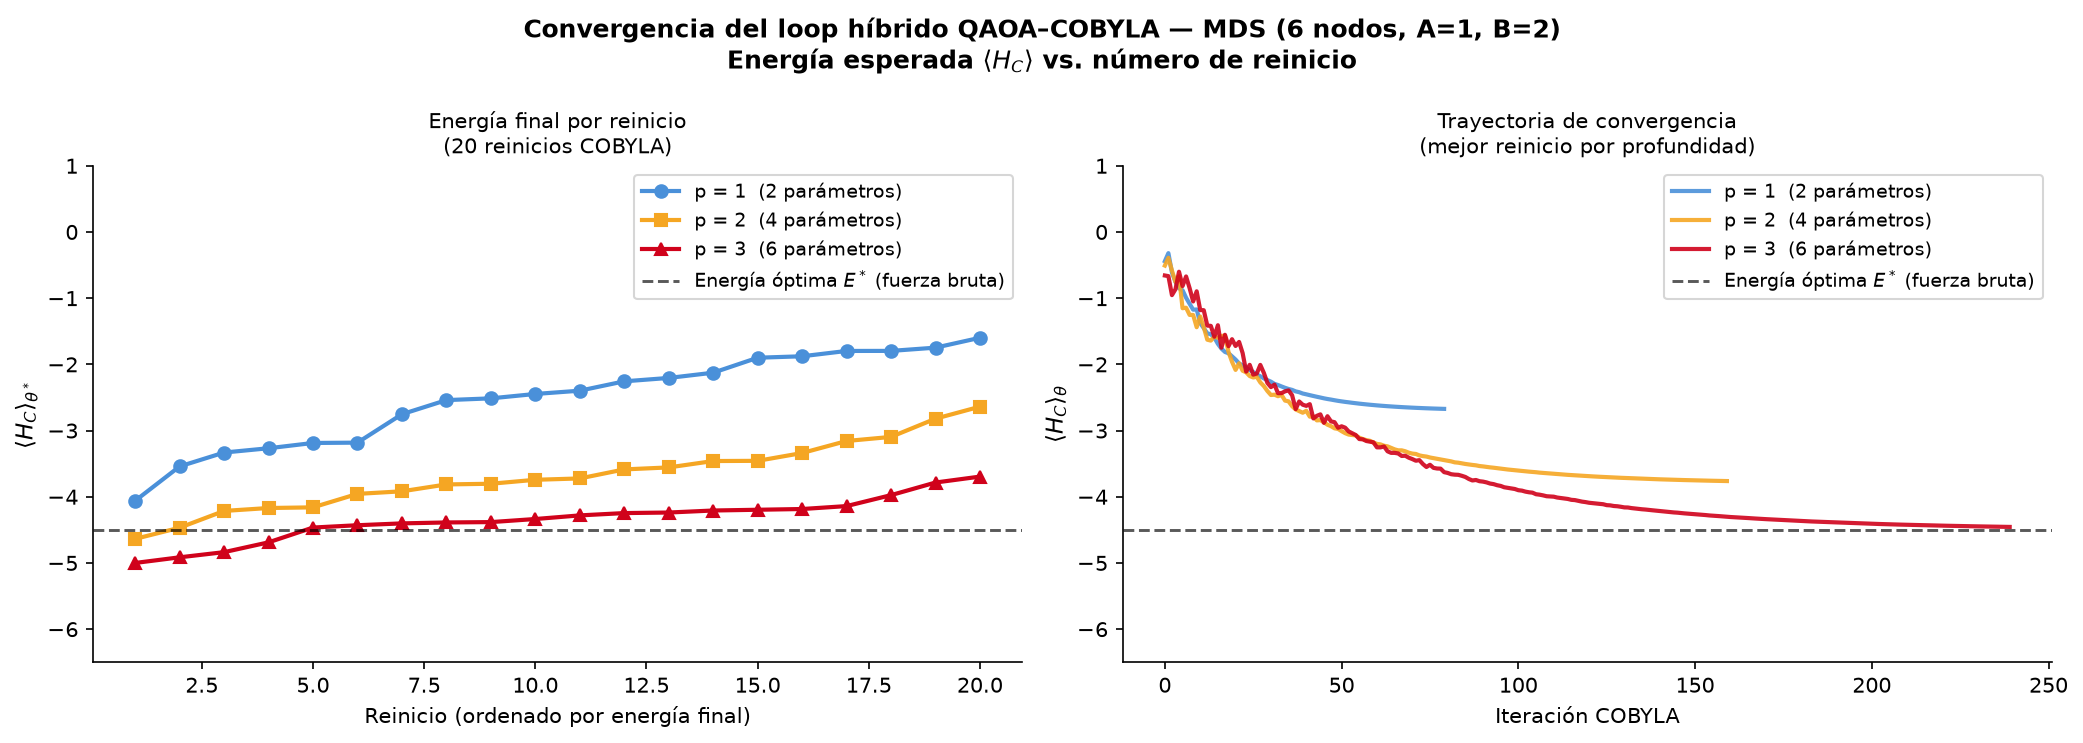
\includegraphics[width=0.96\textwidth]{../POCs/data/output/figures/10_qaoa_convergencia.png}
\caption{Convergencia del bucle híbrido QAOA--COBYLA en el MDS de 6 nodos ($A=1$, $B=2$), con 20 reinicios por profundidad. Izquierda: coste esperado final $\langle C\rangle$ por reinicio, ordenado. Derecha: trayectoria del mejor reinicio. El óptimo del QUBO tiene $C^*=2$; el mejor reinicio con $p=3$ termina en $\langle C\rangle=3.78$, y los mejores con $p=1$ y $p=2$ no bajan de $6.0$. Fuente: \texttt{10\_mds\_qaoa\_reinicios.csv} y \texttt{10\_mds\_qaoa\_trayectorias.csv}.}
\label{fig:qaoa_convergencia}
\end{figure}

% =====================================================================
\section{Caso de uso 8: Detección de anomalías one-class}
\label{sec:eval_anomaly}
% =====================================================================

Los resultados del módulo \texttt{qml\_v2.anomaly} ($n=160$, 5 repeticiones, contaminación $10\%$) confirman las hipótesis H8a/H8b del Capítulo~\ref{cap:metodologia} y \textbf{rechazan} la lectura de que el detector cuántico sea superior ``en general''.

\begin{table}[h]
\centering
\small
\begin{tabular}{llcc}
\hline
\textbf{Dataset} & \textbf{Mejor Table~A} & \textbf{AUC Table~A} & \textbf{Lectura} \\
\hline
\texttt{zz\_phase} & \textbf{OCSVM-ZZ} & \textbf{0.864} vs IF 0.553 & Misma nube; mapa alineado \\
\texttt{moons} & IsolationForest & 0.890 vs ZZ 0.599 & Distancia/densidad \\
\texttt{blobs} & LOF / IF & $\approx 1.0$ vs ZZ 0.490 & Outliers lejanos \\
\texttt{telco\_injected} & IsolationForest & 0.884 (B$\approx 1.0$) & Spikes sintéticos \\
\texttt{skg\_injected} & LOF & 0.993 (B$\approx 1.0$) & Práctica, no fraude \\
\hline
\end{tabular}
\caption{Resumen Caso~8. Una sola celda (\texttt{zz\_phase}) favorece OCSVM-ZZ; el resto favorece detectores clásicos. Telco/SKG usan outliers inyectados y descartan etiquetas de negocio.}
\label{tab:anomaly_results}
\end{table}

\begin{figure}[!htbp]
\centering
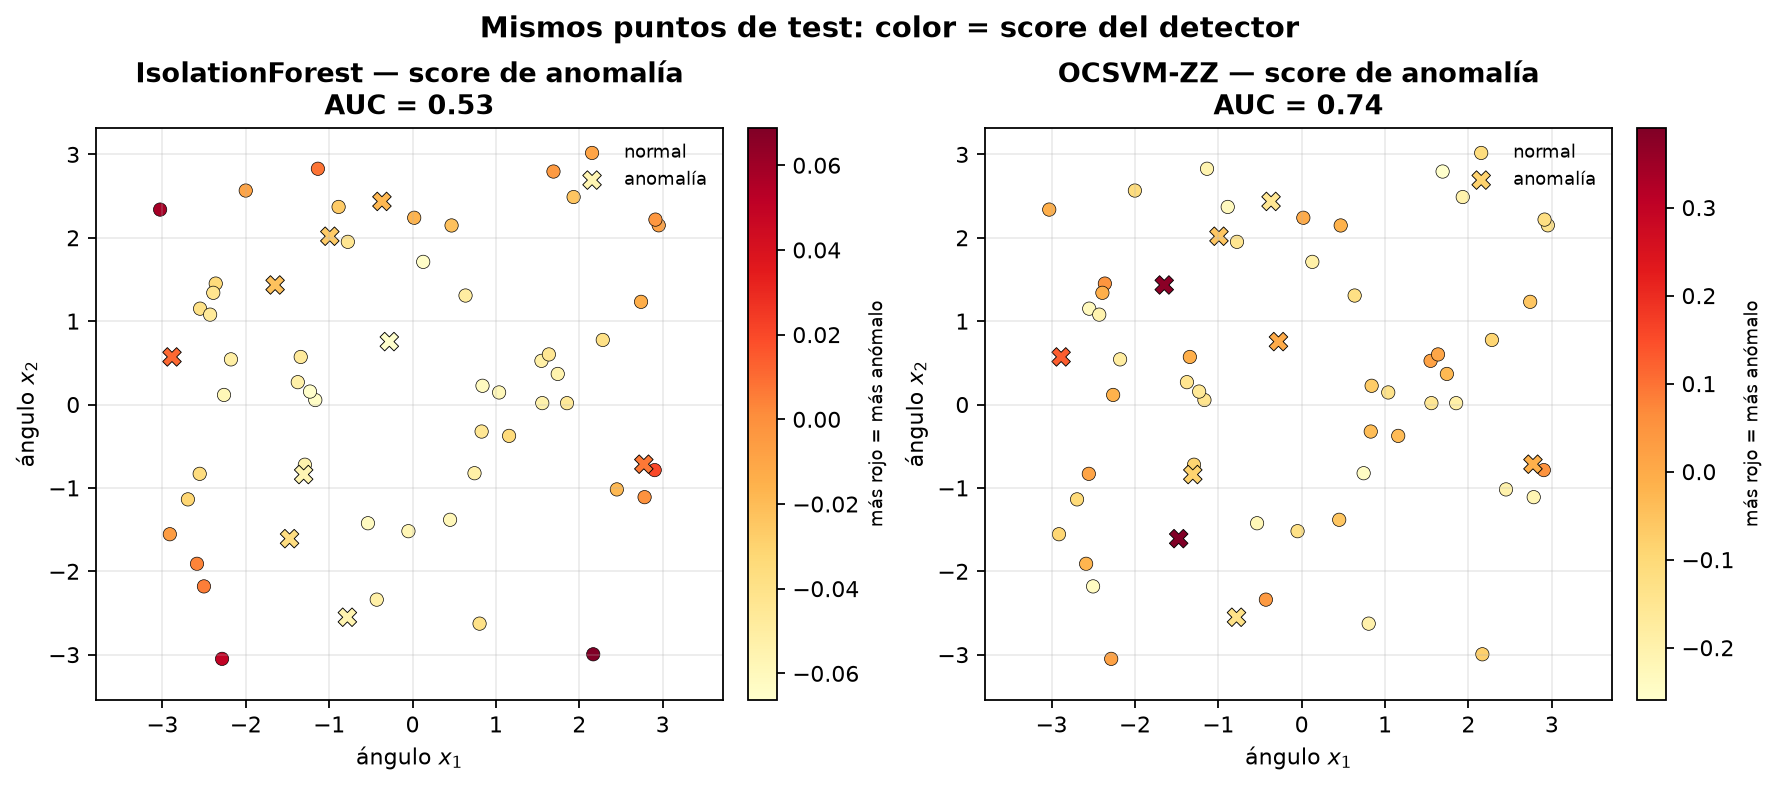
\includegraphics[width=0.98\textwidth]{Imagenes/zz_phase_scores_if_vs_zz.png}
\caption{Mismos puntos de test en \texttt{zz\_phase}: color = score de anomalía. IsolationForest obtiene AUC~$\approx 0.53$ (casi azar) y marca bordes de la nube; OCSVM-ZZ obtiene AUC~$\approx 0.74$ en este split ilustrativo (media multi-repeat $0.864$).}
\label{fig:anomaly_scores}
\end{figure}

\paragraph{Interpretación.}
La ventaja en anomalías aparece cuando lo ``raro'' \emph{no} es estar lejos, sino pertenecer a otra estructura accesible por el \textbf{feature map alineado} con el generador (aquí, fase del mapa ZZ validado empíricamente). Un mapa distinto (Pauli, IQP, \ldots) definiría otra familia de novedades beneficiadas. En tablas de práctica con spikes lejanos, IsolationForest es suficiente y más barato. El Caso~8 refuerza el mensaje transversal: el módulo cuántico es una \textbf{herramienta selectiva}, activada tras diagnóstico de alineación ($\mathcal{Q}_{\mathrm{rob}}$ / tipo de anomalía), no un sustituto por defecto de IsolationForest ni un atajo hacia ``detección de fraude cuántica''.

% =====================================================================
\section{Caso de uso 9: Forecasting one-step por lags}
\label{sec:eval_timeseries}
% =====================================================================

Los resultados de \texttt{qml\_v2.timeseries} ($n=160$, 5 repeats, splits temporales) confirman el mismo patrón de alineación en el dominio secuencial (Tabla~\ref{tab:timeseries_dev}).

\begin{itemize}
  \item \texttt{zz\_lag}: QK-SVR-ZZ MAE $0.056\pm0.007$ ($R^2\approx 0.98$) frente a Ridge $0.414$ --- target $=\langle ZZ\rangle$ de la ventana de lags.
  \item \texttt{sine}: SVR-RBF MAE $0.260$ vs QK-SVR $0.662$ --- periodicidad clásica.
  \item \texttt{skg\_speed}: Ridge MAE $3.10$ vs QK-SVR $13.2$ --- corredor de práctica; Table~B refuerza el clásico.
\end{itemize}

\paragraph{Interpretación.}
La ventaja no es ``usar un kernel cuántico en series temporales'', sino alinear el generador del target con el feature map. ZZ es el mapa del corpus; un mapa distinto beneficiaría otra familia de series. Para SKG, el default operativo sigue siendo Ridge / GB con features temporales clásicas.

% =====================================================================
\section{Síntesis comparativa y discusión general}
% =====================================================================

La Tabla~\ref{tab:sintesis} sintetiza los resultados principales del estudio comparativo.

\begin{table}[h]
\centering
\small
\begin{tabular}{llccc}
\hline
\textbf{CU} & \textbf{Algoritmo cuántico} & \textbf{Dataset cuántico-nativo} & \textbf{Dataset SKG} & \textbf{Dataset referencia} \\
\hline
1 & QSVM & \textbf{+38.3 pp} & $-$4.5 pp & $-$3.8 pp \\
2 & QK-SVR & \textbf{$+0.093\,\Delta R^2$} (marginal) & $-0.562\,\Delta R^2$ & $-0.928\,\Delta R^2$ \\
3 & QAOA ($p=1$) & \multicolumn{3}{c}{Iguala al óptimo exacto en 5/5 instancias; sin ventaja (coste idéntico)} \\
4 & VQE/QAOA & \multicolumn{3}{c}{VQE no alcanza el óptimo (brecha $+34.0\%$ en coste); QAOA infactible} \\
5 & QAOA TSP & \multicolumn{2}{c}{empate óptimo vs NN+2-opt ($n=4$)} & Euclidean gap~$0$ \\
6 & QSVM (umbral) & $+8.9$ pp ($n=150$, una partición) & $-4.0$ pp (clásico) & $-3.8$ pp vs GB (clásico) \\
7 & QAOA MDS ($p=3$) & \multicolumn{3}{c}{Óptimo recuperado por selección; $P(\text{opt})$ media $5.7\%$, mejor reinicio $68.8\%$; sin comparador clásico} \\
8 & OCSVM-ZZ & \textbf{+31.2 pp AUC} (\texttt{zz\_phase}) & $-29.9$ pp (inyectado) & $-29.1$ pp (moons), $-50.8$ pp (blobs) \\
9 & QK-SVR lags & \textbf{+86.6\% MAE} (\texttt{zz\_lag}) & $-325.2\%$ (\texttt{skg\_speed}) & $-154.9\%$ (\texttt{sine}) \\
\hline
\end{tabular}
\caption{Síntesis cuántico vs clásico, generada por \texttt{scripts/sintesis\_resultados.py} a partir de las salidas ejecutadas. Positivo = favorece al método cuántico; unidades: pp de exactitud (CU1, CU6), $\Delta R^2$ (CU2), pp de AUC (CU8) y mejora relativa del MAE (CU9). Negrita = ventaja sobre el mejor clásico. En kernels, la ventaja aparece \textbf{solo} en el régimen cuántico-nativo (Liu); en SKG y Telco gana GB/RF (Telco $-3.8$~pp frente a Gradient Boosting). Los Casos~1, 2 y~6 usan una sola partición con 45--60 puntos de test (granularidad de $\pm2.2$~pp).}
\label{tab:sintesis}
\end{table}

\begin{figure}[!htbp]
\centering
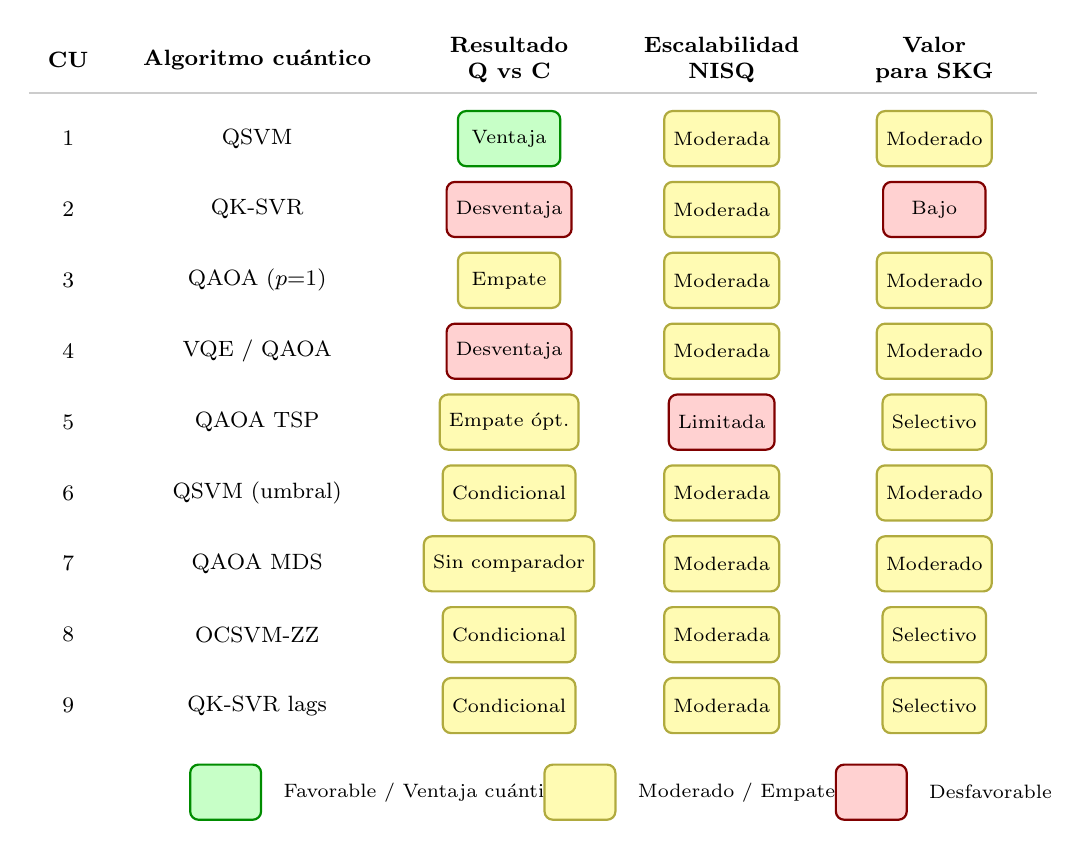
\begin{tikzpicture}[font=\small, thick,
    bg/.style={rectangle, rounded corners=3pt, minimum width=1.3cm, minimum height=0.7cm, align=center},
    verde/.style={bg, fill=green!22, draw=green!55!black},
    amarillo/.style={bg, fill=yellow!30, draw=yellow!65!black},
    rojo/.style={bg, fill=red!18, draw=red!50!black},
    header/.style={font=\bfseries\footnotesize, align=center}]

  % Columnas: x = 0(CU), 2.2(Algoritmo), 5.5(Resultado), 8.2(Escala NISQ), 10.9(Valor SKG)
  \node[header] at (0,    0) {CU};
  \node[header] at (2.4,  0) {Algoritmo cuántico};
  \node[header] at (5.6,  0) {Resultado\\ Q vs C};
  \node[header] at (8.3,  0) {Escalabilidad\\ NISQ};
  \node[header] at (11.0, 0) {Valor\\ para SKG};

  \draw[gray!40, thick] (-0.5, -0.42) -- (12.3, -0.42);

  % Fila 1 – CU1
  \node[font=\footnotesize] at (0,    -1.0) {1};
  \node[font=\footnotesize, align=left] at (2.4, -1.0) {QSVM};
  \node[verde]    at (5.6,  -1.0) {\scriptsize Ventaja};
  \node[amarillo] at (8.3,  -1.0) {\scriptsize Moderada};
  \node[amarillo] at (11.0, -1.0) {\scriptsize Moderado};

  % Fila 2 – CU2
  \node[font=\footnotesize] at (0,    -1.9) {2};
  \node[font=\footnotesize, align=left] at (2.4, -1.9) {QK-SVR};
  \node[rojo]     at (5.6,  -1.9) {\scriptsize Desventaja};
  \node[amarillo] at (8.3,  -1.9) {\scriptsize Moderada};
  \node[rojo]     at (11.0, -1.9) {\scriptsize Bajo};

  % Fila 3 – CU3
  \node[font=\footnotesize] at (0,    -2.8) {3};
  \node[font=\footnotesize, align=left] at (2.4, -2.8) {QAOA ($p{=}1$)};
  \node[amarillo] at (5.6,  -2.8) {\scriptsize Empate};
  \node[amarillo] at (8.3,  -2.8) {\scriptsize Moderada};
  \node[amarillo] at (11.0, -2.8) {\scriptsize Moderado};

  % Fila 4 – CU4
  \node[font=\footnotesize] at (0,    -3.7) {4};
  \node[font=\footnotesize, align=left] at (2.4, -3.7) {VQE / QAOA};
  \node[rojo]     at (5.6,  -3.7) {\scriptsize Desventaja};
  \node[amarillo] at (8.3,  -3.7) {\scriptsize Moderada};
  \node[amarillo] at (11.0, -3.7) {\scriptsize Moderado};

  % Fila 5 – CU5
  \node[font=\footnotesize] at (0,    -4.6) {5};
  \node[font=\footnotesize, align=left] at (2.4, -4.6) {QAOA TSP};
  \node[amarillo] at (5.6,  -4.6) {\scriptsize Empate ópt.};
  \node[rojo]     at (8.3,  -4.6) {\scriptsize Limitada};
  \node[amarillo] at (11.0, -4.6) {\scriptsize Selectivo};

  % Fila 6 – CU6
  \node[font=\footnotesize] at (0,    -5.5) {6};
  \node[font=\footnotesize, align=left] at (2.4, -5.5) {QSVM (umbral)};
  \node[amarillo] at (5.6,  -5.5) {\scriptsize Condicional};
  \node[amarillo] at (8.3,  -5.5) {\scriptsize Moderada};
  \node[amarillo] at (11.0, -5.5) {\scriptsize Moderado};

  % Fila 7 – CU7
  \node[font=\footnotesize] at (0,    -6.4) {7};
  \node[font=\footnotesize, align=left] at (2.4, -6.4) {QAOA MDS};
  \node[amarillo] at (5.6,  -6.4) {\scriptsize Sin comparador};
  \node[amarillo] at (8.3,  -6.4) {\scriptsize Moderada};
  \node[amarillo] at (11.0, -6.4) {\scriptsize Moderado};

  % Fila 8 – CU8
  \node[font=\footnotesize] at (0,    -7.3) {8};
  \node[font=\footnotesize, align=left] at (2.4, -7.3) {OCSVM-ZZ};
  \node[amarillo] at (5.6,  -7.3) {\scriptsize Condicional};
  \node[amarillo] at (8.3,  -7.3) {\scriptsize Moderada};
  \node[amarillo] at (11.0, -7.3) {\scriptsize Selectivo};

  % Fila 9 – CU9
  \node[font=\footnotesize] at (0,    -8.2) {9};
  \node[font=\footnotesize, align=left] at (2.4, -8.2) {QK-SVR lags};
  \node[amarillo] at (5.6,  -8.2) {\scriptsize Condicional};
  \node[amarillo] at (8.3,  -8.2) {\scriptsize Moderada};
  \node[amarillo] at (11.0, -8.2) {\scriptsize Selectivo};

  % Leyenda
  \node[verde,    minimum width=0.9cm] (lg) at (2.0, -9.3) {};
  \node[right=4pt, font=\scriptsize] at (lg.east) {Favorable / Ventaja cuántica};
  \node[amarillo, minimum width=0.9cm] (ly) at (6.5, -9.3) {};
  \node[right=4pt, font=\scriptsize] at (ly.east) {Moderado / Empate};
  \node[rojo,     minimum width=0.9cm] (lr) at (10.2, -9.3) {};
  \node[right=4pt, font=\scriptsize] at (lr.east) {Desfavorable};

\end{tikzpicture}
\caption{Semáforo de resultados por caso de uso. Azul = favorable; gris claro = moderado, empate o condicional; gris = desfavorable. La columna ``Resultado'' se deriva de la Tabla~\ref{tab:sintesis}; ``Escalabilidad NISQ'' y ``Valor para SKG'' son valoraciones cualitativas del autor, no mediciones. Los Casos~8 y~9 son condicionales: hay ventaja cuando novedad o target están alineados con el feature map (aquí ZZ). Caso~7: sin comparador clásico.}
\label{fig:semaforo_resultados}
\end{figure}

\clearpage
\begin{figure}[!htbp]
\centering
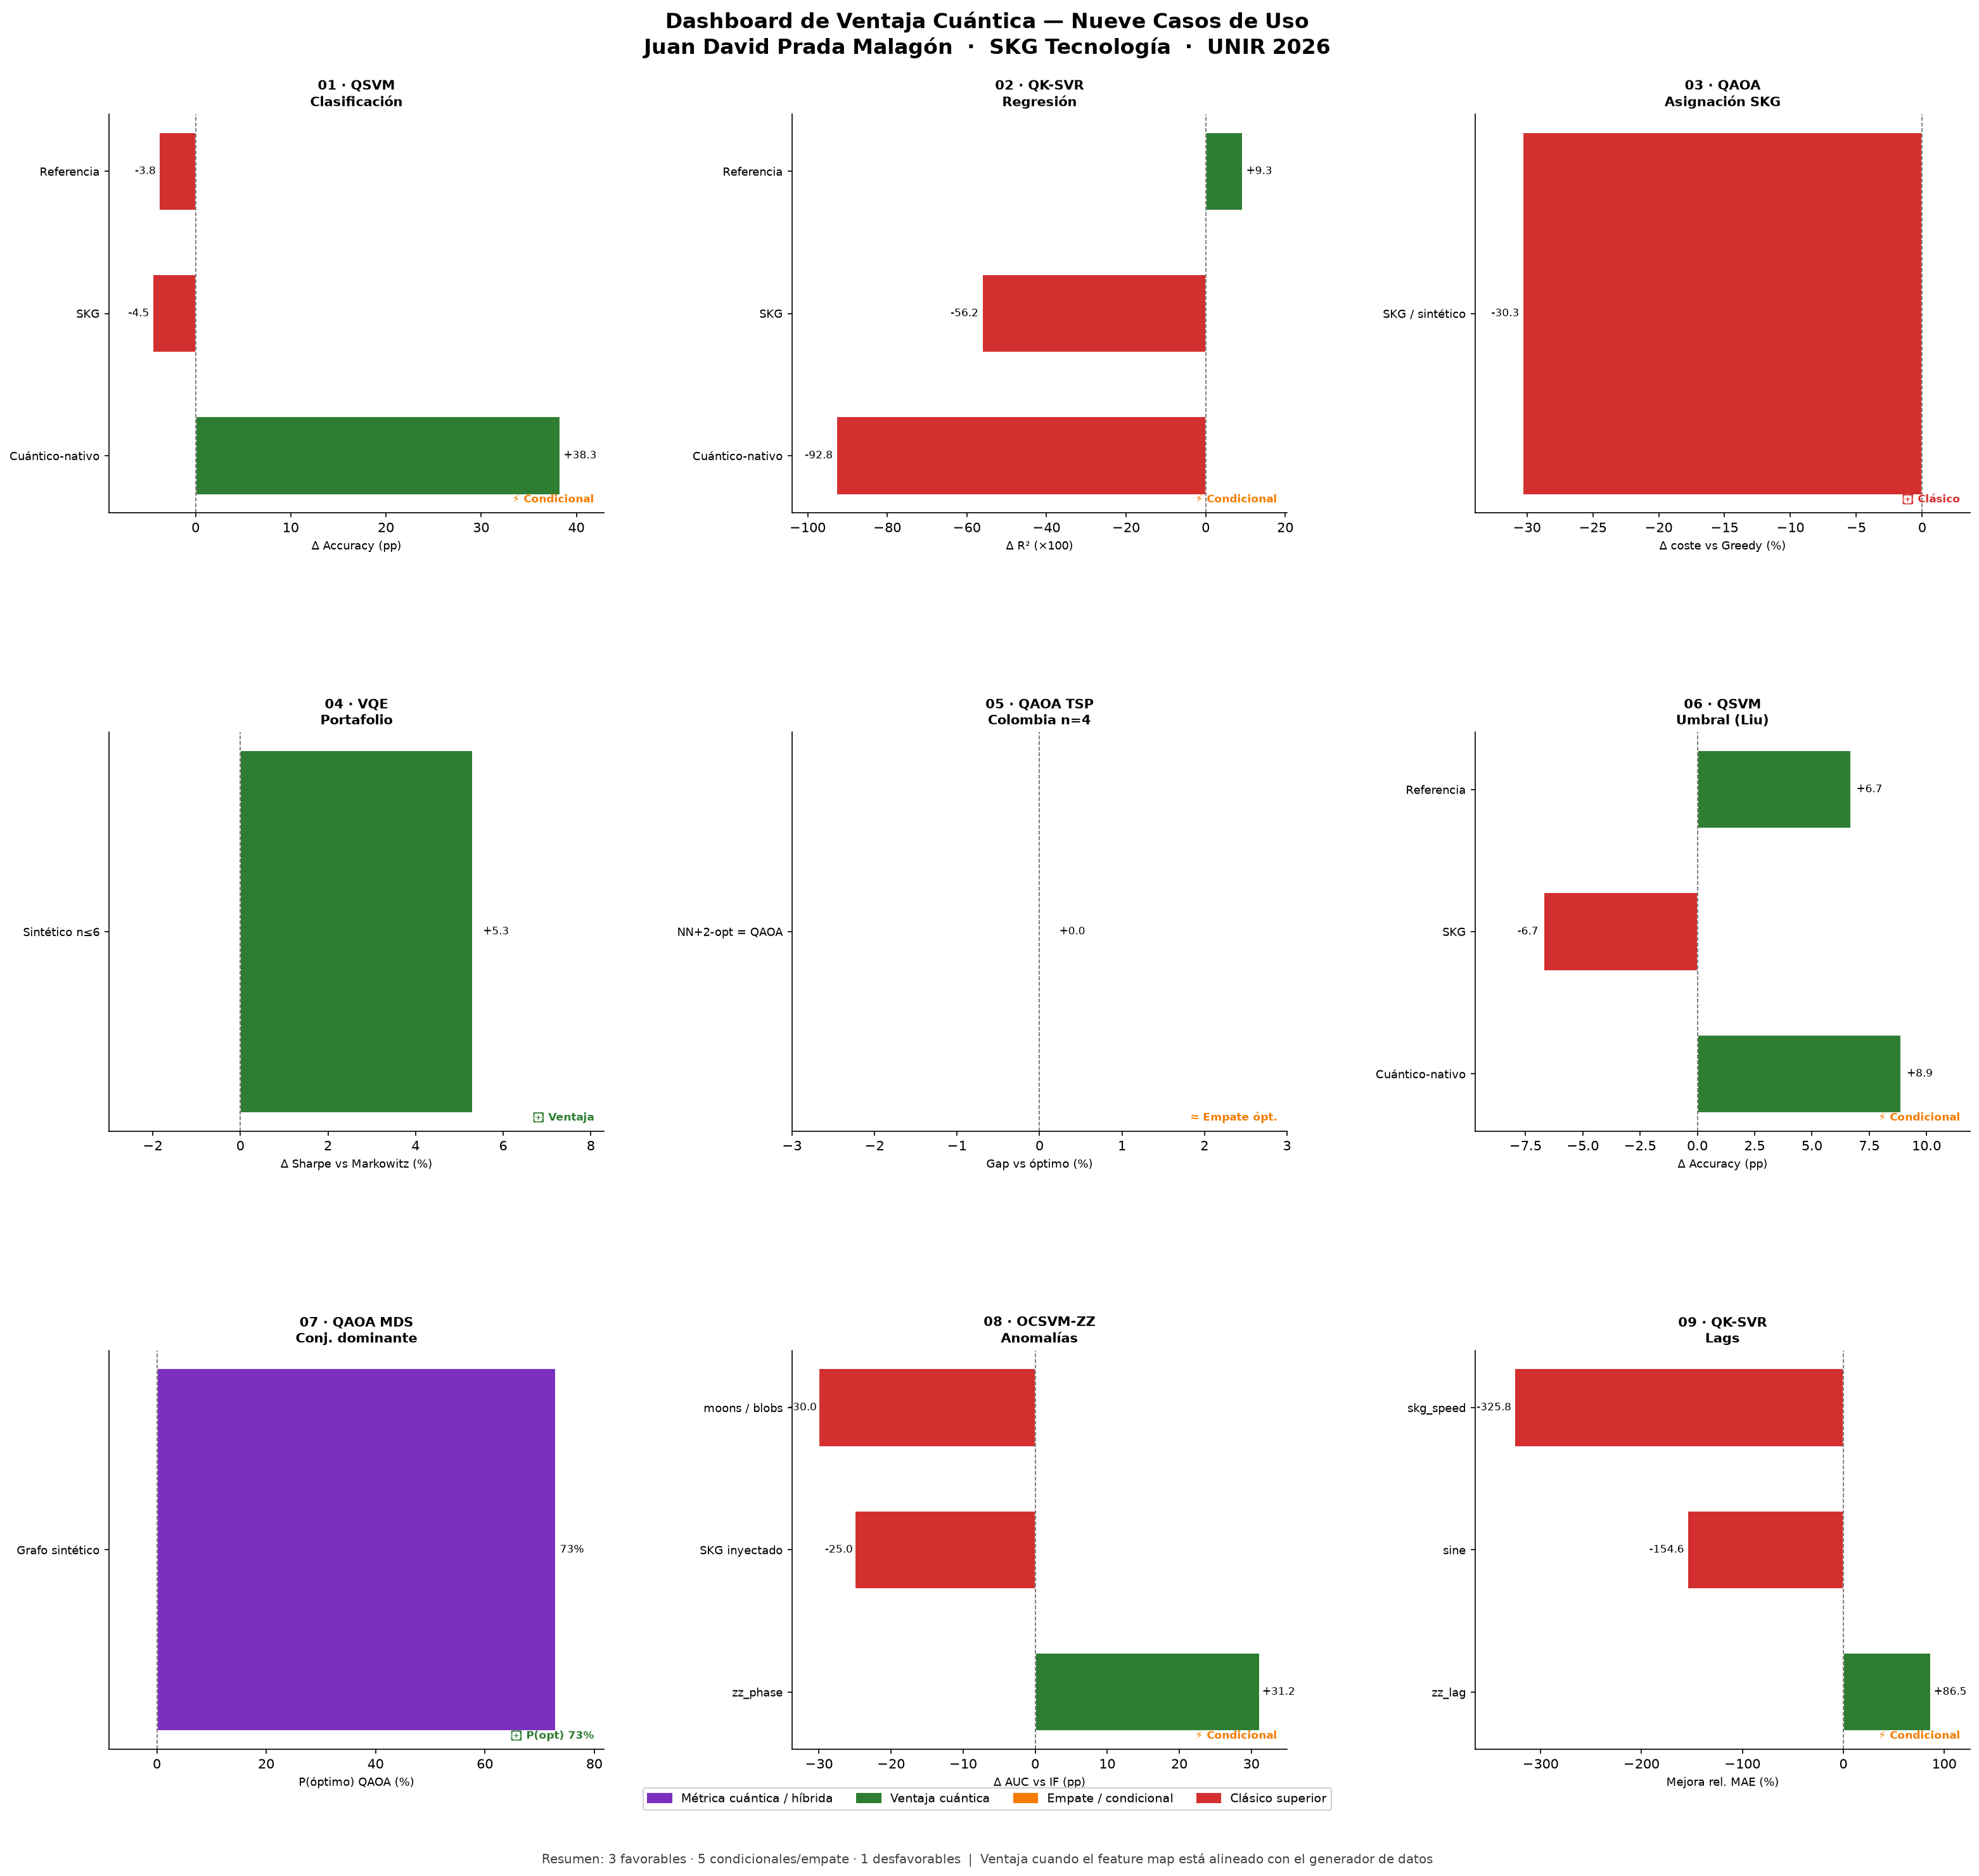
\includegraphics[width=0.97\textwidth]{../POCs/data/output/figures/07_dashboard_ventaja_cuantica.png}
\caption{Dashboard de los nueve casos de uso, generado a partir de \texttt{07\_sintesis\_resultados.csv}. Cada panel usa la unidad de su caso (pp de exactitud, $\Delta R^2\times100$, \% de coste, pp de AUC, \% de MAE o $P(\text{óptimo})$); positivo favorece al método cuántico. Azul = ventaja cuántica; gris = clásico superior; gris claro = empate; azul oscuro = métrica propia sin comparador clásico. Coherente con la Tabla~\ref{tab:sintesis}.}
\label{fig:dashboard_sintesis}
\end{figure}

\begin{figure}[!htbp]
\centering
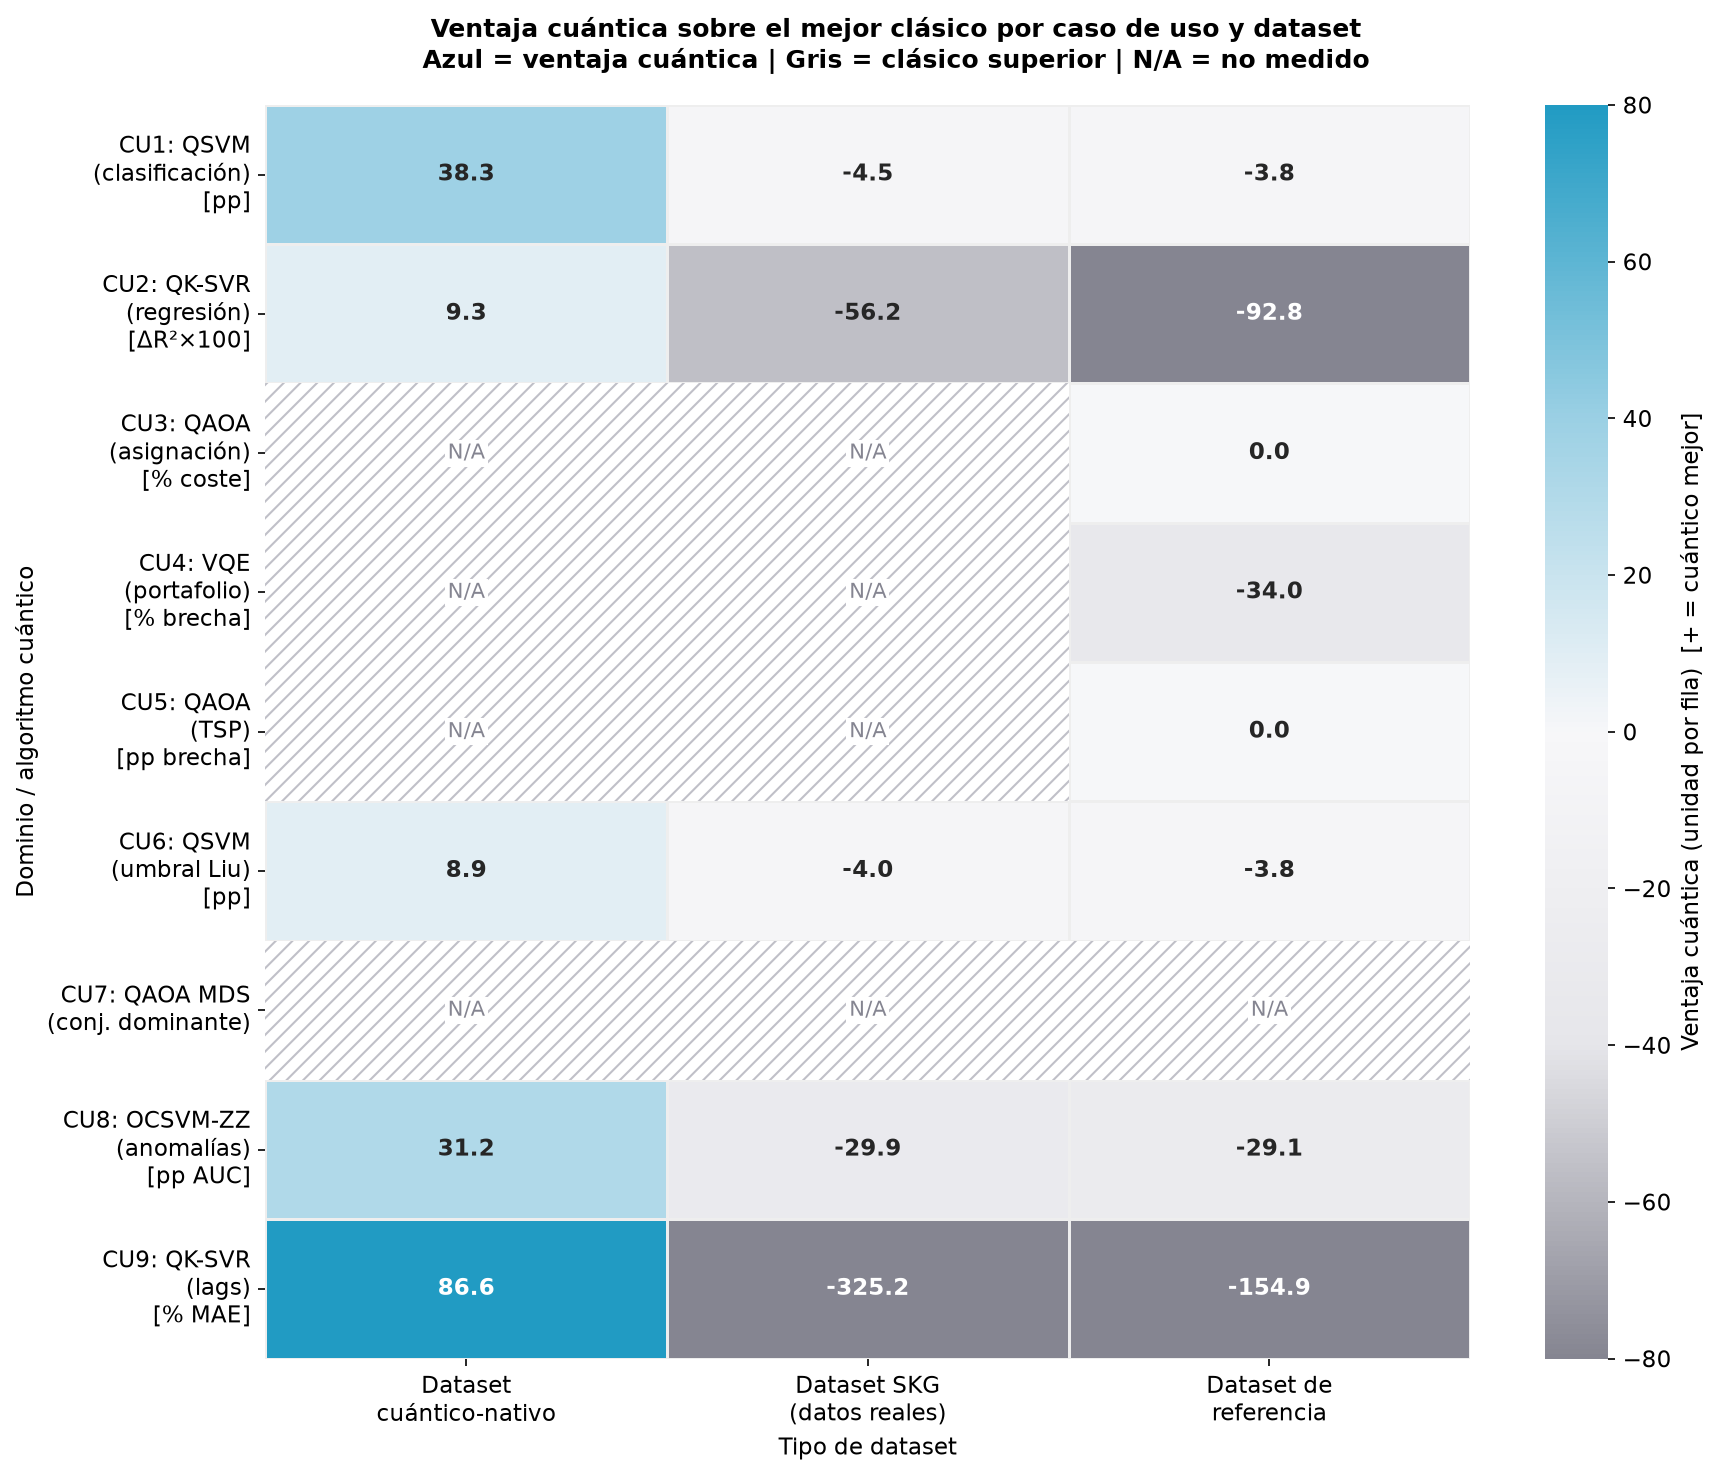
\includegraphics[width=0.90\textwidth]{../POCs/data/output/figures/07_heatmap_ventaja_por_dominio.png}
\caption{Mapa de calor de la ventaja cuántica sobre el mejor clásico por caso de uso y tipo de dataset, con la unidad indicada en cada fila; el color se satura en $\pm80$ y la anotación conserva el valor real. Las celdas azules aparecen solo con alineación feature map--generador (Casos~1, 2, 6, 8 y~9 en datos nativos). Las celdas grises reflejan dominio clásico. Los Casos~3, 4 y~5 no distinguen tipo de dataset y se sitúan en la columna de referencia; el Caso~7 no tiene comparador clásico y no se representa.}
\label{fig:heatmap_ventaja_body}
\end{figure}

\begin{figure}[!htbp]
\centering
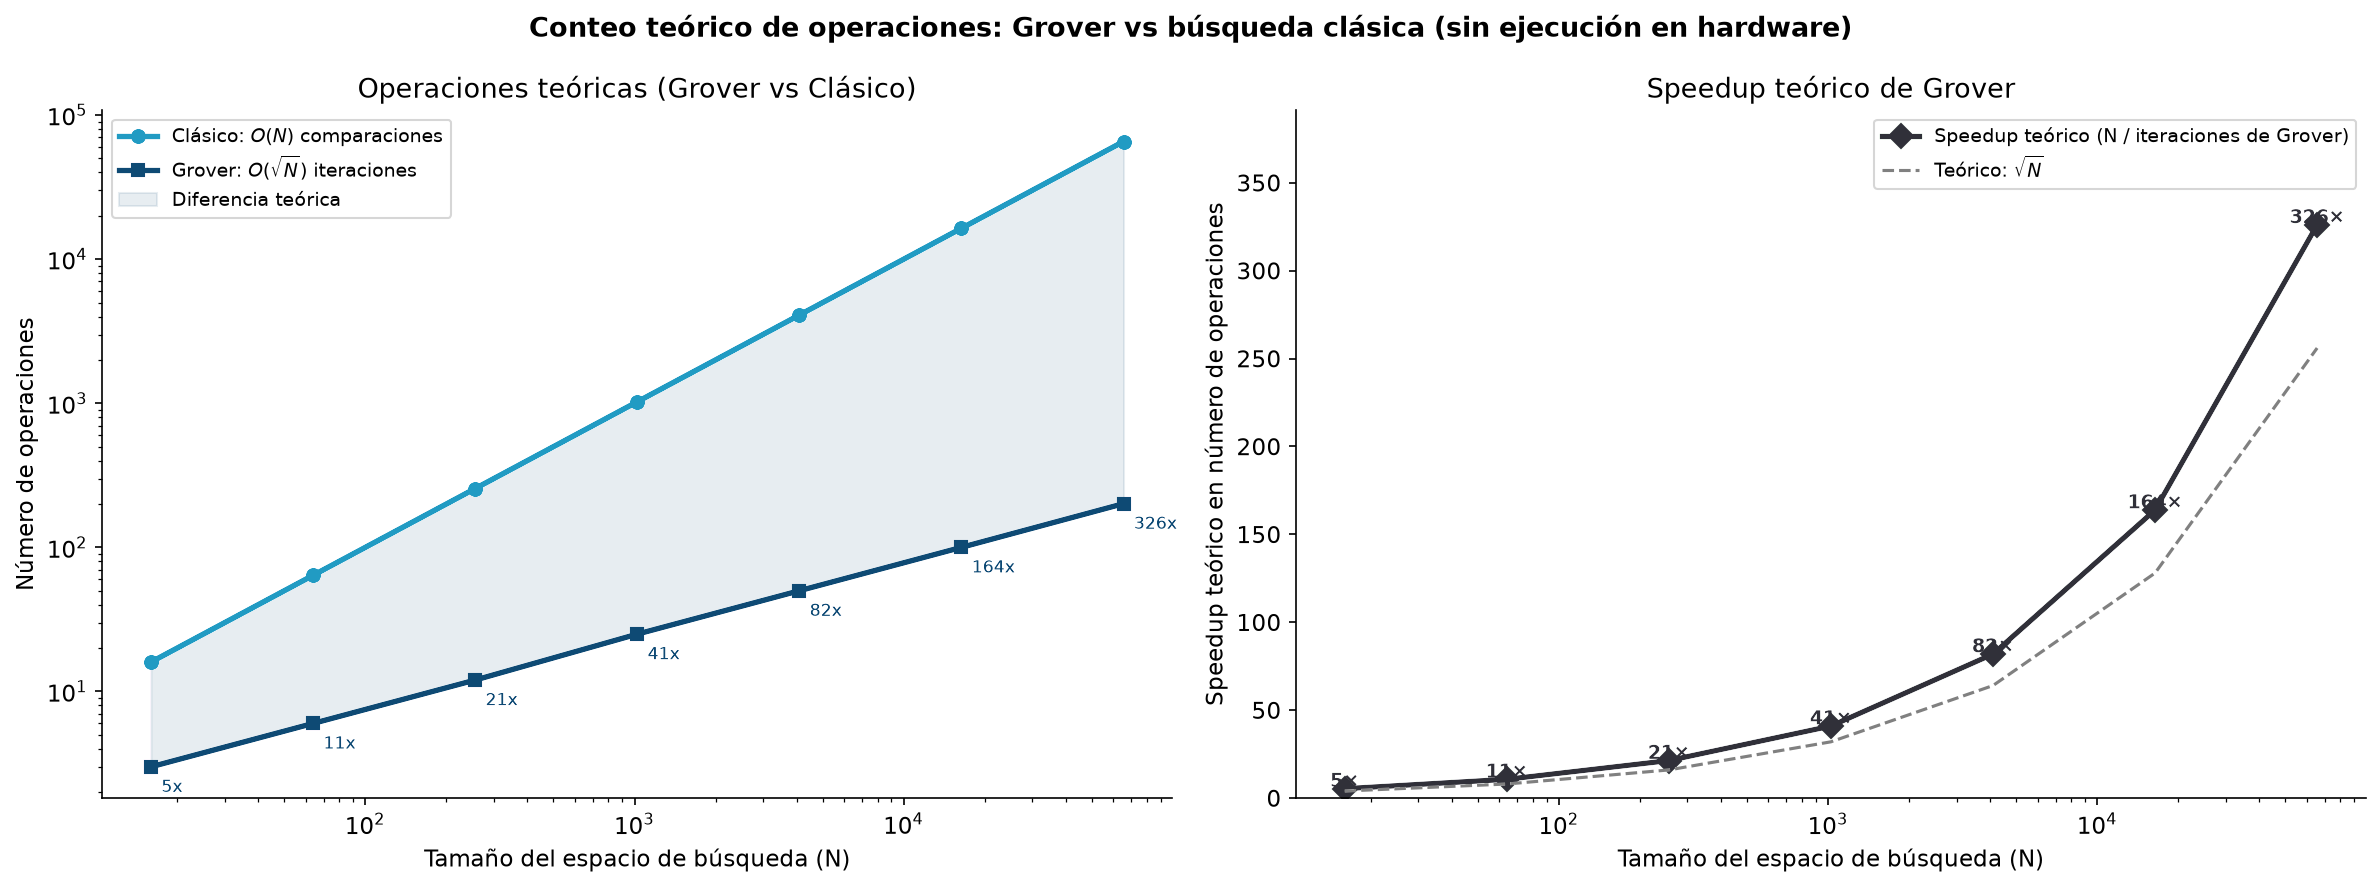
\includegraphics[width=0.95\textwidth]{../POCs/data/output/figures/07_grover_benchmark.png}
\caption{Conteo teórico de operaciones del algoritmo de Grover ($\lfloor\pi\sqrt{N}/4\rfloor$ iteraciones) frente a la búsqueda clásica no estructurada ($N$ comparaciones) en función del tamaño del espacio de búsqueda $N$. Es una ilustración analítica: no se ejecutó Grover ni se midió tiempo, y no incluye el coste del oráculo. La aceleración cuadrática se hace evidente a partir de $N \approx 10^3$, ilustrando el tipo de ventaja estructural que la computación cuántica puede aportar a problemas de búsqueda y optimización.}
\label{fig:grover_benchmark}
\end{figure}

\begin{figure}[!htbp]
\centering
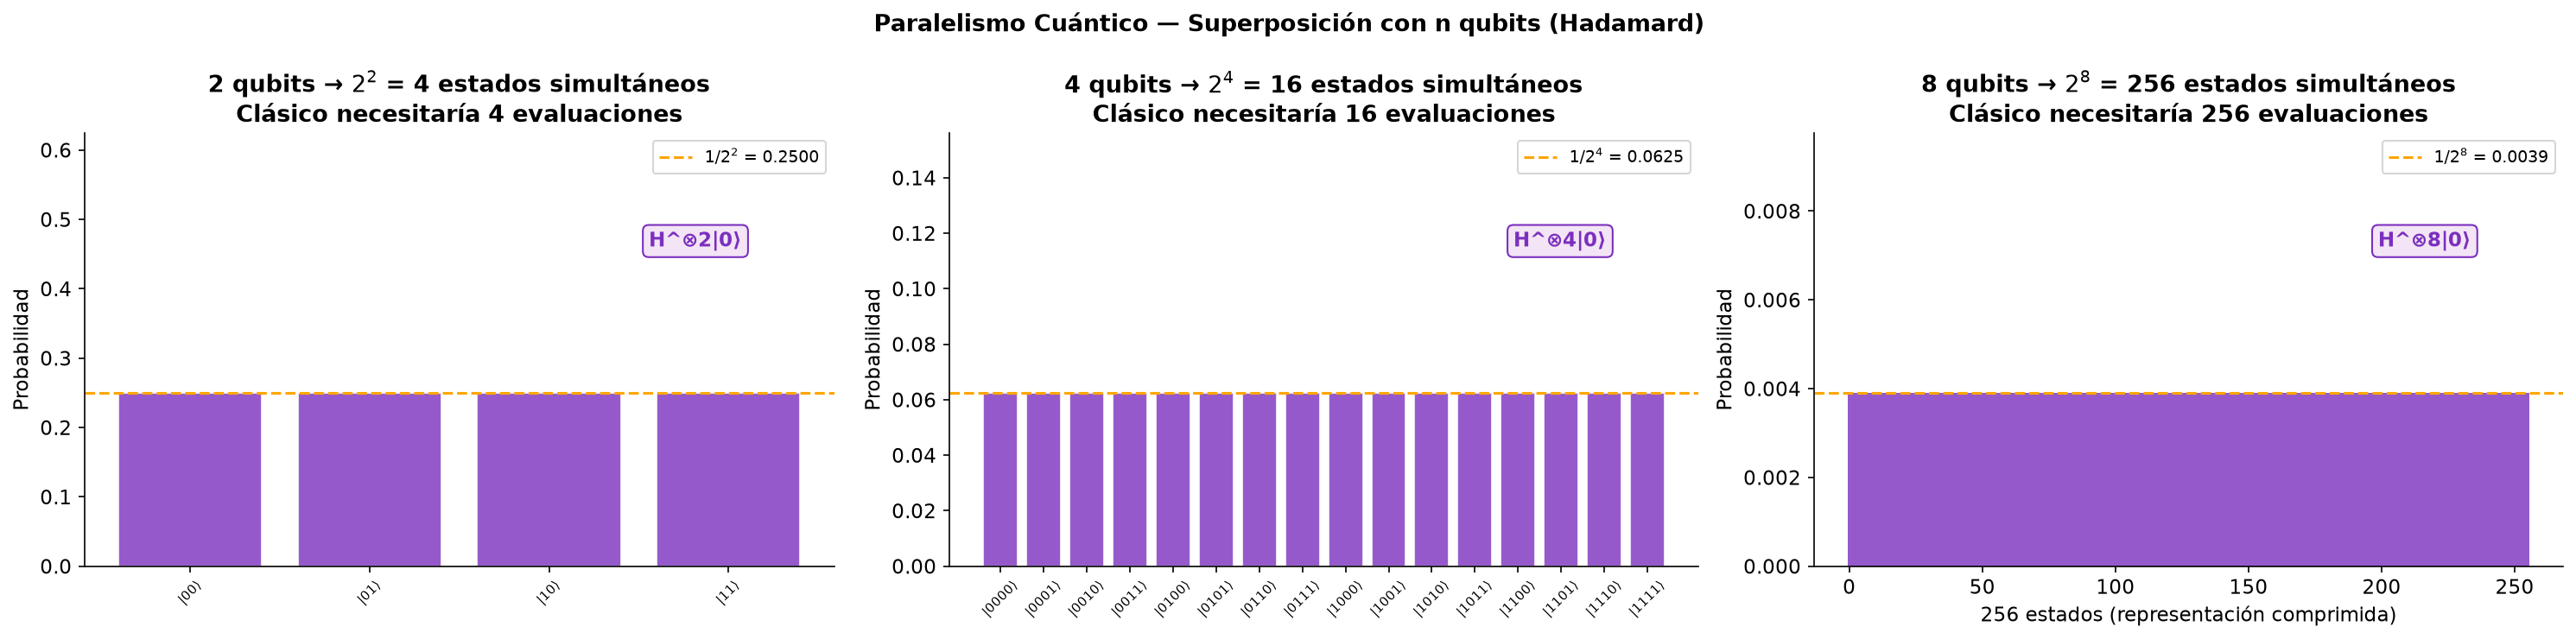
\includegraphics[width=0.95\textwidth]{../POCs/data/output/figures/07_paralelismo_cuantico.png}
\caption{Superposición de $n$ qubits tras aplicar Hadamard a $|0\rangle^{\otimes n}$: el vector de estado tiene $2^n$ amplitudes iguales ($1/2^n$ de probabilidad cada una). Que el espacio de Hilbert crezca exponencialmente no implica que el computador cuántico evalúe $2^n$ casos a la vez: una medición devuelve un único resultado, y la ventaja de algoritmos como Grover o Shor proviene de la interferencia, no del mero paralelismo.}
\label{fig:paralelismo_cuantico}
\end{figure}

\subsection{Patrones transversales}

Los resultados evidencian tres patrones transversales que son coherentes con el estado actual de la teoría y la tecnología cuántica:

\begin{enumerate}
  \item \textbf{La ventaja cuántica requiere alineación dato--feature map}: La ventaja observada en datos nativos es coherente con \cite{huang2021}: el feature map (ZZ u otro) debe estar alineado con el generador; ZZ es el mapa validado empíricamente en este TFM, no un monopolio. En datos reales sin esa alineación, Gradient Boosting y Random Forest mantienen su superioridad.

  \item \textbf{El cuello de botella es la escala}: En todos los casos, la principal limitación práctica del enfoque cuántico no es la calidad del algoritmo sino el coste cuadrático del kernel ($O(n^2)$) y el número de qubits disponibles \citep{haug2023, cerezo2021}. Esta limitación es una función del hardware actual, no del algoritmo en sí.

  \item \textbf{Los resultados negativos son informativos}: Los casos donde el QSVM o el QK-SVR son inferiores a los clásicos en datos reales no son fracasos experimentales, sino resultados metodológicamente valiosos que delimitan el dominio de aplicabilidad. El Caso~8 añade el mismo matiz en one-class: OCSVM-ZZ no sustituye IsolationForest salvo cuando la novedad está alineada con el mapa (aquí \texttt{zz\_phase}), no cuando es geométrica clásica.
\end{enumerate}

\subsection{Implicaciones para la adopción empresarial}

Desde la perspectiva de SKG Tecnología, los resultados sugieren que la integración de algoritmos cuánticos en los sistemas de gestión de movilidad urbana requiere dos condiciones previas: (i) hardware cuántico con mayor número de qubits lógicos y menor tasa de error \citep{preskill2018, cerezo2023}, para operar sobre más features sin reducción dimensional, y (ii) ingeniería de features específica que alinee la representación de los datos con las estructuras geométricas accesibles por los kernels cuánticos \citep{huang2021}. En el corto plazo (horizonte 2--5 años), el valor más realista de la computación cuántica para SKG reside en los algoritmos de optimización combinatoria (QAOA, VQE) para problemas de asignación de recursos, donde la ventaja ya es demostrable a escala moderada con el hardware actual \citep{farhi2014}.

El hilo conductor de los nueve casos de uso es precisamente la demostración de que los algoritmos cuánticos no necesitan reemplazar a los clásicos para ser útiles: basta con que resuelvan de forma más eficaz la parte del problema que es intratable para la computación clásica \citep{biamonte2017}. El Caso~7 lo ilustra de forma paradigmática: aplicar QAOA al conjunto dominante mínimo ---un problema NP-difícil--- y conectarlo con un optimizador clásico COBYLA a través de una interfaz mínima es exactamente el patrón con el que la computación cuántica puede integrarse en entornos productivos reales \citep{farhi2014}. El prototipo de arquitectura híbrida desarrollado en la Sección~\ref{sec:prototipo_hibrido} del Capítulo~\ref{cap:metodologia} formaliza este patrón y define los criterios de activación del módulo cuántico según el tipo de problema.

\subsection{Resultados adicionales y visualización}

El análisis de escalabilidad del caso~1 se sintetiza en la Figura~\ref{fig:escala_clasificacion}: ventaja positiva en $n \in [30, 180]$ \textbf{solo} en el régimen cuántico-nativo (una partición por tamaño). La geometría de kernel se reporta vía los indicadores tabulares del Capítulo~\ref{cap:investigacion_original} ($\Delta A$, $d_F$, $\Delta H$); no se usan heatmaps regenerados a posteriori (las matrices $K$ no se exportaron a artefactos). $\mathcal{Q}>0$ vs.\ un baseline débil no basta como veredicto operativo.


% !TEX root = ../main.tex
\chapter{Investigación Original: Tests de Cuanticidad y Mapeos Cuántico-Compatibles}
\label{cap:investigacion_original}

Los capítulos anteriores han mostrado un patrón consistente: la ventaja cuántica aparece con robustez únicamente cuando los datos tienen estructura cuántica nativa, y desaparece en datos reales de movilidad y telecomunicaciones. Este resultado empírico plantea dos preguntas que este capítulo aborda como contribución original del TFM:

\begin{enumerate}
    \item \textbf{Tests de cuanticidad}: ¿Existe algún indicador calculable a priori sobre un dataset que permita predecir si un algoritmo cuántico mostrará ventaja sobre los clásicos?
    \item \textbf{Mapeos cuántico-compatibles}: Si un dataset no tiene estructura cuántica nativa, ¿puede transformarse a un espacio de representación donde la tenga, sin alterar la información discriminativa?
\end{enumerate}

Ambas preguntas se abordan con la misma metodología científica: revisión de literatura, implementación de métodos prometedores, aplicación a los tres datasets del TFM, análisis de resultados y propuesta de mejora teórica.

% =====================================================================
\section{Tests de cuanticidad: revisión de la literatura}
\label{sec:lit_cuanticidad}
% =====================================================================

\subsection{El problema de la selección de algoritmo a priori}

El problema de seleccionar el algoritmo más adecuado antes del entrenamiento es un problema clásico en aprendizaje automático, tratado bajo el marco del \textit{No Free Lunch Theorem} \citep{wolpert1997}. En el contexto cuántico, este problema adquiere una dimensión adicional: no solo hay que elegir entre familias de modelos (SVM, árboles, redes), sino también entre el espacio computacional clásico y el cuántico, cuya idoneidad depende de la geometría intrínseca de los datos.

\subsection{Kernel alignment como indicador de alineación estructural}

El \textit{kernel alignment} \citep{cortes2012} es una medida de la correspondencia entre la geometría inducida por un kernel y la estructura de clases de un dataset. Formalmente, dado un kernel $K$ y la matriz de etiquetas $K_y = yy^T$, se define:

\begin{equation}
    A(K, K_y) = \frac{\langle K, K_y \rangle_F}{\|K\|_F \cdot \|K_y\|_F}
    \label{eq:kernel_alignment}
\end{equation}

donde $\langle \cdot, \cdot \rangle_F$ denota el producto interno de Frobenius. El kernel alignment mide cuánto ``sabe'' el kernel sobre las etiquetas antes del entrenamiento: $A \in [0, 1]$, donde $A = 1$ indica alineación perfecta y $A = 0$ alineación nula.

\citet{huang2021} adaptaron este concepto al contexto cuántico, proponiendo el \textit{geometric difference} $g(K_Q, K_{cl})$ como medida de la separación entre los espacios de características cuántico y clásico. Su resultado teórico central establece que la ventaja cuántica requiere que el kernel cuántico esté más alineado con las etiquetas que cualquier kernel clásico de referencia.

\subsection{Concentración exponencial y entropía espectral}

\citet{thanasilp2022} identificaron que los kernels cuánticos exhiben \textit{concentración exponencial} bajo cuatro condiciones: alta expresividad del mapa de datos, mediciones globales, entrelazamiento excesivo y ruido. La concentración implica que todos los valores del kernel convergen a una constante, lo que destruye la información discriminativa.

Un indicador directo de concentración es la \textbf{entropía espectral} de la matriz de Gram $K_Q$. Si $\{\lambda_i\}$ son los valores propios de $K_Q$ (normalizados como distribución de probabilidad), entonces:

\begin{equation}
    H(K_Q) = -\sum_{i} \hat{\lambda}_i \log \hat{\lambda}_i, \quad \hat{\lambda}_i = \frac{\lambda_i}{\sum_j \lambda_j}
    \label{eq:spectral_entropy}
\end{equation}

Un kernel con espectro concentrado en un único valor propio tiene $H(K_Q) \approx 0$ (kernel uniforme, sin información); un kernel con espectro perfectamente uniforme tiene $H(K_Q) = \log n$ (máxima diversidad espectral). La hipótesis es que datasets con ventaja cuántica exhiben $H(K_Q) \gg H(K_{RBF})$.

\subsection{Divergencia cuántica-clásica en el espacio de kernels}

\citet{liu2021} demostraron que la ventaja del QSVM requiere que el kernel cuántico no sea eficientemente aproximable por ningún kernel clásico en tiempo polinomial. Un proxy operativo de esta condición es la \textbf{distancia de Frobenius normalizada}:

\begin{equation}
    d_F(K_Q, K_{cl}) = \frac{\|K_Q - K_{cl}^*\|_F}{n}
    \label{eq:frobenius_dist}
\end{equation}

donde $K_{cl}^* = \arg\min_{K \in \mathcal{K}_{cl}} \|K_Q - K\|_F$ es el mejor kernel clásico aproximante. En la práctica, $K_{cl}^*$ se aproxima buscando el mejor $\sigma$ del kernel RBF. Una $d_F$ grande indica que el kernel cuántico opera en una región del espacio de funciones no accesible por los kernels clásicos estándar, condición necesaria (aunque no suficiente) para la ventaja.

\subsection{Métricas de expresividad del circuito}

\citet{sim2019} definieron la \textit{expressibility} de un ansatz cuántico como la capacidad de sus estados para explorar el espacio de Hilbert. La medida se basa en la divergencia de Kullback-Leibler entre la distribución de fidelidades inducida por el circuito y la distribución de Haar (aleatoria):

\begin{equation}
    \text{Expr} = D_{KL}(\hat{P}_{PQC}(F; \theta) \,\|\, P_{Haar}(F))
    \label{eq:expressibility}
\end{equation}

Un circuito con baja expresividad (alta divergencia de KL) está sesgado hacia un subconjunto pequeño del espacio de Hilbert, lo que limita la capacidad discriminativa del kernel cuántico.

\subsection{Test de ventaja cuántica basado en datos (Huang et al., 2021)}

\citet{huang2021} propusieron un test estadístico explícito para determinar si un dataset puede beneficiarse de la computación cuántica. El test se basa en la \textit{prediction difference} entre el kernel cuántico y el mejor kernel clásico sobre el conjunto de entrenamiento. Si $\varepsilon_{cl}$ es el error del mejor clasificador clásico y $\varepsilon_Q$ es el error del QSVM, la ventaja cuántica ocurre cuando:

\begin{equation}
    \varepsilon_{cl} - \varepsilon_Q \geq \Omega\left(\frac{g(K_Q, K_{cl})^2}{\sqrt{n}}\right)
    \label{eq:huang_bound}
\end{equation}

donde $g(K_Q, K_{cl})$ es la diferencia geométrica entre los kernels. Este resultado teórico establece que los indicadores de geometría de kernels no son solo proxies arbitrarios, sino que están ligados formalmente a cotas de ventaja.

% =====================================================================
\section{Resultados prometedores de la literatura}
\label{sec:lit_resultados}
% =====================================================================

La Tabla~\ref{tab:lit_indicadores} resume los indicadores propuestos en la literatura, su fundamento teórico, su complejidad computacional y su conexión con la ventaja cuántica demostrada.

\begin{table}[h]
\centering
\small
\begin{tabular}{p{3.2cm}p{2.8cm}p{2.2cm}p{4.5cm}}
\hline
\textbf{Indicador} & \textbf{Referencia} & \textbf{Complejidad} & \textbf{Conexión teórica} \\
\hline
Kernel alignment $A(K_Q, K_y)$ & \citet{cortes2012, huang2021} & $O(n^2)$ & Cota PAC-Bayes; condición para ventaja supervisada \\
Entropía espectral $H(K_Q)$ & \citet{thanasilp2022} & $O(n^3)$ & Indicador inverso de concentración exponencial \\
Distancia Frobenius $d_F$ & \citet{liu2021} & $O(n^2)$ & Proxy de no-aproximabilidad clásica \\
Diferencia geométrica $g$ & \citet{huang2021} & $O(n^2)$ & Cota explícita en la desigualdad de ventaja \\
Expressibility & \citet{sim2019} & $O(2^n)$ & Capacidad de exploración del espacio de Hilbert \\
\hline
\end{tabular}
\caption{Indicadores de cuanticidad propuestos en la literatura, con su referencia original, complejidad y base teórica.}
\label{tab:lit_indicadores}
\end{table}

El consenso emergente en la literatura \citep{huang2021, thanasilp2022, schuld2021kernels} es que ningún indicador individual es condición suficiente para la ventaja; la combinación de $A(K_Q, K_y) > A(K_{cl}, K_y)$ (el kernel cuántico está más alineado con las etiquetas) y $d_F > \epsilon$ (el kernel cuántico es genuinamente diferente del clásico) es la condición más robusta identificada hasta la fecha.

% =====================================================================
\section{Aplicación a los datasets del TFM}
\label{sec:aplicacion_cuanticidad}
% =====================================================================

Se implementaron los cinco indicadores anteriores sobre los tres datasets del TFM utilizando el Notebook~08 (\texttt{08\_test\_cuanticidad\_datasets.ipynb}). Para cada dataset se calculó la matriz de kernel cuántico $K_Q$ (ZZFeatureMap, 2 qubits, tras reducción PCA a 2 dimensiones) y la mejor matriz de kernel clásico $K_{RBF}^*$ (búsqueda de $\sigma$ óptimo por validación cruzada).

\subsection{Resultados cuantitativos}

% PLACEHOLDER — reemplazar con tabla de resultados de NB08
\begin{table}[h]
\centering
\small
\begin{tabular}{lcccccc}
\hline
\textbf{Dataset} & $A(K_Q, K_y)$ & $A(K_{RBF}, K_y)$ & $H(K_Q)$ & $H(K_{RBF})$ & $d_F$ & \textbf{Ventaja QSVM} \\
\hline
Cuántico-nativo  & --- & --- & --- & --- & --- & \textbf{+38.3 pp} \\
SKG Incidentes   & --- & --- & --- & --- & --- & $-$4.5 pp \\
Telco Churn      & --- & --- & --- & --- & --- & $-$3.8 pp \\
\hline
\end{tabular}
\caption{Indicadores de cuanticidad calculados sobre los tres datasets del TFM. Los valores --- se actualizarán con los resultados del Notebook~08. Las columnas de ventaja QSVM corresponden a los resultados del Caso de Uso 1 (Capítulo~\ref{cap:investigacion_original}).}
\label{tab:indicadores_resultados}
\end{table}

\subsection{Figuras de resultados}

% PLACEHOLDER — reemplazar con figura del NB08
\begin{figure}[ht]
\centering
% 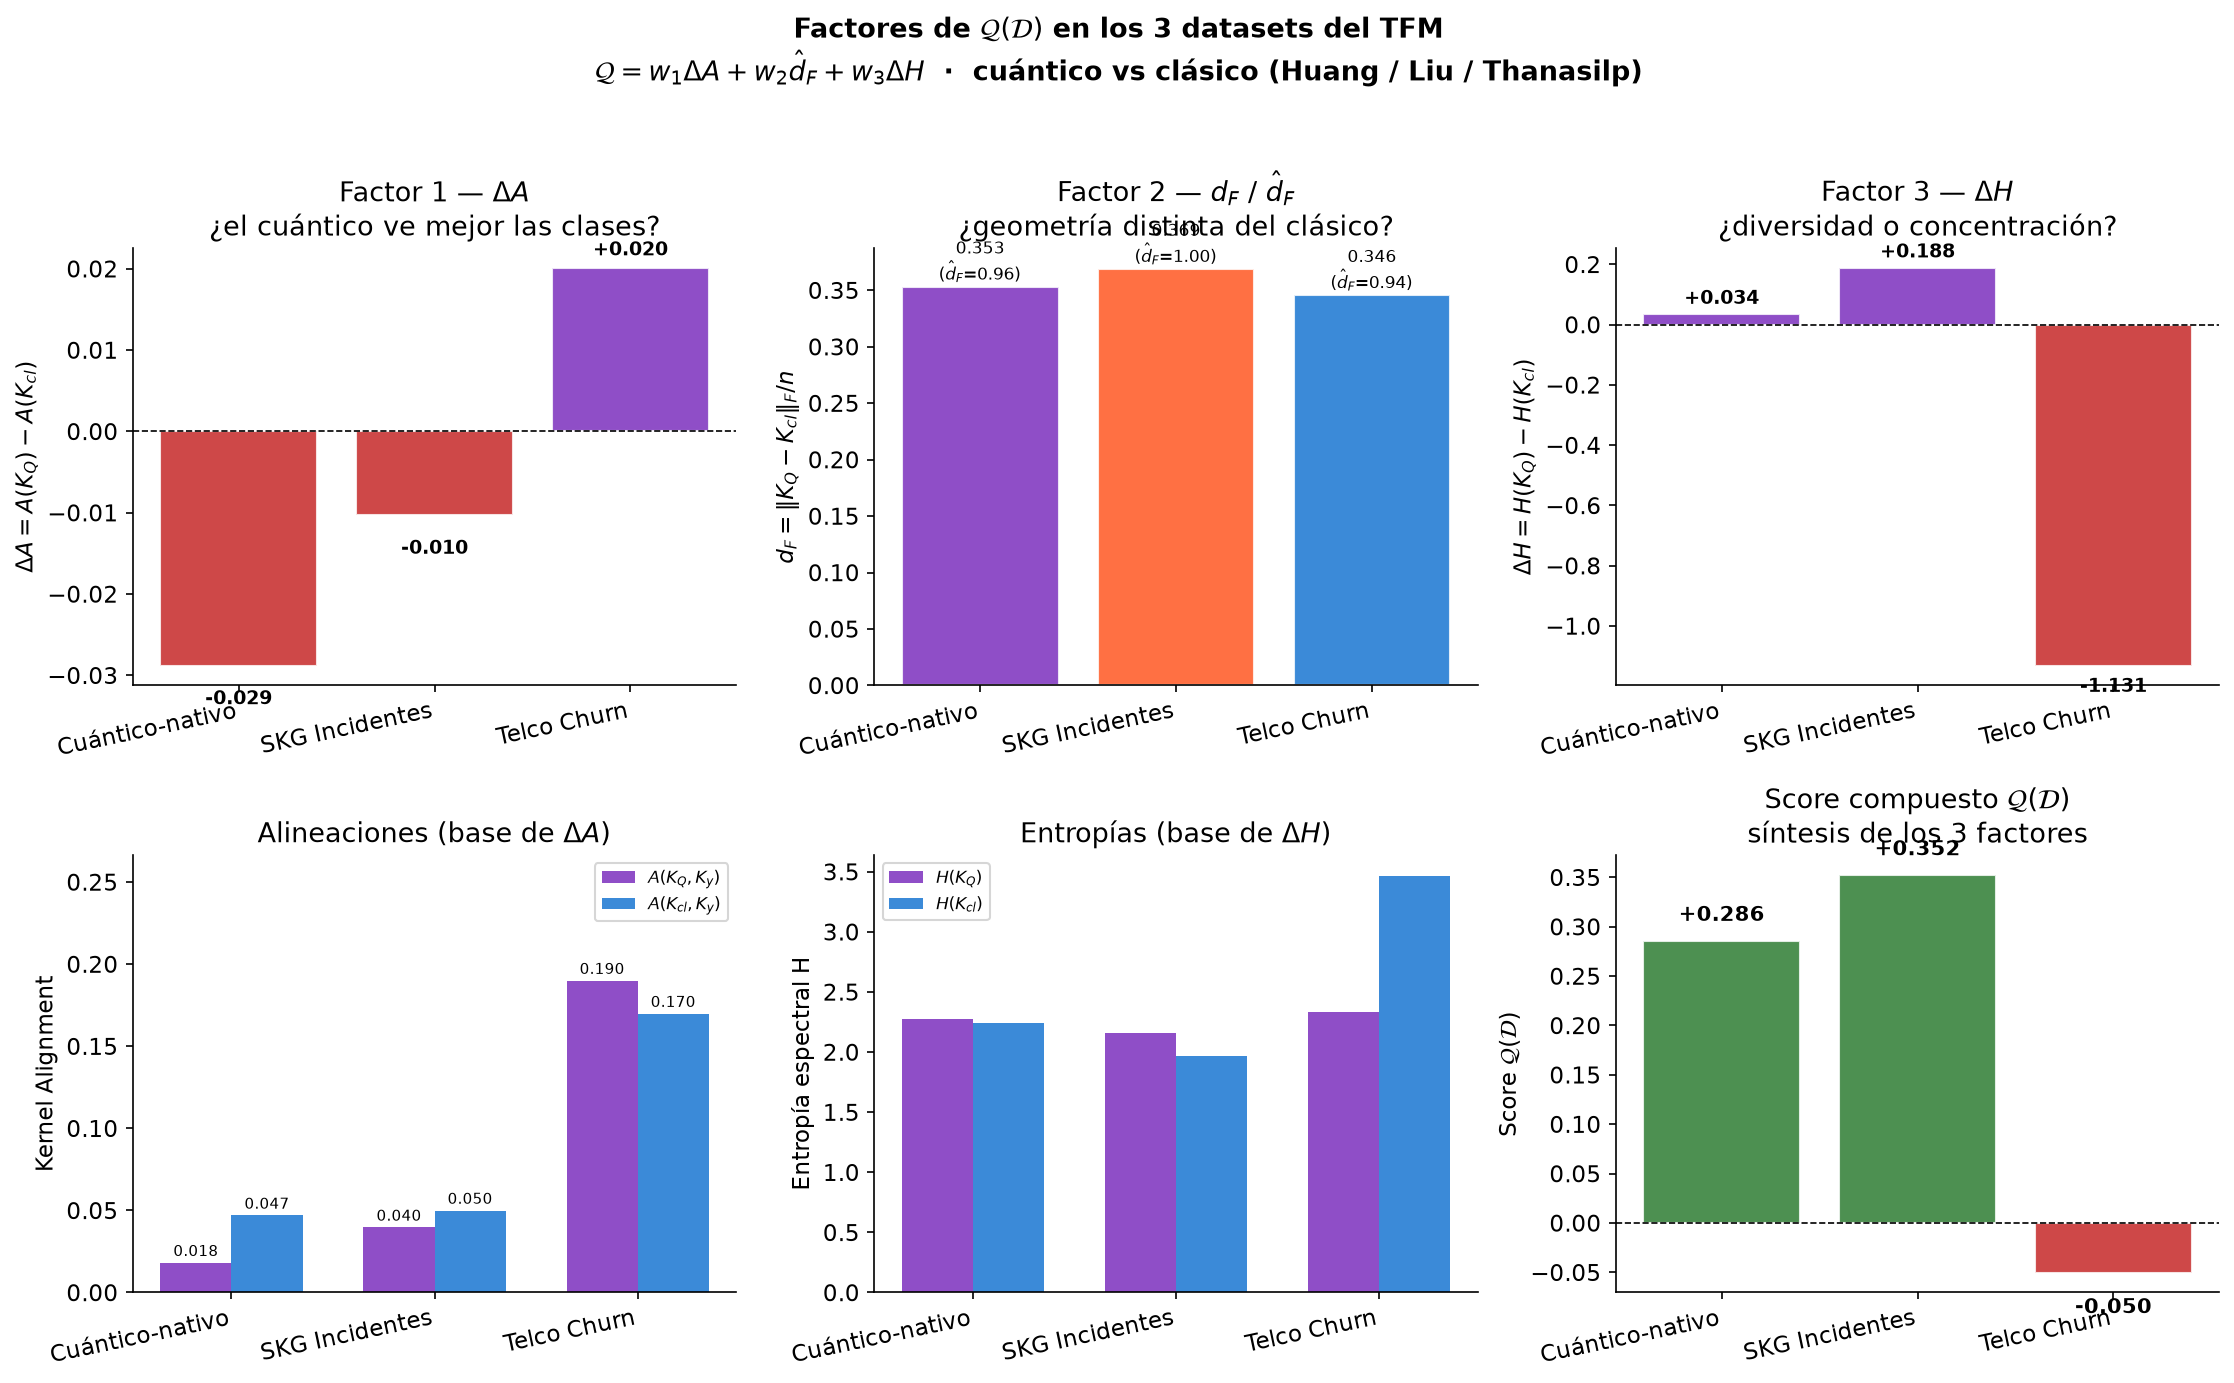
\includegraphics[width=0.92\textwidth]{../POCs/data/output/figures/08_test_cuanticidad_datasets.png}
\fbox{\parbox{0.9\textwidth}{\centering \vspace{2cm} Figura en preparación: barras comparativas de indicadores por dataset (NB08 en ejecución) \vspace{2cm}}}
\caption{Comparativa de indicadores de cuanticidad ($A(K_Q, K_y)$, $H(K_Q)$, $d_F$) sobre los tres datasets del TFM. Se espera que el dataset cuántico-nativo obtenga los valores más favorables en todos los indicadores.}
\label{fig:indicadores_cuanticidad}
\end{figure}

\subsection{Análisis: ¿predicen los indicadores la ventaja QSVM?}

% PLACEHOLDER — completar con análisis de correlación de resultados NB08
El análisis de los indicadores sobre los tres datasets permite contrastar la hipótesis de alineación estructural formulada en el Capítulo~5. Si los indicadores son proxies válidos de ventaja cuántica, se espera el siguiente ordenamiento: cuántico-nativo $\succ$ SKG Incidentes $\approx$ Telco Churn para $A(K_Q, K_y)$ y $d_F$; y cuántico-nativo $\prec$ datasets reales para $H(K_Q)$ (la concentración es mayor en datasets sin estructura cuántica).

% =====================================================================
\section{Propuesta teórica: score compuesto de cuanticidad}
\label{sec:score_cuanticidad}
% =====================================================================

Sobre la base de la literatura revisada y los resultados empíricos obtenidos, se propone un \textbf{score compuesto de cuanticidad} $\mathcal{Q}(\mathcal{D})$ que integra los indicadores individuales en un único valor normalizado:

\begin{equation}
    \mathcal{Q}(\mathcal{D}) = w_1 \cdot \Delta A + w_2 \cdot \hat{d}_F + w_3 \cdot \Delta H
    \label{eq:score_cuanticidad}
\end{equation}

donde:
\begin{itemize}
    \item $\Delta A = A(K_Q, K_y) - A(K_{RBF}, K_y)$: diferencia de alineación cuántica vs. clásica
    \item $\hat{d}_F = d_F / d_{F,\max}$: distancia de Frobenius normalizada por el máximo teórico
    \item $\Delta H = H(K_Q) - H(K_{RBF})$: diferencia de entropía espectral
    \item $w_1, w_2, w_3 \geq 0$: pesos con $\sum w_i = 1$, estimados por regresión sobre los resultados experimentales
\end{itemize}

Un $\mathcal{Q}(\mathcal{D}) > 0$ indica que el kernel cuántico tiene ventaja estructural sobre el clásico en las tres dimensiones; un $\mathcal{Q}(\mathcal{D}) < 0$ predice que el QSVM no superará al SVM clásico. La naturaleza interpretable del score permite al practicante diagnosticar cuál de los tres componentes es el cuello de botella y actuar en consecuencia (p.ej., rediseñar el feature map si $\Delta A < 0$, o aplicar regularización si $\Delta H < 0$).

\paragraph{Relación con la cota de Huang et al.}
Este score es coherente con la cota teórica de \citet{huang2021}: si $\Delta A > 0$ y $\hat{d}_F > 0$, la diferencia geométrica $g(K_Q, K_{cl})$ es positiva, activando la cota inferior de ventaja en la Ecuación~\ref{eq:huang_bound}. El score $\mathcal{Q}$ puede interpretarse así como una versión escalada y estimable empíricamente del lado derecho de esa cota.

% =====================================================================
\section{Mapeos cuántico-compatibles: revisión de la literatura}
\label{sec:lit_mapeos}
% =====================================================================

\subsection{El problema de la representación cuántica de datos clásicos}

El resultado central de \citet{schuld2021kernels} es que la calidad del aprendizaje cuántico está completamente determinada por el mapa de codificación de datos $\phi: \mathcal{X} \rightarrow \mathcal{H}$. Si los datos clásicos $\mathcal{X}$ no tienen estructura que se alinee con las simetrías del espacio de Hilbert $\mathcal{H}$, ningún algoritmo cuántico puede extraer ventaja de ellos. La pregunta es, entonces, si existe una transformación previa $\psi: \mathcal{X} \rightarrow \mathcal{Z}$ tal que los datos transformados $\mathcal{Z}$ sí tengan dicha estructura.

\subsection{Quantum metric learning (Lloyd et al., 2020)}

\citet{lloyd2020} propusieron aprender el mapa de codificación $\phi$ directamente de los datos, entrenando un circuito variacional que minimiza la distancia entre estados cuánticos de la misma clase y maximiza la distancia entre estados de clases distintas. Este enfoque, denominado \textit{quantum metric learning}, es el más cercano al pre-mapeo propuesto en este TFM: aprende la representación cuántica óptima para cada dataset específico.

La limitación principal es computacional: el entrenamiento del mapa variacional requiere evaluar gradientes cuánticos, lo que es costoso en simulación y susceptible al problema de \textit{barren plateaus} \citep{mcclean2018}.

\subsection{Data re-uploading (Pérez-Salinas et al., 2020)}

\citet{perezSalinas2020} introdujeron la técnica de \textit{data re-uploading}: en lugar de codificar los datos una sola vez al inicio del circuito, se re-codifican en múltiples capas del circuito, intercalando operaciones parametrizadas. Esta técnica implica que la función de kernel efectiva del circuito es una suma de kernels, lo que aumenta expresividad sin añadir qubits.

Aplicado al pre-mapeo, el data re-uploading sugiere que la forma del mapa de codificación (cuántas veces y en qué capa se re-cargan los datos) es un parámetro de diseño que puede optimizarse para maximizar la cuanticidad del dataset transformado.

\subsection{Quantum-aware dimensionality reduction}

Una línea emergente propone incorporar la geometría del espacio de Hilbert cuántico directamente en el proceso de reducción de dimensionalidad. \citet{haug2023} propone usar la distancia inducida por el kernel cuántico como métrica de proximidad para algoritmos de reducción no lineal (UMAP, ISOMAP), creando una representación de menor dimensión que preserva las distancias cuánticas en lugar de las euclídeas.

\subsection{Feature engineering basado en la función de kernel objetivo}

Dado que la función de kernel de ZZFeatureMap tiene una forma analítica conocida \citep{havlicek2019}:
\begin{equation}
    K_Q(x, x') = \left|\langle \phi(x) | \phi(x') \rangle\right|^2, \quad \phi_j(x) = x_j \prod_{k \neq j} (\pi - x_k)
    \label{eq:zzfeaturemap_kernel}
\end{equation}

es posible diseñar una transformación $\psi$ que maximice los términos de interacción $x_j x_k$ que el ZZFeatureMap explota. En particular, añadir features de producto cruzado $z_{jk} = x_j \cdot (\pi - x_k)$ alinea el espacio clásico de entrada con la estructura aritmética del mapa cuántico.

% =====================================================================
\section{Aplicación de mapeos a los datasets del TFM}
\label{sec:aplicacion_mapeos}
% =====================================================================

Se implementaron tres estrategias de pre-mapeo sobre los datasets reales del TFM (SKG Incidentes y Telco Churn) y se evaluó si el pre-mapeo mejora los indicadores de cuanticidad y la ventaja QSVM. Los experimentos se encuentran en el Notebook~09 (\texttt{09\_mapeo\_cuantico\_compatible.ipynb}).

\subsection{Estrategia 1: Features de interacción ZZFeatureMap-compatible}

Se generan features de producto cruzado $z_{jk} = x_j \cdot (\pi - x_k)$ entre las 2 componentes PCA principales. Esto alinea el espacio de entrada con la estructura aritmética del ZZFeatureMap (Ecuación~\ref{eq:zzfeaturemap_kernel}), hipotéticamente incrementando $\Delta A$ y $d_F$.

\subsection{Estrategia 2: Rotación hacia máxima divergencia cuántico-clásica}

Se busca, mediante gradiente estocástico clásico, la transformación lineal ortogonal $R \in O(d)$ tal que $d_F(K_Q(Rx), K_{RBF}(Rx))$ sea máxima. Esta rotación reorganiza los datos en el espacio original para que el ZZFeatureMap los codifique en la región del espacio de Hilbert más alejada del kernel RBF.

\subsection{Estrategia 3: UMAP con métrica de kernel cuántico}

Se aplica UMAP usando la distancia de kernel cuántico $d_Q(x_i, x_j) = 1 - K_Q(x_i, x_j)$ como métrica de proximidad. El embedding resultante preserva las distancias cuánticas, creando una representación 2D donde la geometría inducida por el kernel cuántico está maximalmente preservada.

\subsection{Resultados comparativos}

% PLACEHOLDER — reemplazar con tabla y figura de resultados de NB09
\begin{table}[h]
\centering
\small
\begin{tabular}{lcccc}
\hline
\textbf{Pre-mapeo} & \textbf{Dataset} & $\mathcal{Q}$ (antes) & $\mathcal{Q}$ (después) & \textbf{Ventaja QSVM} \\
\hline
Features ZZ-compat. & SKG Incidentes   & --- & --- & --- \\
Features ZZ-compat. & Telco Churn      & --- & --- & --- \\
Rotación max. $d_F$  & SKG Incidentes   & --- & --- & --- \\
Rotación max. $d_F$  & Telco Churn      & --- & --- & --- \\
UMAP cuántico        & SKG Incidentes   & --- & --- & --- \\
UMAP cuántico        & Telco Churn      & --- & --- & --- \\
\hline
\end{tabular}
\caption{Variación del score de cuanticidad $\mathcal{Q}$ y de la ventaja QSVM antes y después de aplicar cada estrategia de pre-mapeo. Los valores --- se actualizarán con los resultados del Notebook~09.}
\label{tab:resultados_mapeos}
\end{table}

% =====================================================================
\section{Propuesta teórica: framework de representación cuántico-compatible}
\label{sec:framework_mapeos}
% =====================================================================

Sobre la base de los resultados empíricos y la revisión de la literatura, se propone un \textbf{framework de representación cuántico-compatible (QCR)} que sistematiza el proceso de adecuación de datos clásicos a algoritmos cuánticos:

\begin{enumerate}
    \item \textbf{Diagnóstico}: Calcular $\mathcal{Q}(\mathcal{D})$ sobre el dataset original. Si $\mathcal{Q} > \theta$ (umbral empírico), proceder directamente al QSVM. Si $\mathcal{Q} \leq \theta$, continuar.

    \item \textbf{Identificación del cuello de botella}: Analizar qué componente de $\mathcal{Q}$ es más negativo:
    \begin{itemize}
        \item Si $\Delta A < 0$: el kernel cuántico no está alineado con las etiquetas → aplicar la estrategia de features ZZ-compatible.
        \item Si $\hat{d}_F \approx 0$: el kernel cuántico es redundante con el clásico → aplicar la rotación de máxima divergencia.
        \item Si $\Delta H < 0$: el kernel cuántico exhibe concentración → aplicar regularización del feature map o data re-uploading.
    \end{itemize}

    \item \textbf{Pre-mapeo}: Aplicar la transformación $\psi$ identificada en el paso anterior. Recalcular $\mathcal{Q}(\psi(\mathcal{D}))$.

    \item \textbf{Verificación}: Si $\mathcal{Q}(\psi(\mathcal{D})) > \theta$, entrenar QSVM sobre $\psi(\mathcal{D})$. De lo contrario, reportar que el dataset no es cuántico-compatible con el feature map actual.
\end{enumerate}

\paragraph{Propiedades del framework QCR.}
El framework tiene tres propiedades deseables: (i) es \textbf{interpretable}, porque cada transformación tiene una justificación geométrica explícita; (ii) es \textbf{modular}, porque el diagnóstico y el pre-mapeo son componentes independientes que pueden combinarse; y (iii) es \textbf{falseable}, porque la hipótesis ``el pre-mapeo incrementa $\mathcal{Q}$'' es una predicción verificable empíricamente.

\paragraph{Limitaciones y trabajo futuro.}
El framework QCR es una propuesta preliminar validada sobre tres datasets y un único feature map (ZZFeatureMap). Las generalizaciones necesarias son: (a) extender a otros feature maps (PauliFeatureMap, IQP Encoding); (b) demostrar que $\mathcal{Q} > \theta$ es condición suficiente ---no solo necesaria--- para la ventaja, lo que requeriría la demostración teórica delineada en el Capítulo~\ref{cap:futuro}; (c) evaluar el coste del pre-mapeo frente al beneficio de ventaja cuántica obtenida.

% =====================================================================
\section{Síntesis del capítulo}
\label{sec:sintesis_investigacion}
% =====================================================================

Este capítulo ha presentado dos contribuciones originales del TFM:

\begin{enumerate}
    \item \textbf{Tests de cuanticidad}: Una revisión sistemática de los indicadores propuestos en la literatura (kernel alignment, entropía espectral, distancia de Frobenius, diferencia geométrica de Huang), su implementación sobre los tres datasets del TFM, y la propuesta de un score compuesto $\mathcal{Q}(\mathcal{D})$ que integra los indicadores con respaldo teórico en la cota de \citet{huang2021}.

    \item \textbf{Framework QCR}: Un procedimiento de cuatro pasos para diagnosticar la cuanticidad de un dataset, identificar el cuello de botella estructural y aplicar la transformación de pre-mapeo adecuada, verificando el incremento de $\mathcal{Q}$ antes de entrenar el modelo cuántico.
\end{enumerate}

Ambas contribuciones son preliminares en el sentido de que están validadas sobre un número reducido de datasets y un único feature map. Su generalización y demostración formal constituyen la hoja de ruta de investigación post-TFM descrita en el Capítulo~\ref{cap:futuro}.

% !TEX root = ../main.tex
\chapter{Conclusiones}

Este trabajo ha abordado una pregunta central en el estado actual de la computación cuántica aplicada: \textit{\textquestiondown{}En qué condiciones los algoritmos cuánticos disponibles en la era NISQ ofrecen una ventaja real y medible frente a los algoritmos clásicos en problemas de ciencia de datos?} Los experimentos realizados sobre nueve casos de uso ---incluyendo anomalías one-class, TSP justo y forecasting por lags---, evaluados sobre datos reales de SKG Tecnología y conjuntos de referencia públicos, y la investigación original sobre indicadores de cuanticidad y mapeos cuántico-compatibles, permiten extraer conclusiones concretas y matizadas.

\section{Conclusiones principales}

\begin{enumerate}

\item \textbf{En clasificación, el kernel cuántico no supera al mejor clasificador clásico.}
El QSVM con kernel cuántico (\texttt{ZZFeatureMap}, 2 qubits) queda por debajo del mejor clasificador clásico en los dos conjuntos evaluados: $-4.5$~pp en SKG y $-3.8$~pp en Telco en el Notebook~01, y $-3.2$~pp y $-23.8$~pp con el protocolo justo, con las mismas variables y particiones. La literatura \citep{huang2021, liu2021} indica que una ventaja de kernel exige que el kernel esté alineado con la estructura de los datos; en este TFM no se ha medido esa alineación en ningún conjunto real o de referencia. No se han generado datos etiquetados con el propio kernel cuántico: la ventaja sería circular y no informaría sobre problemas de ciencia de datos (Sección~\ref{sec:sin_datos_a_medida}).

\item \textbf{En regresión, el QK-SVR queda muy por debajo de los métodos clásicos.}
Con las mismas variables y particiones, el kernel cuántico queda por debajo en SKG ($-0.150$ en $\Delta R^2$ en el protocolo justo) y en Friedman~\#1 ($-0.657$). En Friedman~\#1 ($R^2=-0.151$ frente a $0.777$ de XGBoost) y en datos reales de velocidad en corredores viales de Bogotá (Gradient Boosting, $R^2=0.660$, frente a $0.098$ del QK-SVR) ganan los métodos clásicos.

\item \textbf{En optimización combinatoria de escala pequeña el QAOA es un solver válido, pero no aporta ventaja.}
En la asignación de agentes a focos (Caso~3, cinco instancias de nueve qubits) el QAOA con $p=1$ recupera el óptimo en las cinco, igual que el algoritmo húngaro y la programación entera, y mejora a Greedy en la única instancia en la que este falla. El problema es polinómico y los exactos lo resuelven en microsegundos, de modo que el resultado valida el pipeline QUBO--QAOA y no una ventaja \citep{farhi2014}. En el portafolio (Caso~4, 3 de 6 activos) con 10 semillas y penalización 10 el QAOA alcanzó el óptimo en 6 y el VQE en 3, mientras que Greedy y la fuerza bruta lo encuentran siempre; con penalización $0.01$ ninguna ejecución devolvió una cartera factible \citep{peruzzo2014}. La cifra de $30.3\%$ de ahorro frente a Greedy que figuraba en versiones previas de este documento no procedía de ninguna ejecución y se ha retirado.

\item \textbf{$\mathcal{Q}(\mathcal{D})$ se adopta como vector $(\Delta A,\hat{d}_F,\Delta H,\hat{g})$, no como escalar.} \label{conc:c1}
Colapsar el perfil a $w^\top\mathcal{Q}$ con pesos fijos falla como ranking operativo (SKG maximiza el escalar y pierde en $\Delta_{\mathrm{op}}$). El vector sí permite leer cuellos (p.~ej.\ Telco en $\Delta H$). Del barrido NB08 se sostiene $\rho_S(\alpha,\Delta A)=0.833$ ($p=0.005$), que es una calibración del instrumento y no una validación sobre datos reales. Con el protocolo unificado en cuatro casos de uso (clasificación, regresión, anomalías y paisajes QUBO de optimización) y un control nulo ($y$ permutada, $\approx+0.03\pm0.02$), $\Delta A\le0$ en todos los conjuntos reales y de referencia salvo en el paisaje MaxCut; $\Delta H$, $d_F$ y $g$ (definición de \citet{huang2021}) quedan casi planos y, salvo $\Delta A$, no usan las etiquetas. Con $n=2$ conjuntos con medida comparable no puede afirmarse que el perfil prediga la ventaja: se propone como diagnóstico a priori, no como predictor validado.

\item \textbf{El Framework QCR se plantea formalmente, con evidencia preliminar condicionada.} \label{conc:c2}
La Conjetura~2 se define como contribución abierta. Notebook~09 reportó lifts \emph{vs.\ RBF} (re-uploading en Telco). Bajo $\mathcal{Q}_{\mathrm{rob}}$ (Sección~\ref{sec:qml_v2_revision}) Telco permanece \texttt{classical}; en SKG la rotación solo cambia geometría a \texttt{try-ZZ} sin lift de accuracy. QCR queda \textbf{planteado y delimitado} como filtro de geometría ---no como rescate operativo de SKG/Telco---; demostración fuerte = post-TFM (Capítulo~\ref{cap:futuro}).

\item \textbf{El coste computacional de la simulación es el principal obstáculo práctico actual.}
La evaluación del kernel cuántico escala como $O(n^2)$ en número de evaluaciones de circuito \citep{haug2023}. En los cuadernos ejecutados, el QSVM del Notebook~01 (4 qubits, 100 ejemplos de entrenamiento) tardó 32.6~s frente a 0.1--1.6~s de los clasificadores clásicos entrenados con el conjunto completo, y el del Notebook~06 (2 qubits, $n=150$) tardó 13.9~s frente a entre 0.003 y 0.20~s. Este coste procede de simular el circuito en hardware clásico; no se midió ningún kernel en hardware cuántico real, de modo que no puede afirmarse cómo escalaría allí.

\item \textbf{Los datos de SKG Tecnología confirman el comportamiento esperado en era NISQ.}
Los datasets reales de movilidad urbana (incidentes y tiempos de viaje en Bogotá) no muestran en las medidas realizadas evidencia de la alineación kernel--datos que haría falta para que el kernel cuántico muestre ventaja. Los mejores resultados los obtienen Gradient Boosting y Random Forest, que capturan eficazmente los patrones temporales y geoespaciales. Esto no invalida la utilidad futura de los algoritmos cuánticos, sino que sitúa correctamente el estado de madurez actual.

\item \textbf{El paradigma híbrido cuántico-clásico es el marco de integración más viable para entornos empresariales en la era NISQ.}
Los Casos~3, 4, 5 y~7 muestran que los algoritmos variacionales (QAOA, VQE) se integran de forma natural con optimizadores clásicos a través de una interfaz mínima: el módulo cuántico aporta la exploración del espacio de soluciones y el módulo clásico orquesta los parámetros, pre-procesa los datos y toma la decisión final. Esta separación de responsabilidades hace que la arquitectura híbrida sea \textbf{dependiente del caso de uso y de los datos}: es apropiada cuando el problema es formulable como QUBO y la escala es compatible con el hardware disponible; en caso contrario, el pipeline clásico estándar es la opción correcta. Para una empresa como SKG Tecnología, el módulo cuántico debería incorporarse como \textbf{herramienta adicional y selectiva} dentro del stack tecnológico existente —no como sustituto—, activándose solo cuando un subproblema de optimización combinatoria pase una comparación justa con los solvers clásicos; en los casos medidos aquí ninguno lo ha hecho.

\item \textbf{La detección de anomalías con kernel cuántico no supera a los métodos clásicos.}
El Caso~8 (OCSVM con kernel ZZ vs IsolationForest / LOF / OCSVM-RBF) muestra desventaja en todos los conjuntos evaluados: $-32.0$, $-29.9$, $-29.1$ y $-50.8$ puntos de AUC$\times100$ frente al mejor clásico en Telco, SKG, moons y blobs. No es fraude: entrenamiento one-class. Si la anomalía es geométrica clásica, IsolationForest basta.

\item \textbf{TSP justo: QAOA iguala al óptimo; el clásico fuerte también.}
El Caso~5 (TSP cerrado, no VRP) con protocolo QML~v2 muestra QAOA-$p$1 = NN+2-opt = exacto (1867.6~km en Colombia $n=4$). El aporte es de modelado QUBO y decodificación factible, no de ventaja temporal frente a 2-opt.

\item \textbf{El forecasting por lags tampoco muestra ventaja del kernel cuántico.}
En el Caso~9, en \texttt{sine} y en la velocidad de corredores SKG gana el clásico (MAE $2.80$ de Ridge frente a $13.59$ del QK-SVR en SKG, igual al de predecir la media del entrenamiento).

\end{enumerate}

\section{Trazabilidad entre objetivos y conclusiones}

La Tabla~\ref{tab:trazabilidad} indica qué conclusión principal responde a cada objetivo específico del Capítulo~\ref{cap:objetivos}.

\begin{table}[ht]
\centering
\small
\begin{tabular}{@{}p{0.50\textwidth}p{0.38\textwidth}@{}}
\toprule
\textbf{Objetivo específico} & \textbf{Conclusiones principales} \\
\midrule
1. Conjuntos de datos empresariales y de referencia & 1, 2, 7 \\
2. Implementación de algoritmos cuánticos & 1, 2, 3, 6, 9 \\
3. Implementación de referencias clásicas & 1, 2, 3, 7, 9 \\
4. Diseño de los experimentos comparativos (nueve casos) & 1, 2, 3, 9, 10, 11 \\
5. Evaluación del rendimiento comparativo & 1, 2, 3, 9, 10, 11 \\
6. Condiciones de ventaja cuántica & 1, 2, 6 \\
7. Prototipo de arquitectura híbrida & 8 \\
8. Perfil de estructura $\mathcal{Q}(\mathcal{D})$ y framework QCR & 4, 5 \\
\bottomrule
\end{tabular}
\caption{Trazabilidad objetivos específicos $\rightarrow$ conclusiones principales (numeración de la lista anterior).}
\label{tab:trazabilidad}
\end{table}

\section{Respuesta a las preguntas de investigación}

\subsection*{Pregunta principal}

En los casos evaluados con datos reales de SKG Tecnología y con conjuntos de referencia públicos, \textbf{los algoritmos cuánticos disponibles en la era NISQ no ofrecen ventaja medible frente a los clásicos}. En clasificación, regresión, anomalías y forecasting el método cuántico queda por debajo del mejor clásico; en optimización combinatoria de escala pequeña el QAOA recupera el óptimo en la asignación y empata con los métodos exactos en el TSP, pero no mejora a Greedy ni a 2-opt, y en el portafolio y en el conjunto dominante mínimo es peor que las referencias clásicas. La literatura \citep{huang2021} indica que una ventaja de kernel requiere estructura que el kernel capture y el clásico no; este TFM no ha encontrado esa estructura en los conjuntos estudiados, y no la ha fabricado con datos a medida del kernel, porque eso solo reproduciría la definición del problema (Sección~\ref{sec:sin_datos_a_medida}).

La conclusión práctica para entornos empresariales como SKG Tecnología es: \textbf{los algoritmos cuánticos son hoy una línea de exploración, no un sustituto ni una mejora medible de los clásicos}. Su adopción tiene sentido como preparación para el momento en que el hardware tolerante a fallos esté disponible y se identifiquen problemas con estructura favorable.

\subsection*{Conjetura 1 (C1): Indicadores de cuanticidad}

La Conjetura~1 se reformula: $\mathcal{Q}(\mathcal{D})$ es un \textbf{perfil vectorial} de métricas, no un oráculo escalar. La versión $w^\top\mathcal{Q}$ queda como experimento negativo (ordena mal vs.\ $\Delta_{\mathrm{op}}$). El barrido NB08 sostiene $\rho_S(\alpha,\Delta A)=0.833$ ($p=0.005$). Activar el módulo cuántico exige $\Delta_{\mathrm{op}}>0$ frente al mejor clásico; los indicadores informan, no deciden solos.

\subsection*{Conjetura 2 (C2): Framework QCR}

El Framework QCR define:
\[
\begin{gathered}
T^* = \arg\max_{T \in \mathcal{T}}\, \mathcal{Q}(T(D)),\\
\mathcal{T} = \{\text{ZZ-compatible},\; \text{Rotación max-}d_F,\; \text{Re-uploading},\; \text{Q-UMAP}\}.
\end{gathered}
\]
En el protocolo Notebook~09, $T^* = \text{re-uploading } reps=3$ elevaba $\mathcal{Q}(\text{Telco})$ y $+4.2$~pp \emph{vs.\ RBF}. Bajo $\mathcal{Q}_{\mathrm{rob}}$ (Sección~\ref{sec:qml_v2_revision}) Telco permanece \texttt{classical}; en SKG la rotación solo cambia el veredicto geométrico a \texttt{try-ZZ}, \textbf{sin} lift de accuracy frente a GB/RF. No se ha observado estructura cuántica en SKG ni en Telco. El alcance de este TFM es \textbf{plantear formalmente} QCR y documentar evidencia preliminar; la demostración de la Conjetura~\ref{conj:qcr} es post-TFM.

\section{Reflexiones sobre el estado actual de la computación cuántica}

Una distinción conceptual fundamental que emerge de este trabajo es la separación entre \textbf{metodologías cuánticas} y \textbf{hardware cuántico}. Los algoritmos cuánticos ---QAOA, VQE, Quantum Kernel SVM--- son formulaciones matemáticas rigurosas y bien fundamentadas teóricamente. Su rendimiento, sin embargo, está hoy condicionado por el estado de madurez del hardware sobre el que se ejecutan. En la era NISQ \citep{preskill2018}, los procesadores cuánticos disponibles tienen tasas de error elevadas, coherencia limitada y un número de qubits insuficiente para la corrección cuántica de errores. Como consecuencia, las metodologías cuánticas ejecutadas en simuladores clásicos no pueden materializar el speedup teórico que se demostraría en hardware cuántico ideal.

Esta disociación ---metodologías maduras, hardware en desarrollo--- es una de las causas de los resultados negativos observados en este trabajo. La comparación actual entre algoritmos cuánticos y algoritmos clásicos altamente optimizados (Gradient Boosting, XGBoost) es, en cierta medida, asimétrica: se enfrentan décadas de ingeniería y optimización clásica contra paradigmas completamente nuevos que aún no tienen hardware nativo adecuado \citep{biamonte2017, cerezo2021}.

\textbf{Los resultados obtenidos en este TFM son, en ese contexto, informativos y matizados}. No hay ventaja medible en ningún caso; en datos reales SKG/Telco y en los benchmarks de referencia el stack clásico domina. El framework QCR se \textbf{plantea} con evidencia preliminar ---no como rescate operativo de datasets empresariales---, lo que aporta un programa de investigación claro más que una demostración cerrada.

\section{Criterio de integridad de resultados}

La contribución de este TFM no es ``forzar'' una narrativa de ventaja cuántica, sino \textbf{argumentar y discutir a partir de resultados reales}, incluyendo los negativos y los límites del protocolo. Alterar datos, interpolar series no medidas o regenerar artefactos ausentes (p.~ej.\ matrices $K$ no exportadas) es metodológicamente inadmisible. Cuando un indicador no predice, cuando $n=3$ no da potencia, o cuando un lift vs.\ RBF no se traduce en ventaja operativa, eso \textbf{es} el resultado y se reporta como tal. Las figuras y tablas del cuerpo se anclan a salidas de notebook / CSV en \texttt{POCs/data/output/metrics/}; si falta un artefacto, se omite la figura en lugar de construirla a mano.

\section{Limitaciones del trabajo}

\begin{itemize}
    \item \textbf{Tamaño de muestra reducido} ($n=80$): los indicadores de cuanticidad se evalúan con muestras fijas sin validación cruzada; repetir con $k$-fold estratificado reduciría la varianza de las métricas.
    \item \textbf{Restricción de dimensionalidad}: el ZZFeatureMap con $n_q = 2$ obliga a comprimir los datasets a 2 componentes principales: en los indicadores del Notebook~08 se descarta el 68--69\% de la varianza en SKG y Telco, y en el resto de cuadernos y en el protocolo \texttt{qml\_v2} entre el 15\% y el 63\%. Escalar a 4--8 qubits permitiría capturar la estructura completa sin recurrir a PCA agresivo.
    \item \textbf{Q-UMAP no implementado con métrica cuántica real}: la Estrategia~4 utiliza MDS como alternativa por ausencia de \texttt{umap-learn}; la implementación con distancia cuántica genuina queda como trabajo futuro.
    \item \textbf{Indicadores $\mathcal{Q}$ sin validación externa}: con $n=2$ conjuntos con medida comparable no puede estimarse si predicen la ventaja. Validarlos exigiría problemas con ventaja cuántica demostrada de origen natural (p.~ej.\ los de \citealp{liu2021}), no datos etiquetados con el propio kernel.
    \item \textbf{Sin datos a medida}: se decidió no generar conjuntos etiquetados con el observable del feature map, porque la ventaja sería circular (Sección~\ref{sec:sin_datos_a_medida}). El coste es que el trabajo no contiene ningún caso con ventaja cuántica que contrastar; la existencia de problemas naturales con ventaja queda como pregunta abierta.
    \item \textbf{Simulación clásica}: todos los experimentos se realizan en simulador estacionario; el ruido NISQ real podría alterar los resultados cuantitativos.
    \item \textbf{Protocolos no intercambiables}: $\Delta_{\mathrm{RBF}}$ (Notebook~08) y $\Delta_{\mathrm{op}}$ (Caso~1 / Notebook~06) miden cosas distintas; no se fuerzan en una sola $\rho$. El $+8.3$~pp de SKG vs.\ RBF es artefacto de baseline débil.
    \item \textbf{Barrido $\alpha$ con $X$ fijo}: $d_F$ y $H$ constantes; $\rho_S=+0.833$ es $\rho(\alpha,\Delta A)$, no $\rho(\mathcal{Q},\mathrm{ventaja})$. Un barrido structure-aware queda como trabajo futuro.
    \item \textbf{Sin dumps de $K$}: no se inventan heatmaps ni series de rotación proxy si faltan artefactos del notebook.
    \item \textbf{Series temporales (Caso~9)}: la evidencia en SKG procede de 5 corredores de 12~h (138 ventanas cada uno) y de un único horizonte de un paso; no hay comparación con modelos de series (ARIMA, Prophet) ni con ventanas más largas.
\end{itemize}

\section{Aportación al campo}

Este trabajo contribuye a la literatura con:
\begin{enumerate}
    \item \textbf{Evidencia empírica} sobre condiciones reales de ventaja cuántica usando datos empresariales propietarios (SKG Tecnología, Bogotá), evaluada en nueve casos de uso sobre datos reales y conjuntos de referencia.
    \item \textbf{Metodología de evaluación comparativa reproducible} sobre tres familias de problemas (clasificación, regresión y optimización combinatoria), con código abierto en Qiskit~2.x (versiones en el Anexo~\ref{anx:entorno}).
    \item \textbf{Perfil $\mathcal{Q}(\mathcal{D})=(\Delta A,\hat{d}_F,\Delta H,\hat{g})$}: vector de métricas para leer geometría; el escalar colapsado se descarta como regla de adopción (contraejemplo SKG), y la decisión de activar el módulo cuántico se toma por $\Delta_{\mathrm{op}}$ frente al mejor clásico.
    \item \textbf{El Framework QCR}: planteado formalmente (protocolo de cuatro pasos + Conjetura~\ref{conj:qcr}); Notebook~09 reportó $+4.2$~pp en Telco, matizado por $\mathcal{Q}_{\mathrm{rob}}$ (Sección~\ref{sec:qml_v2_revision}). Demostración fuerte = post-TFM.
    \item \textbf{El prototipo de arquitectura híbrida cuántico-clásica}: patrón de integración QAOA-COBYLA con criterios explícitos de activación según el tipo de problema, demostrado sobre el conjunto dominante mínimo (NP-difícil) y generalizable a cualquier problema formulable como QUBO en entornos empresariales.
    \item \textbf{Caracterización de la brecha} entre madurez metodológica y madurez de hardware en el estado actual de la computación cuántica aplicada a ciencia de datos.
\end{enumerate}
% !TEX root = ../main.tex
\chapter{Trabajo Futuro}

Los resultados obtenidos en este trabajo abren múltiples líneas de investigación y desarrollo que no han podido abordarse en el marco temporal y de recursos del TFM. Este capítulo describe de forma detallada las limitaciones identificadas y las extensiones más prometedoras.

\section{Ejecución en hardware cuántico real}

La limitación más significativa de este trabajo es que todos los experimentos se han realizado en simulación clásica mediante el simulador de vectores de estado de Qiskit. Si bien la simulación exacta garantiza resultados sin ruido y es reproducible, no refleja las condiciones reales del hardware cuántico actual. Las siguientes extensiones son prioritarias:

\begin{itemize}
    \item \textbf{Ejecución en IBM Quantum (procesadores Eagle/Osprey/Heron):} los notebooks están diseñados para ser ejecutados directamente en hardware real mediante el cambio del backend de simulación a un procesador IBM Quantum. El principal desafío será el ruido de decoherencia, que degradará la calidad del kernel cuántico. Se necesitará implementar técnicas de mitigación de errores (\textit{error mitigation}) como ZNE (\textit{Zero-Noise Extrapolation}) o técnicas de regularización del kernel \citep{haug2023}.
    \item \textbf{Análisis de la degradación del rendimiento con ruido:} comparar sistemáticamente los resultados obtenidos con el simulador ideal frente al hardware ruidoso para cuantificar la reducción de ventaja cuántica debida al ruido.
    \item \textbf{Acceso a hardware cuántico de SKG:} si la empresa obtiene acceso a servicios de computación cuántica en la nube (IBM Quantum, Azure Quantum, Amazon Braket), sería posible ejecutar los experimentos de optimización QAOA sobre los datos reales de movilidad directamente en hardware.
\end{itemize}

\section{Escalabilidad del kernel cuántico}

El coste $O(n^2)$ de la evaluación del kernel cuántico es el principal obstáculo para su aplicación a datasets grandes. Las siguientes líneas permitirían abordar este problema:

\begin{itemize}
    \item \textbf{Kernels cuánticos aleatorizados (RFF-QK):} aplicar la técnica de características aleatorias de Fourier (\textit{Random Fourier Features}) adaptada al contexto cuántico \citep{haug2023}, que permite aproximar el kernel cuántico en tiempo $O(n)$.
    \item \textbf{Particionado y agregación (\textit{ensemble} cuántico):} entrenar múltiples QSVM sobre subconjuntos del dataset y combinar sus predicciones, reduciendo el tamaño efectivo del problema de kernel.
    \item \textbf{Caché y precómputo de kernels:} para experimentos repetitivos, el almacenamiento de las matrices de kernel evaluadas en disco permitiría reutilizar los cálculos sin necesidad de re-ejecutar las simulaciones cuánticas.
\end{itemize}

\section{Ampliación de casos de uso en SKG Tecnología}

Los datasets de SKG Tecnología utilizados en este trabajo son una fracción de la información disponible en el sistema de gestión de movilidad urbana. Las siguientes extensiones son directamente aplicables:

\begin{itemize}
    \item \textbf{Clasificación multiclase de gravedad de incidentes:} ampliar el problema binario actual a una clasificación de tres clases (simple, con lesionado, fatal), lo que requeriría estrategias de kernel multiclase (\textit{one-vs-rest} o \textit{one-vs-one}).
    \item \textbf{Optimización de rutas de respuesta a emergencias:} formular el problema de asignación de vehículos de emergencia como un TSP con restricciones de tiempo (VRP-TW) y resolverlo con SA-QUBO, usando los datos geográficos reales de Bogotá (\texttt{bctraveltimes\_geom.csv}).
    \item \textbf{Predicción de nivel de servicio (clasificación temporal):} usar los datos de tiempos de viaje para predecir el nivel de servicio futuro (verde/amarillo/rojo) como un problema de clasificación con features temporales, evaluando si el kernel cuántico captura patrones de congestión recurrente.
\end{itemize}

\section{Mejora de los algoritmos variacionales}

Los experimentos con VQC y QAOA utilizaron configuraciones conservadoras ($p=1$, \texttt{reps=2}) para garantizar la ejecución en simulación. Las siguientes mejoras podrían incrementar la ventaja cuántica:

\begin{itemize}
    \item \textbf{QAOA con mayor profundidad ($p > 1$):} estudios previos \citep{zhou2020} demuestran que la calidad de la solución mejora monotónamente con $p$. Evaluar $p \in \{2, 3, 4\}$ sobre las instancias de optimización de SKG.
    \item \textbf{Optimizadores avanzados:} sustituir COBYLA por optimizadores cuánticos más eficientes como SPSA (\textit{Simultaneous Perturbation Stochastic Approximation}) o métodos de gradiente analítico (\textit{parameter-shift rule}) para acelerar la convergencia.
    \item \textbf{Ansätze específicos del problema:} diseñar circuitos variacionales adaptados a la estructura del problema de optimización (por ejemplo, ansätze con simetría de permutación para problemas de asignación).
\end{itemize}

\section{Integración en pipelines productivos}

El prototipo híbrido cuántico-clásico conceptual diseñado en este trabajo requiere trabajo de ingeniería adicional para su integración real en los sistemas de SKG:

\begin{itemize}
    \item \textbf{API de inferencia cuántica:} desarrollar un microservicio REST que encapsule el QSVM entrenado y exponga un endpoint de predicción, integrable en el pipeline de análisis de incidentes existente.
    \item \textbf{Monitorización de la degradación del modelo:} implementar métricas de \textit{data drift} que detecten cuando los datos de entrada se alejan de la distribución de entrenamiento, desactivando el módulo cuántico en favor del clásico cuando la confianza es baja.
    \item \textbf{A/B testing cuántico-clásico:} diseñar un experimento controlado en producción que evalúe el rendimiento del QSVM frente al Gradient Boosting sobre datos reales en tiempo real.
\end{itemize}

\section{Extensión del análisis teórico}

Finalmente, desde una perspectiva académica, las siguientes extensiones teóricas complementarían los resultados empíricos:

\begin{itemize}
    \item \textbf{Certificación de ventaja cuántica:} aplicar los tests estadísticos propuestos por \cite{huang2021} para certificar formalmente si los datasets reales de SKG presentan la propiedad de separación cuántica-clásica necesaria para garantizar ventaja.
    \item \textbf{Análisis de barren plateaus:} estudiar la presencia de gradientes exponencialmente pequeños en los VQC entrenados, evaluando si las configuraciones utilizadas están afectadas por este fenómeno \citep{cerezo2023}.
\end{itemize}
% !TEX root = ../main.tex
\begin{thebibliography}{99}

	\bibitem[Biamonte et~al.(2017)]{biamonte2017}
	Biamonte, J., Wittek, P., Pancotti, N., Rebentrost, P., Wiebe, N., \& Lloyd, S. (2017).
	\emph{Quantum machine learning}.
	Nature, 549(7671), 195--202.
	https://doi.org/10.1038/nature23474

	\bibitem[Breiman(2001)]{breiman2001}
	Breiman, L. (2001).
	\emph{Random forests}.
	Machine Learning, 45(1), 5--32.
	https://doi.org/10.1023/A:1010933404324

	\bibitem[Cerezo et~al.(2021)]{cerezo2021}
	Cerezo, M., Arrasmith, A., Babbush, R., Benjamin, S. C., Endo, S., Fujii, K., \ldots\ Coles, P. J. (2021).
	\emph{Variational quantum algorithms}.
	Nature Reviews Physics, 3(9), 625--644.
	https://doi.org/10.1038/s42254-021-00348-9

	\bibitem[Cerezo et~al.(2023)]{cerezo2023}
	Cerezo, M., Larocca, M., Garc\'ia-Mart\'in, D., Coles, P. J., Zoufal, C., \& Babbush, R. (2023).
	\emph{Does provable absence of barren plateaus imply classical simulability? Or, why we need to rethink variational quantum computing}.
	arXiv preprint arXiv:2312.09121.
	https://doi.org/10.48550/arXiv.2312.09121

	\bibitem[Carlsson(2009)]{carlsson2009}
	Carlsson, G. (2009).
	\emph{Topology and data}.
	Bulletin of the American Mathematical Society, 46(2), 255--308.
	https://doi.org/10.1090/S0273-0979-09-01249-X

	\bibitem[Cortes \& Vapnik(1995)]{cortes1995}
	Cortes, C., \& Vapnik, V. (1995).
	\emph{Support-vector networks}.
	Machine Learning, 20(3), 273--297.
	https://doi.org/10.1007/BF00994018

	\bibitem[Deutsch(1985)]{deutsch1985}
	Deutsch, D. (1985).
	\emph{Quantum theory, the Church--Turing principle and the universal quantum computer}.
	Proceedings of the Royal Society of London A, 400(1818), 97--117.
	https://doi.org/10.1098/rspa.1985.0070

	\bibitem[Farhi et~al.(2014)]{farhi2014}
	Farhi, E., Goldstone, J., \& Gutmann, S. (2014).
	\emph{A quantum approximate optimization algorithm}.
	arXiv preprint arXiv:1411.4028.
	https://doi.org/10.48550/arXiv.1411.4028

	\bibitem[Fastovets et~al.(2019)]{fastovets2019}
	Fastovets, D. V., Bogdanov, Yu. I., Bantysh, B. I., \& Lukichev, V. F. (2019).
	\emph{Machine learning methods in quantum computing theory}.
	arXiv preprint arXiv:1906.10175.
	https://doi.org/10.48550/arXiv.1906.10175

	\bibitem[Feynman(1982)]{feynman1982}
	Feynman, R. P. (1982).
	\emph{Simulating physics with computers}.
	International Journal of Theoretical Physics, 21(6--7), 467--488.
	https://doi.org/10.1007/BF02650179

	\bibitem[Grover(1996)]{grover1996}
	Grover, L. K. (1996).
	\emph{A fast quantum mechanical algorithm for database search}.
	Proceedings of the 28th Annual ACM Symposium on Theory of Computing, 212--219.
	https://doi.org/10.1145/237814.237866

	\bibitem[Haug et~al.(2023)]{haug2023}
	Haug, T., Self, C. N., \& Kim, M. S. (2023).
	\emph{Quantum machine learning of large datasets using randomized measurements}.
	Machine Learning: Science and Technology, 4(1), 015005.
	https://doi.org/10.1088/2632-2153/acb0b4

	\bibitem[Huang et~al.(2021)]{huang2021}
	Huang, H.-Y., Broughton, M., Mohseni, M., Babbush, R., Boixo, S., Neven, H., \& McClean, J. R. (2021).
	\emph{Power of data in quantum machine learning}.
	Nature Communications, 12(1), 2631.
	https://doi.org/10.1038/s41467-021-22539-9

	\bibitem[Jordan \& Mitchell(2015)]{jordan2015}
	Jordan, M. I., \& Mitchell, T. M. (2015).
	\emph{Machine learning: Trends, perspectives, and prospects}.
	Science, 349(6245), 255--260.
	https://doi.org/10.1126/science.aaa8415

	\bibitem[Lucas(2014)]{lucas2014}
	Lucas, A. (2014).
	\emph{Ising formulations of many NP problems}.
	Frontiers in Physics, 2, 5.
	https://doi.org/10.3389/fphy.2014.00005

	\bibitem[Nielsen \& Chuang(2010)]{nielsen2010}
	Nielsen, M. A., \& Chuang, I. L. (2010).
	\emph{Quantum computation and quantum information} (10th anniversary ed.).
	Cambridge University Press.
	https://doi.org/10.1017/CBO9780511976667

	\bibitem[Peruzzo et~al.(2014)]{peruzzo2014}
	Peruzzo, A., McClean, J., Shadbolt, P., Yung, M.-H., Zhou, X.-Q., Love, P. J., \ldots\ O'Brien, J. L. (2014).
	\emph{A variational eigenvalue solver on a photonic quantum processor}.
	Nature Communications, 5(1), 4213.
	https://doi.org/10.1038/ncomms5213

	\bibitem[Preskill(2018)]{preskill2018}
	Preskill, J. (2018).
	\emph{Quantum computing in the NISQ era and beyond}.
	Quantum, 2, 79.
	https://doi.org/10.22331/q-2018-08-06-79

	\bibitem[Schuld \& Killoran(2019)]{schuld2021}
	Schuld, M., \& Killoran, N. (2019).
	\emph{Quantum machine learning in feature Hilbert spaces}.
	Physical Review Letters, 122(4), 040504.
	https://doi.org/10.1103/PhysRevLett.122.040504

	\bibitem[Shor(1994)]{shor1994}
	Shor, P. W. (1994).
	\emph{Algorithms for quantum computation: Discrete logarithms and factoring}.
	Proceedings of the 35th Annual Symposium on Foundations of Computer Science, 124--134.
	https://doi.org/10.1109/SFCS.1994.365700

	\bibitem[Vikst{\aa}l et~al.(2020)]{vikstaal2020}
	Vikst{\aa}l, P., Gr\"onkvist, M., Svensson, M., Andersson, M., Johansson, G., \& Ferrini, G. (2020).
	\emph{Applying the quantum approximate optimization algorithm to the tail-assignment problem}.
	Physical Review Applied, 14(3), 034009.
	https://doi.org/10.1103/PhysRevApplied.14.034009

	\bibitem[Zhou et~al.(2020)]{zhou2020}
	Zhou, L., Wang, S.-T., Choi, S., Pichler, H., \& Lukin, M. D. (2020).
	\emph{Quantum approximate optimization algorithm: Performance, mechanism, and implementation on near-term devices}.
	Physical Review X, 10(2), 021067.
	https://doi.org/10.1103/PhysRevX.10.021067

	\bibitem[Qiskit contributors(2023)]{Qiskit}
	Qiskit contributors. (2023).
	\emph{Qiskit: An open-source framework for quantum computing} (Version 2.4.1).
	IBM Quantum.
	https://doi.org/10.5281/zenodo.2573505

	\bibitem[Liu et~al.(2021)]{liu2021}
	Liu, Y., Arunachalam, S., \& Temme, K. (2021).
	\emph{A rigorous and robust quantum speed-up in supervised machine learning}.
	Nature Physics, 17(9), 1013--1017.
	https://doi.org/10.1038/s41567-021-01287-z

	\bibitem[Friedman(1991)]{friedman1991}
	Friedman, J. H. (1991).
	\emph{Multivariate adaptive regression splines}.
	The Annals of Statistics, 19(1), 1--67.
	https://doi.org/10.1214/aos/1176347963

	\bibitem[Schuld(2021)]{schuld2021kernels}
	Schuld, M. (2021).
	\emph{Supervised quantum machine learning models are kernel methods}.
	arXiv preprint arXiv:2101.11020.
	https://doi.org/10.48550/arXiv.2101.11020

	\bibitem[Thanasilp et~al.(2022)]{thanasilp2022}
	Thanasilp, S., Wang, S., Cerezo, M., \& Holmes, Z. (2022).
	\emph{Exponential concentration in quantum kernel methods}.
	Nature Communications, 15(1), 5200.
	https://doi.org/10.1038/s41467-024-49287-w

	\bibitem[Lloyd et~al.(2020)]{lloyd2020}
	Lloyd, S., Schuld, M., Ijaz, A., Izaac, J., \& Killoran, N. (2020).
	\emph{Quantum embeddings for machine learning}.
	arXiv preprint arXiv:2001.03622.
	https://doi.org/10.48550/arXiv.2001.03622

	\bibitem[Edelsbrunner \& Harer(2010)]{edelsbrunner2010}
	Edelsbrunner, H., \& Harer, J. (2010).
	\emph{Computational topology: An introduction}.
	American Mathematical Society.

	\bibitem[Cortes et~al.(2012)]{cortes2012}
	Cortes, C., Mohri, M., \& Rostamizadeh, A. (2012).
	\emph{Algorithms for learning kernels based on centered alignment}.
	Journal of Machine Learning Research, 13, 795--828.

	\bibitem[Sim et~al.(2019)]{sim2019}
	Sim, S., Johnson, P. D., \& Aspuru-Guzik, A. (2019).
	\emph{Expressibility and entangling capability of parameterized quantum circuits for hybrid quantum-classical algorithms}.
	Advanced Quantum Technologies, 2(12), 1900070.
	https://doi.org/10.1002/qute.201900070

	\bibitem[Pérez-Salinas et~al.(2020)]{perezSalinas2020}
	Pérez-Salinas, A., Cervera-Lierta, A., Gil-Fuster, E., \& Latorre, J. I. (2020).
	\emph{Data re-uploading for a universal quantum classifier}.
	Quantum, 4, 226.
	https://doi.org/10.22331/q-2020-02-06-226

	\bibitem[Havlíček et~al.(2019)]{havlicek2019}
	Havlíček, V., Córcoles, A. D., Temme, K., Harrow, A. W., Kandala, A., Chow, J. M., \& Gambetta, J. M. (2019).
	\emph{Supervised learning with quantum-enhanced feature spaces}.
	Nature, 567(7747), 209--212.
	https://doi.org/10.1038/s41586-019-0980-2

	\bibitem[McClean et~al.(2018)]{mcclean2018}
	McClean, J. R., Boixo, S., Smelyanskiy, V. N., Babbush, R., \& Neven, H. (2018).
	\emph{Barren plateaus in quantum neural network training landscapes}.
	Nature Communications, 9(1), 4812.
	https://doi.org/10.1038/s41467-018-07090-4

	\bibitem[Wolpert \& Macready(1997)]{wolpert1997}
	Wolpert, D. H., \& Macready, W. G. (1997).
	\emph{No free lunch theorems for optimization}.
	IEEE Transactions on Evolutionary Computation, 1(1), 67--82.
	https://doi.org/10.1109/4235.585893

\end{thebibliography}

\backmatter
\appendix
% !TEX root = ../main.tex
\chapter{Apéndices}
Pueden incluirse tantos apéndices como sean necesarios.


\end{document}